\chapter{Results and discussion}
\label{chap:results}
In this chapter, the findings made in the thesis are presented. First a section on the model output from the control run (Control) is described, which is also used for comparison and reference in the following sections. The chapter mostly consists of a discussion of why there is a difference in certain cloud and radiation variables between NoIce and Control, and between Aero10 and Control. At the end, there is also a section on the difference in the fields between Aero10NoIce and Control.

The discussion is based on daily time averaged differences between Control and the other runs. The results are discussed separately for NoIce, Aero10 and Aero10NoIce for days 1 and 5 (1st and 5th of September 2012). Here day 1 represents the closest to an "off line" run, with near instantaneous changes in clouds due to ice removal or aerosol increase, whereas by day 5 the atmosphere has had some time to adjust to the changes that were implemented at the beginning of the first day of the run. In a few of the plotted differences, the most extreme differences (both positive and negative) have been left outside the range of the label bar under the figures, because they overshadowed the smaller differences. This is done to more clearly see the differences, but without changing the overall picture. The most extreme values are still included in the field averaged value showed in each figure.

I also try to answer if these results show a warming or cooling effect and if there is reason to believe that changes in sea ice extent and aerosol concentration will further influence the sea ice extent.

%--------------------
\section{The control run}
%--------------------
Figure~\ref{fig:weather} shows the weather situation in the control run for days 1 and 5. The temperature at 2~m height is represented by red contour lines, and the wind direction and speed at 10~m height is shown by the 
wind barbs and their color. Recall from figure~\ref{fig:area} that the northernmost latitude line (bottom right corner) in the figure represents 80$\degree$N, followed by 75$\degree$N, and then 70$\degree$N latitude line (top left corner). Day 1, figure~\ref{subfig:weather_cont_day1} shows weak northerly winds ($\sim$5~m/s) bringing cold air, -3$\degree$C (270~K), from the north over the sea ice, and the westerly winds over the ocean south of the sea ice bring moisture to the air over the sea ice, which contributes to the low stratus in figure~\ref{subfig:cross_LWC_day1}. Figure~\ref{fig:sections} contains the vertical cross sections of LWC and IWC (and temperature) over the line shown in figure~\ref{subfig:cross_line}. The deeper clouds over the island in figure~\ref{subfig:cross_LWC_day1} have been formed due to orographic lifting. The height of the "mountain" is $\sim$400~m according to the y-axis in the cross section, and the filled contours of terrain height in figure~\ref{subfig:cross_line}. The westerly winds over the sea ice, towards the mountain at $\sim$76$\degree$N and 112$\degree$W, increase in strength over the mountain. The air is brought to saturation as it is lifted over the mountain by the winds, and forms deeper clouds over the mountain with LWC of $\sim$0.1~$\text{g/m}^3$.  From figure~\ref{subfig:cross_IWC_day1}, showing the ice water content (IWC) in the section, one can see that the thicker clouds over the mountain also contain ice in the upper part of the clouds, with about 5$\cdot\text{10}^{-3}$~$\text{mg/m}^3$. 

\begin{figure}
    \centering
    \begin{subfigure}{0.48\textwidth}
        \centering
        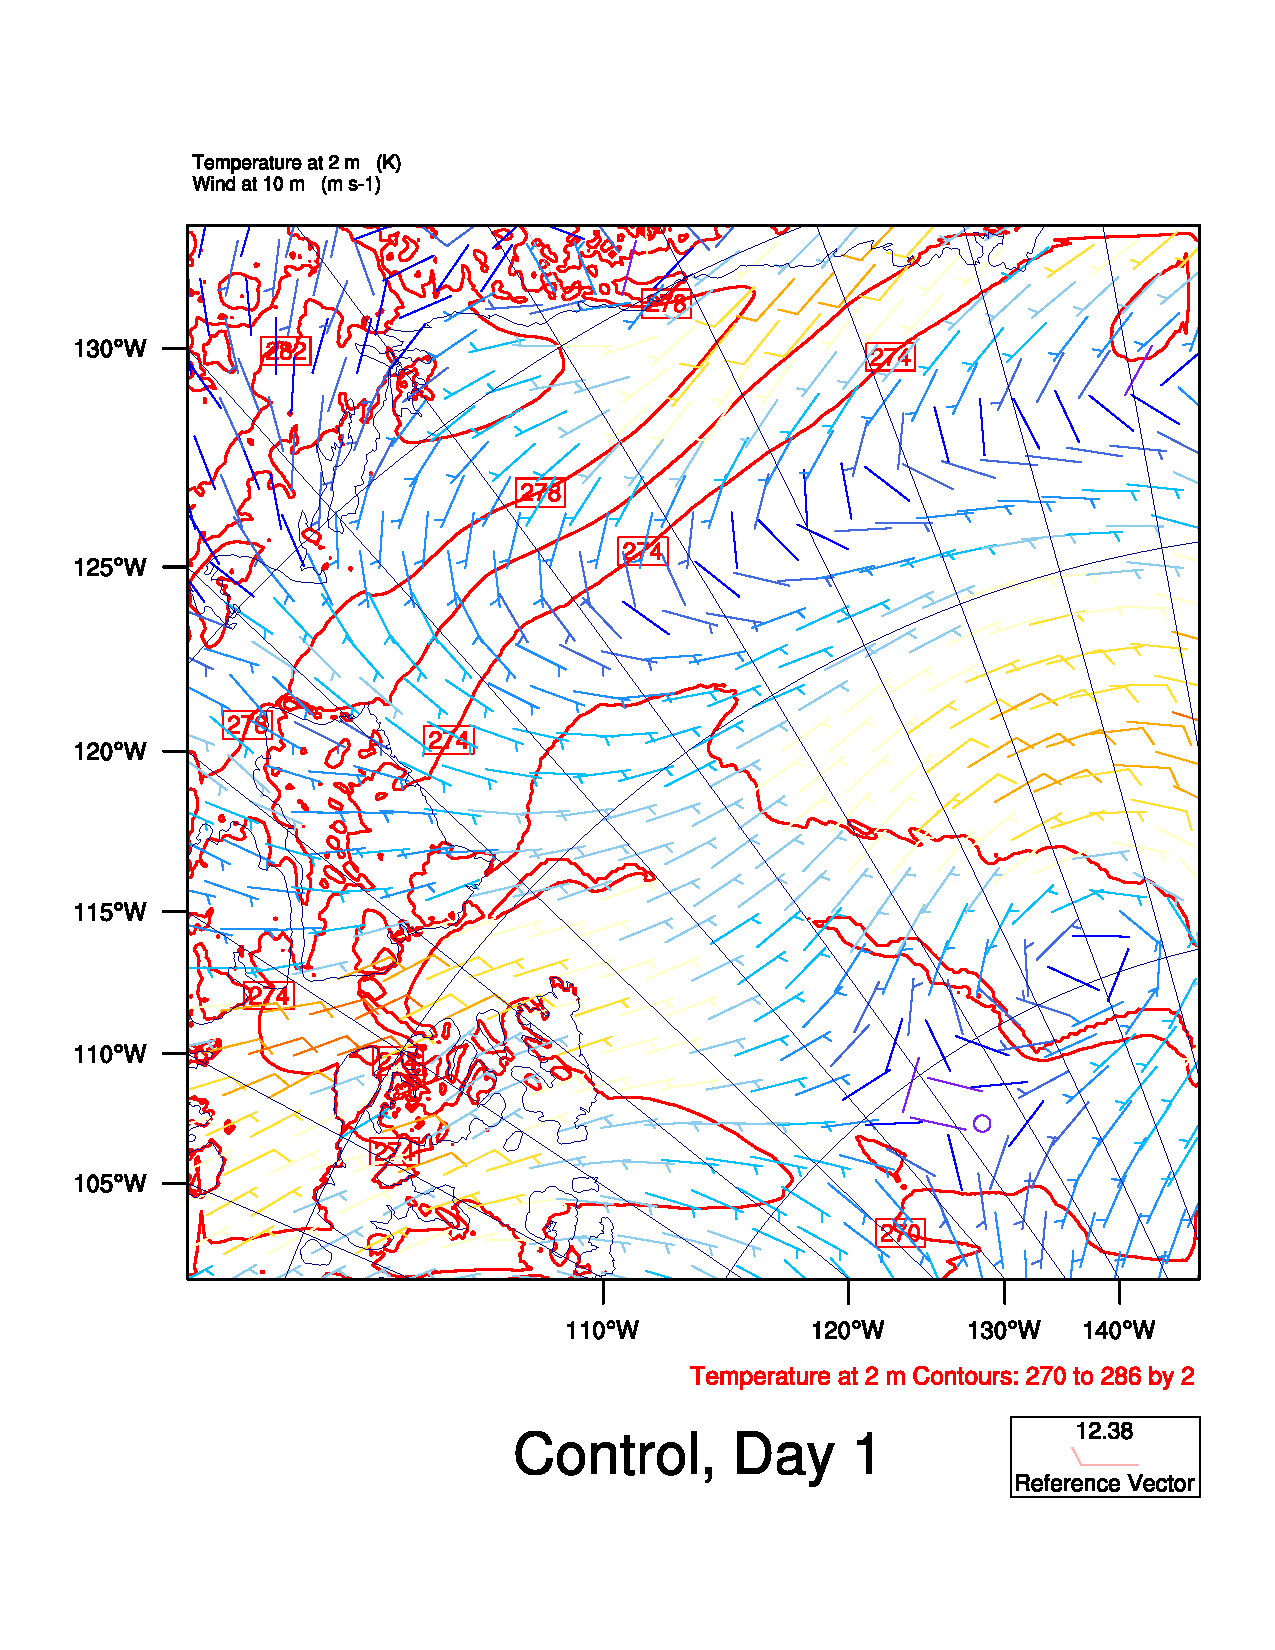
\includegraphics[width=\textwidth]{results/control/T2UV10_Control_Day1.pdf}
        \caption{Day 1}
        \label{subfig:weather_cont_day1}
    \end{subfigure}
    \begin{subfigure}{0.48\textwidth}
        \centering
        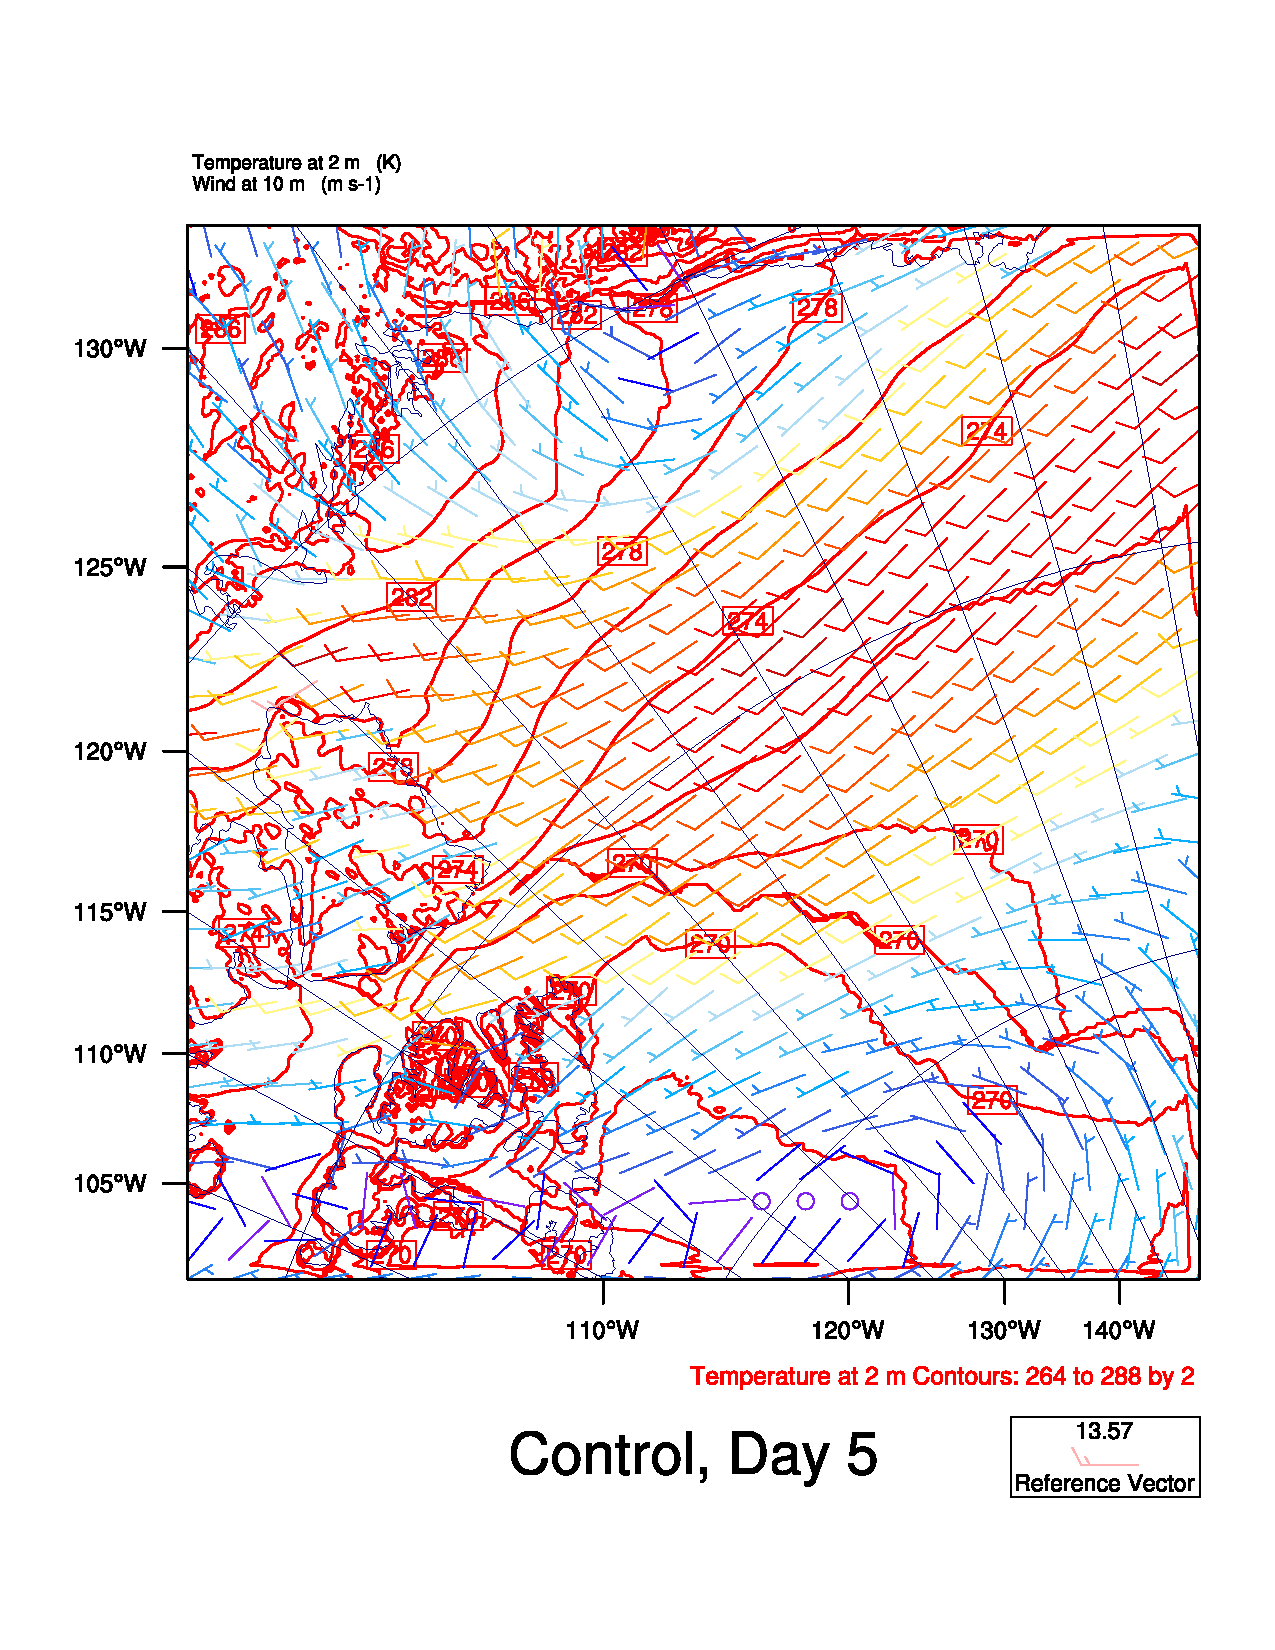
\includegraphics[width=\textwidth]{results/control/T2UV10_Control_Day5.pdf}
        \caption{Day 5}
        \label{subfig:weather_cont_day5}
    \end{subfigure}
    \caption{The temperature and wind pattern for days 1 and 5, from the control run. The temperature at 2~m height is represented by red contour lines and the wind speed and direction at 10~m height is shown by wind barbs and their color, where red indicates higher wind speed and blue indicates lower. The shortest tails on the wind barbs indicate a wind speed of 5~m/s and the longest indicate 10~m/s.}
    \label{fig:weather}
\end{figure}

By day 5 the wind direction has changed to south-easterly, see figure~\ref{subfig:weather_cont_day5}, and the clouds in the cross section, figure~\ref{subfig:cross_LWC_Day5} are low stratus over the sea ice, and there is also some thin cloud formation at the mountain, probably formed by weaker orographic lifting. There is no IWC in the section for day 5 (not shown). The stratus clouds in day 5 (figure~\ref{subfig:cross_LWC_Day5}) have highest LWC in the core of the clouds, where the temperature is lowest, there the temperature inversion stops the air from rising further. Following theory~\citep{Rogers1989}, LWC increases with height above cloud base and reaches its maximum at the cloud top. The LWC does rise with height above cloud base as expected, except for at the cloud top. Entrainment of dryer air at the top of clouds causes cloud droplets to evaporate and thereby thins the clouds~\citep{Wallace2006}.

\begin{figure}
    \centering
    \begin{subfigure}{0.48\textwidth}
        \centering
        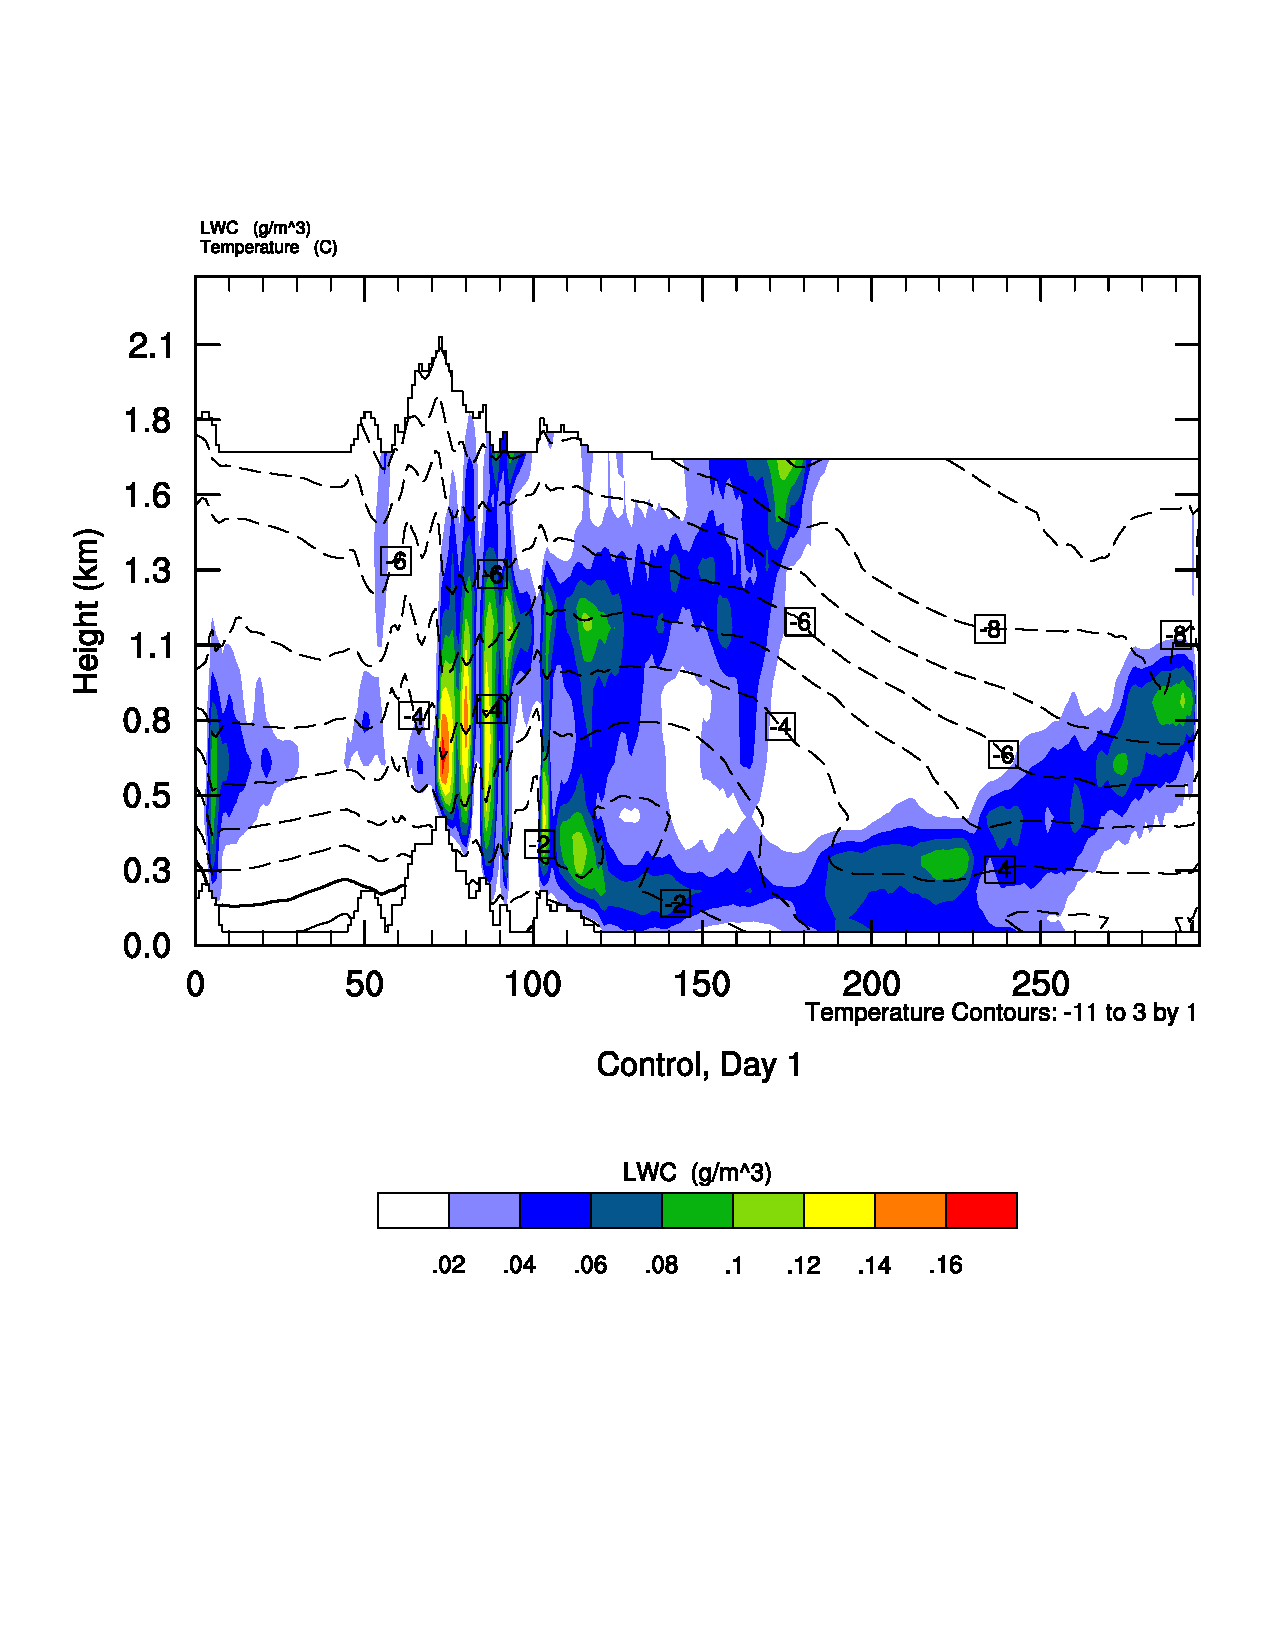
\includegraphics[width=\textwidth]{results/control/crossSec_LWC_Control_Day1.pdf}
        \caption{LWC and temperature, day 1.}
        \label{subfig:cross_LWC_day1}
    \end{subfigure}
    \begin{subfigure}{0.48\textwidth}
        \centering
        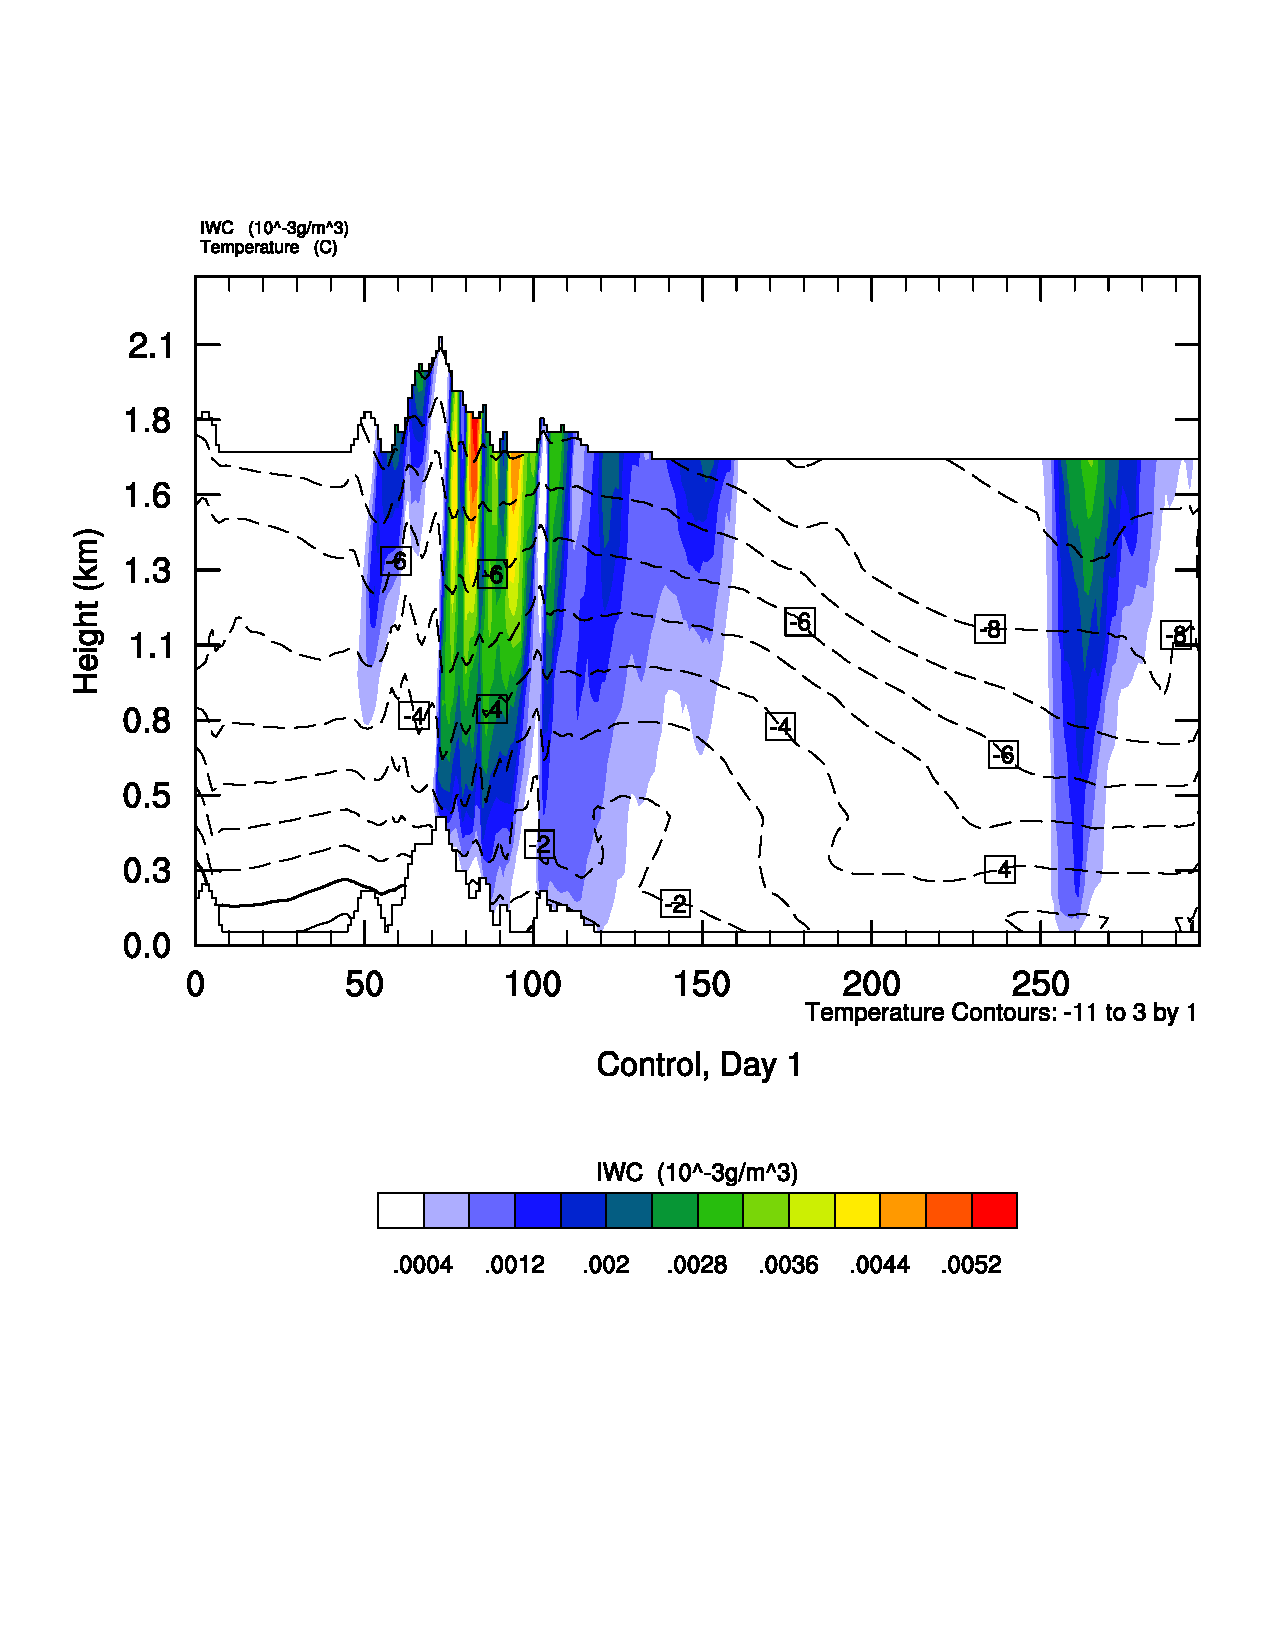
\includegraphics[width=\textwidth]{results/control/crossSec_IWC_Control_Day1.pdf}
        \caption{IWC and temperature, day1.}
        \label{subfig:cross_IWC_day1}
    \end{subfigure}
    
    \begin{subfigure}{0.48\textwidth}
        \centering
        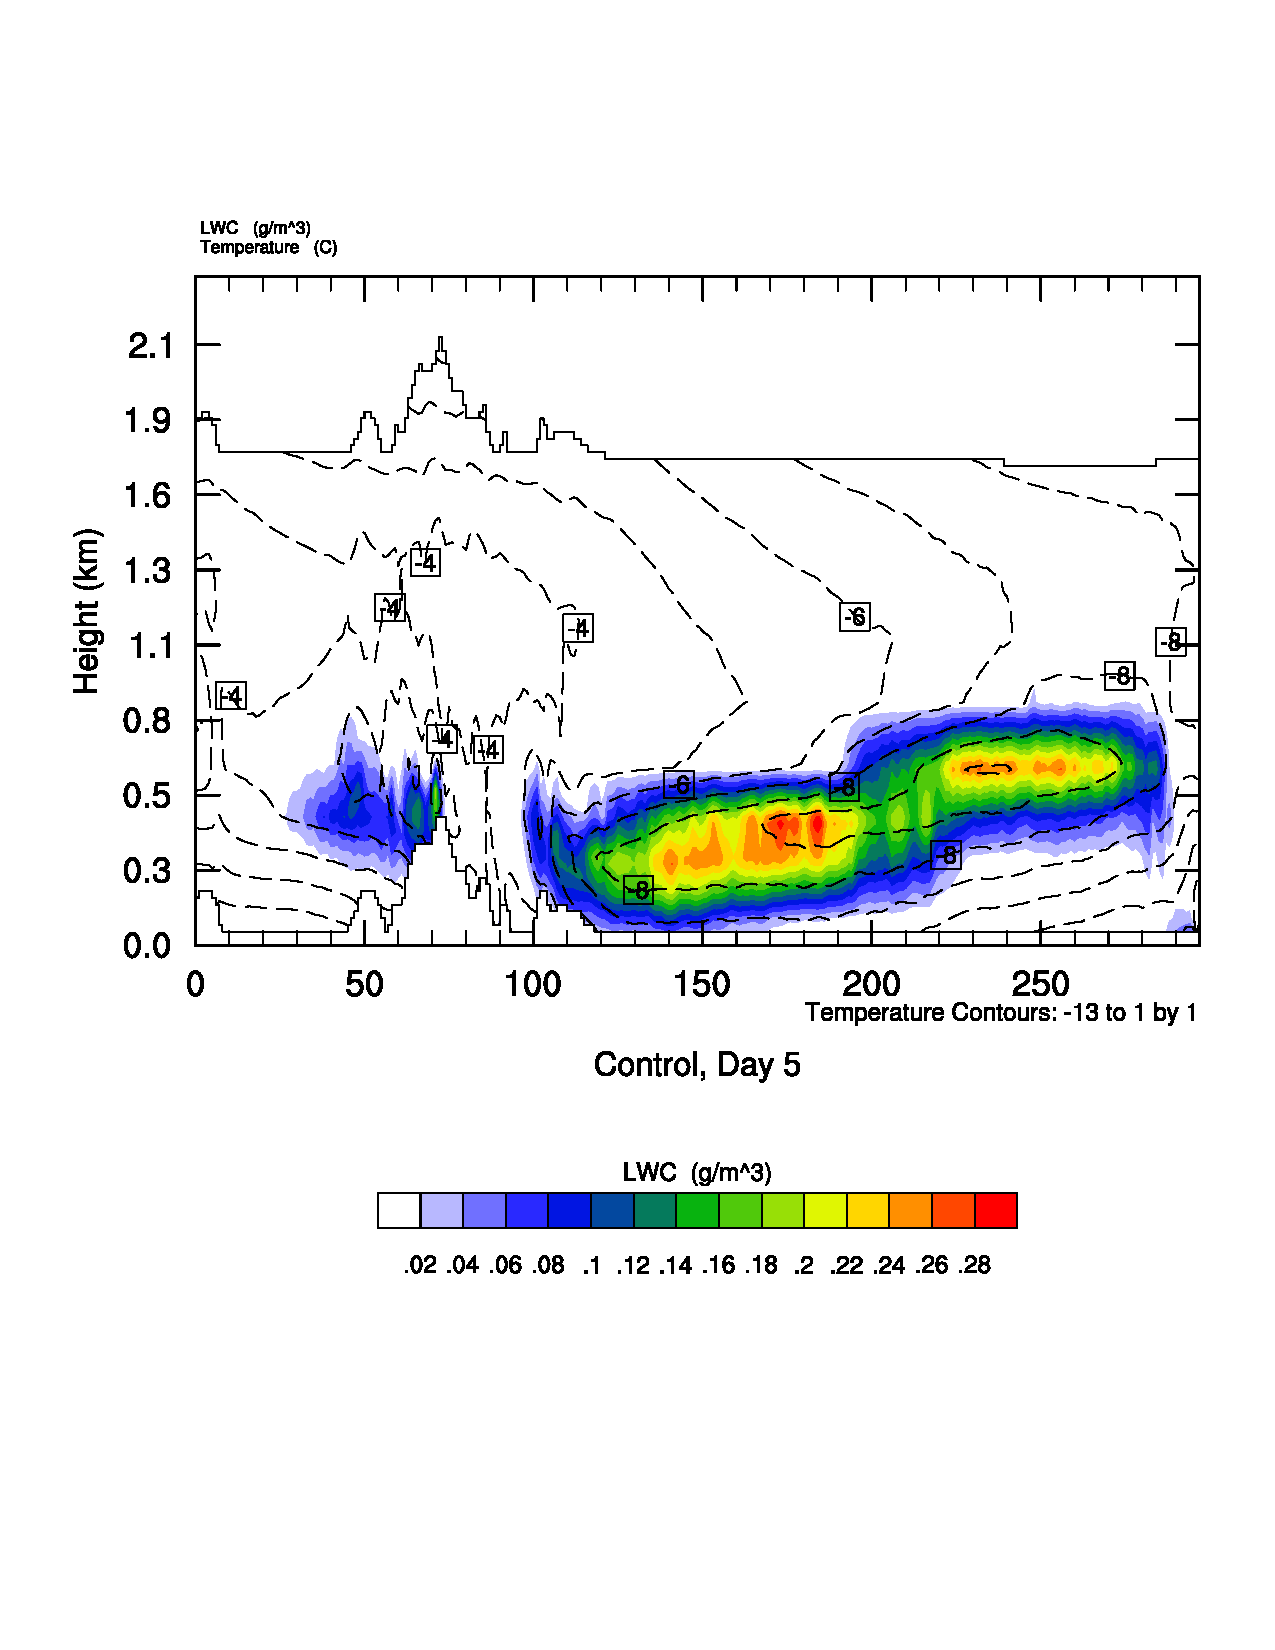
\includegraphics[width=\textwidth]{results/control/crossSec_LWC_Control_Day5.pdf}
        \caption{LWC and temperature, day 5.}
        \label{subfig:cross_LWC_Day5}
    \end{subfigure}
    \begin{subfigure}{0.48\textwidth}
        \centering
        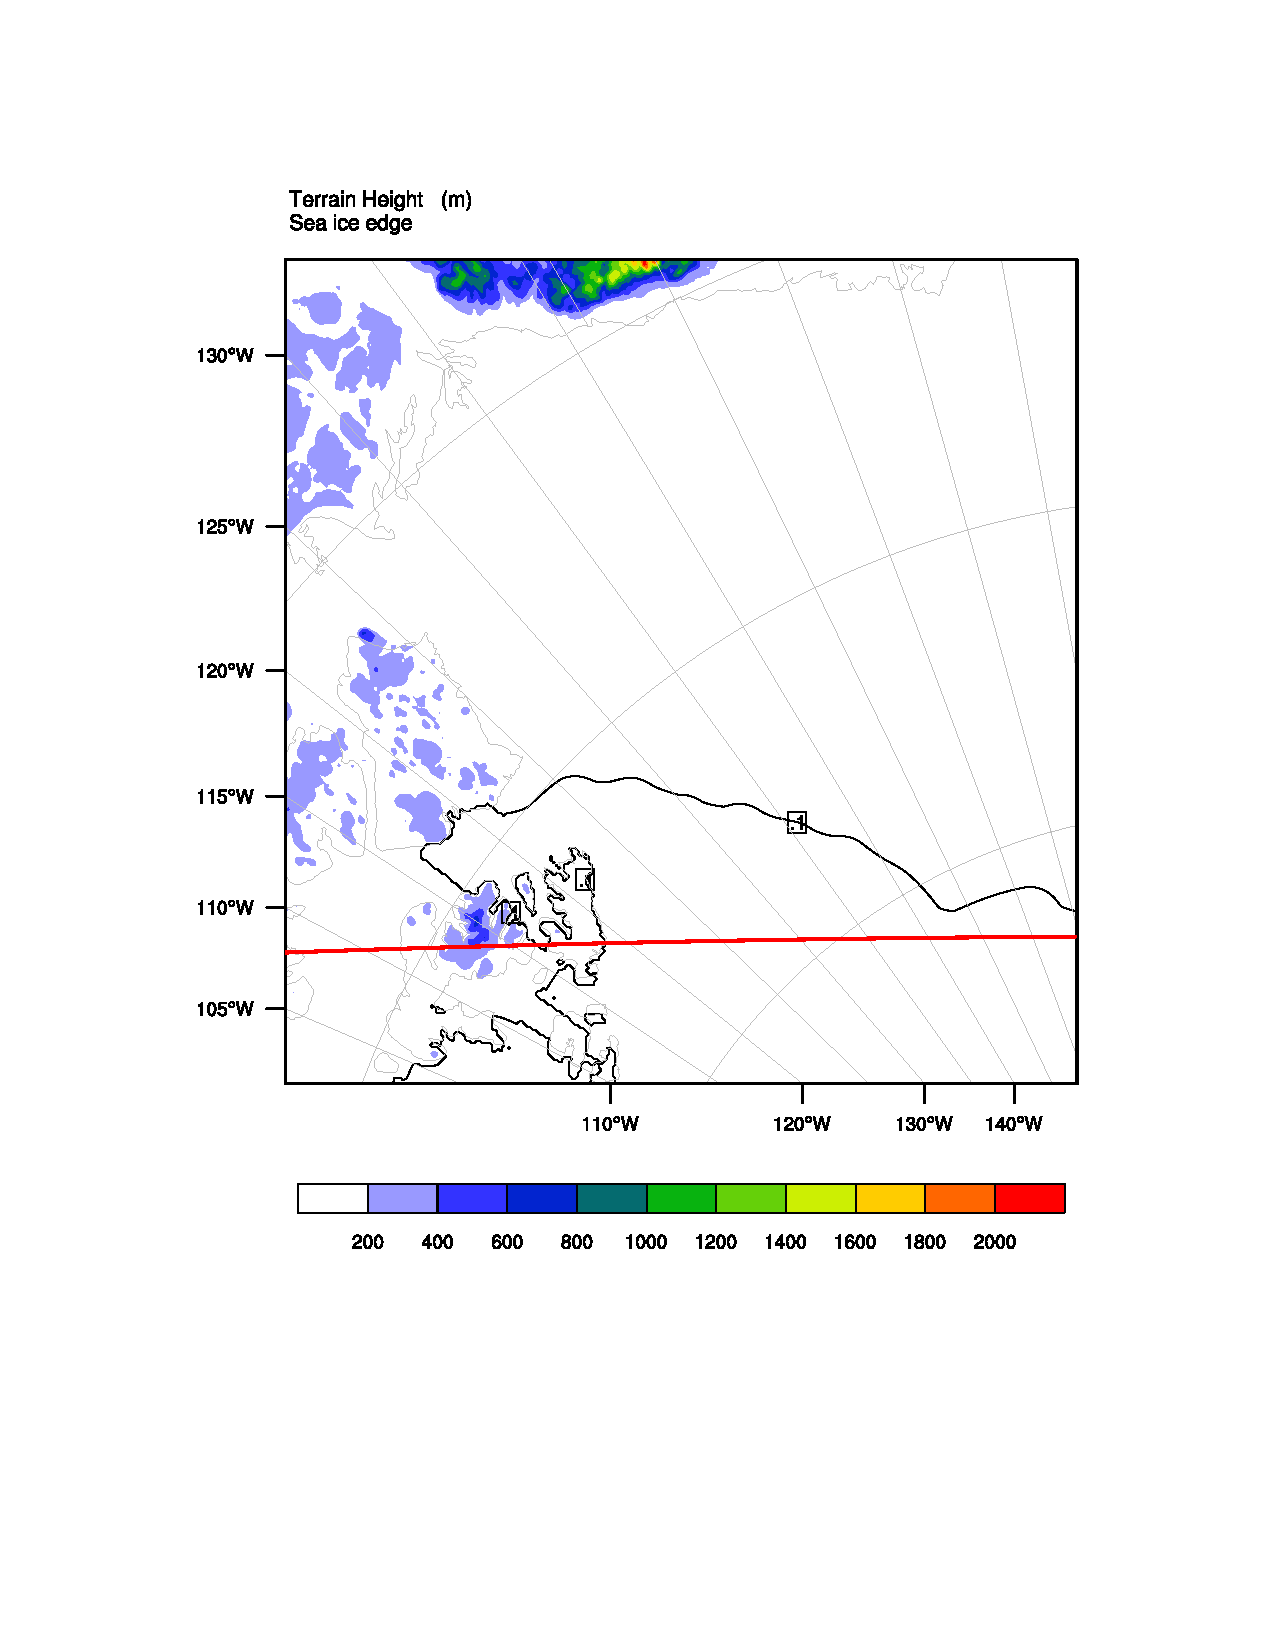
\includegraphics[width=\textwidth]{results/control/crossSec_line.pdf}
        \caption{Line over which the vertical cross sections are made.}
        \label{subfig:cross_line}
    \end{subfigure}
    \caption{Vertical cross sections of averaged liquid ($\text{g/m}^3$) and ice  ($\text{mg/m}^3$) water content, as filled contours, with temperature ($\degree\text{C}$) as dashed contours, from the control run, for days 1 and 5. LWC and IWC for day 1 are shown in figures~\ref{subfig:cross_LWC_day1} and~\ref{subfig:cross_IWC_day1} respectively. Figure~\ref{subfig:cross_LWC_Day5} shows the LWC for day 5. (Notice the different scales.) The IWC on day 5 was 0 in the section and is not shown. Figure~\ref{subfig:cross_line} shows a map of the area with the ice edge as a black contour line. Terrain height is represented by filled contours and the red line over the sea ice is the line over which the cross sections are made.}
    \label{fig:sections}
\end{figure}

The LWP, CDNC and $r_e$ for days 1 and 5 are shown in figure~\ref{fig:lwpcdncre_r1}. One can see that the LWP and the CDNC have similar pattern, which is expected based on equation~\ref{eqn:LWC}. The pattern in $r_e$ also fits quite well with that of LWP, where the effective droplet radius is higher so is LWP, which can be interpreted as that larger droplets contain more water. These similarities in patterns are true for both days 1 and 5. In the daily averaged LWP for day 1, figure~\ref{subfig:LWPr1Day1}, there are some areas with LWP of 0-20~$\text{g/m}^2$, for instance 78-81$\degree$N 135-145$\degree$W. Here there are no low clouds, which is also evident from the lack of number of droplets per cubic centimeter in figure~\ref{subfig:cdnc_cont_Day1}. This figure shows the numbers with units $10^6~\text{kg}^{-1}$, which can be approximated to the more common units for CDNC, per cubic centimeter ($\text{cm}^{-3}$). Assuming that the clouds are close enough to the surface to assume an air density $\rho_a = 1~\text{kg/m}^3=1~\text{kg/}10^6\text{cm}^3$, then for CDNC $10^6/\text{kg} = \text{cm}^{-3}$ is a good approximation.
Based on the LWP from day 5 (figure~\ref{subfig:LWPr1Day5}), most of the low clouds were only in the western part of the domain on that day. Particularly thick low clouds are seen just south of 75$\degree$N and west of 130$\degree$W. Where the LWP ranges from 100 to almost 300~$\text{g/m}^2$, and the CDNC ranges from 15 to 60~$\text{cm}^{-3}$ (figure~\ref{subfig:cdnc_cont_Day5}). These clouds contain many droplets with averaged effective radius as large as 8~$\mu\text{m}$ (figure~\ref{subfig:recloud_r1Day5}).

%---------- LWP control run, days 1 and 5
\begin{figure}
    \centering
    \begin{subfigure}{0.40\textwidth}
        \centering
        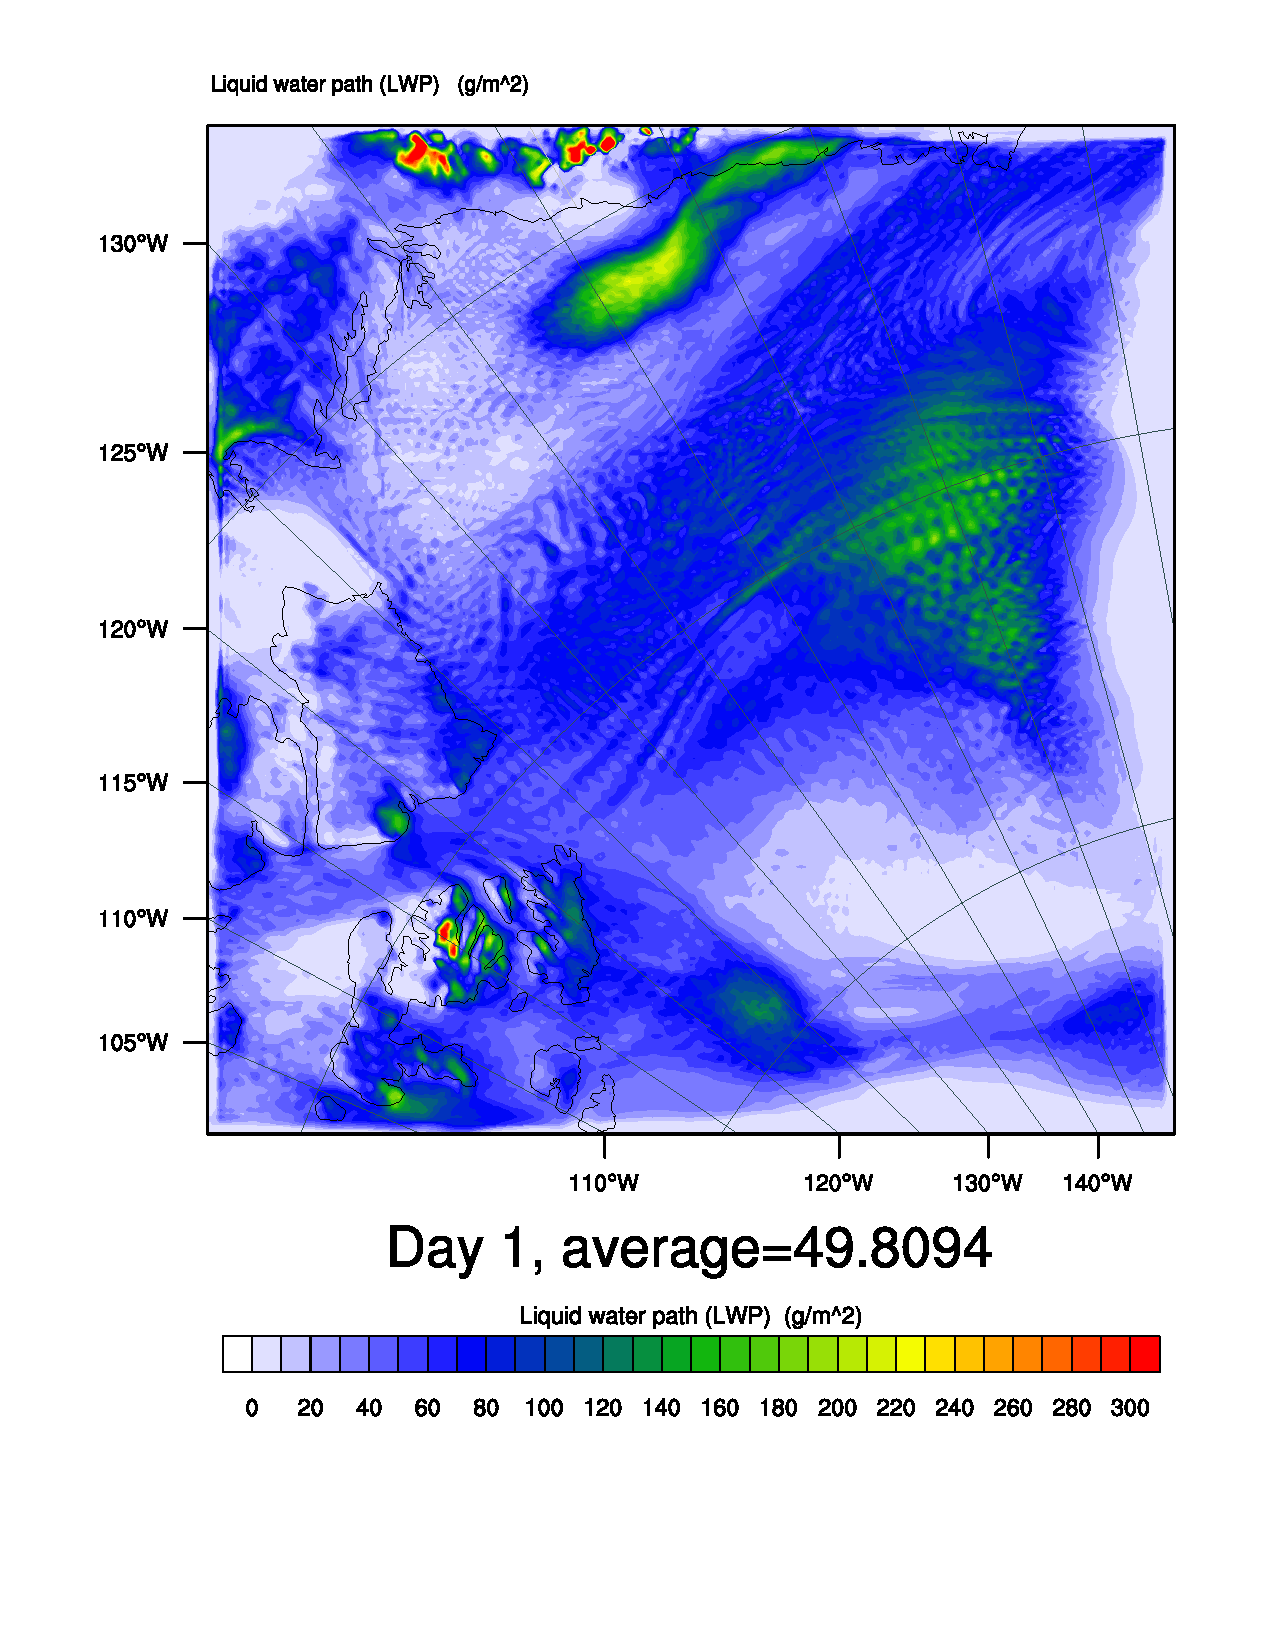
\includegraphics[width=\textwidth]{results/control/LWP_Day1.pdf}
        \caption{LWP day 1.}
        \label{subfig:LWPr1Day1}
    \end{subfigure}
    \begin{subfigure}{0.40\textwidth}
        \centering
        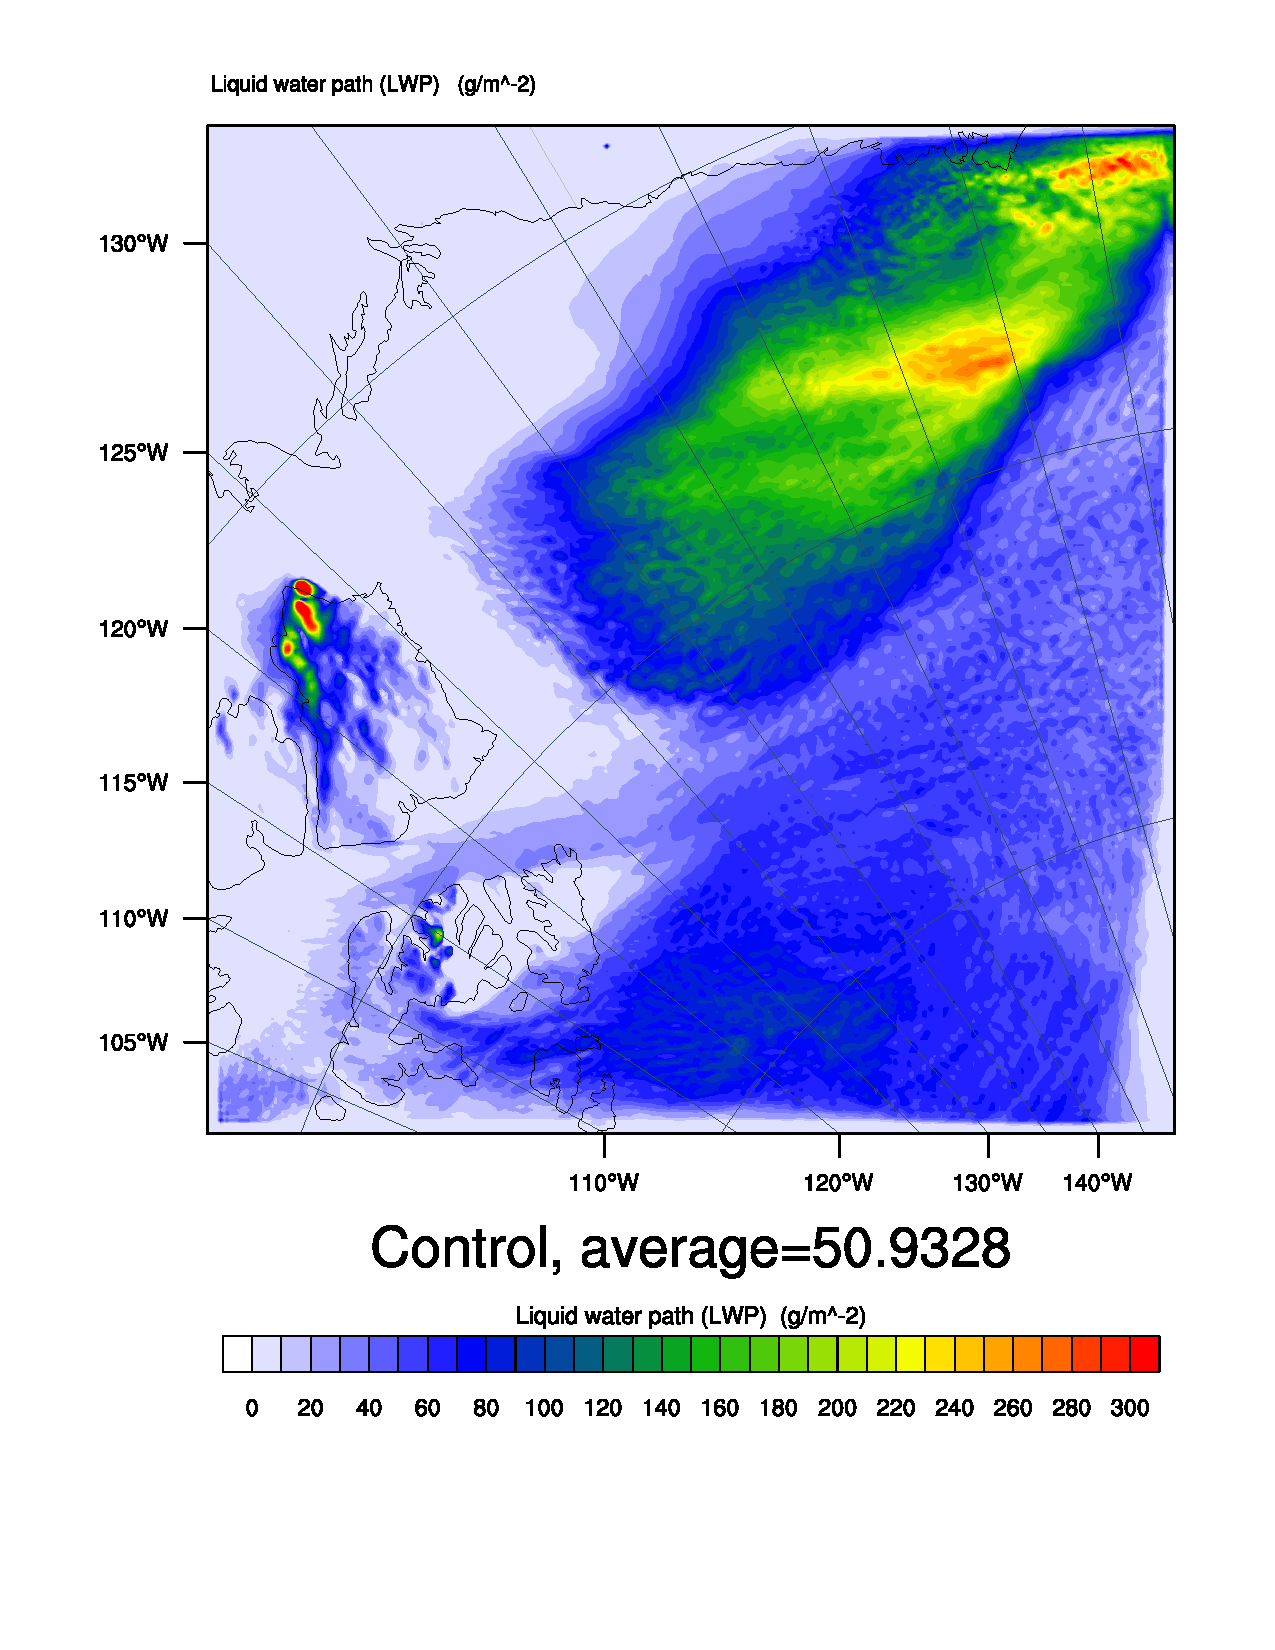
\includegraphics[width=\textwidth]{results/control/LWP_Day5.pdf}
        \caption{LWP day 5.}
        \label{subfig:LWPr1Day5}
    \end{subfigure}

%------CDNC
	\begin{subfigure}{0.40\textwidth}
		\centering
		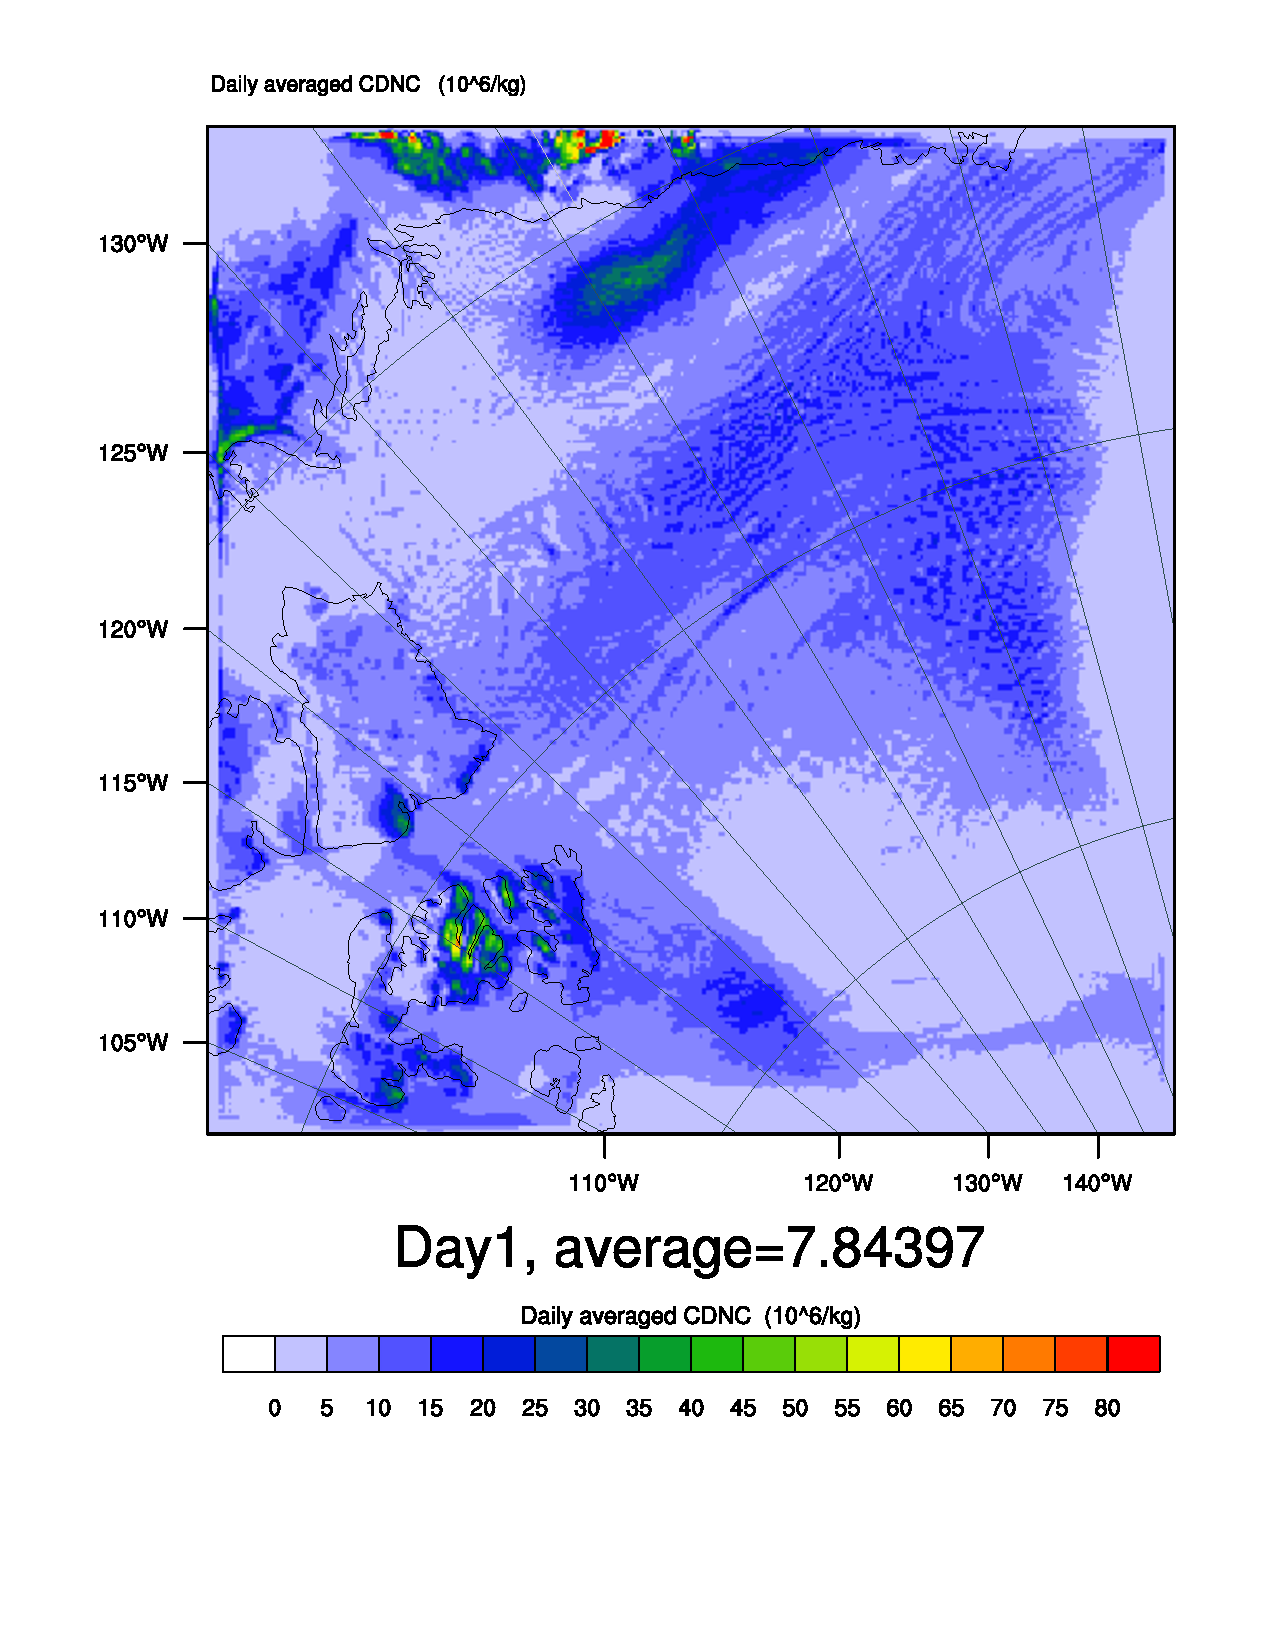
\includegraphics[width=\textwidth]{results/control/QNCLOUD_Day1.pdf}
		\caption{CDNC day 1.}
		\label{subfig:cdnc_cont_Day1}
	\end{subfigure}
	\begin{subfigure}{0.40\textwidth}
		\centering
		\includegraphics[width=\textwidth]{results/control/QNCLOUD_day5.pdf}
		\caption{CDNC day 5.}
		\label{subfig:cdnc_cont_Day5}
	\end{subfigure}
	
%----------- Effective radius, days 1 and 5
	\begin{subfigure}{0.40\textwidth}
		\centering
		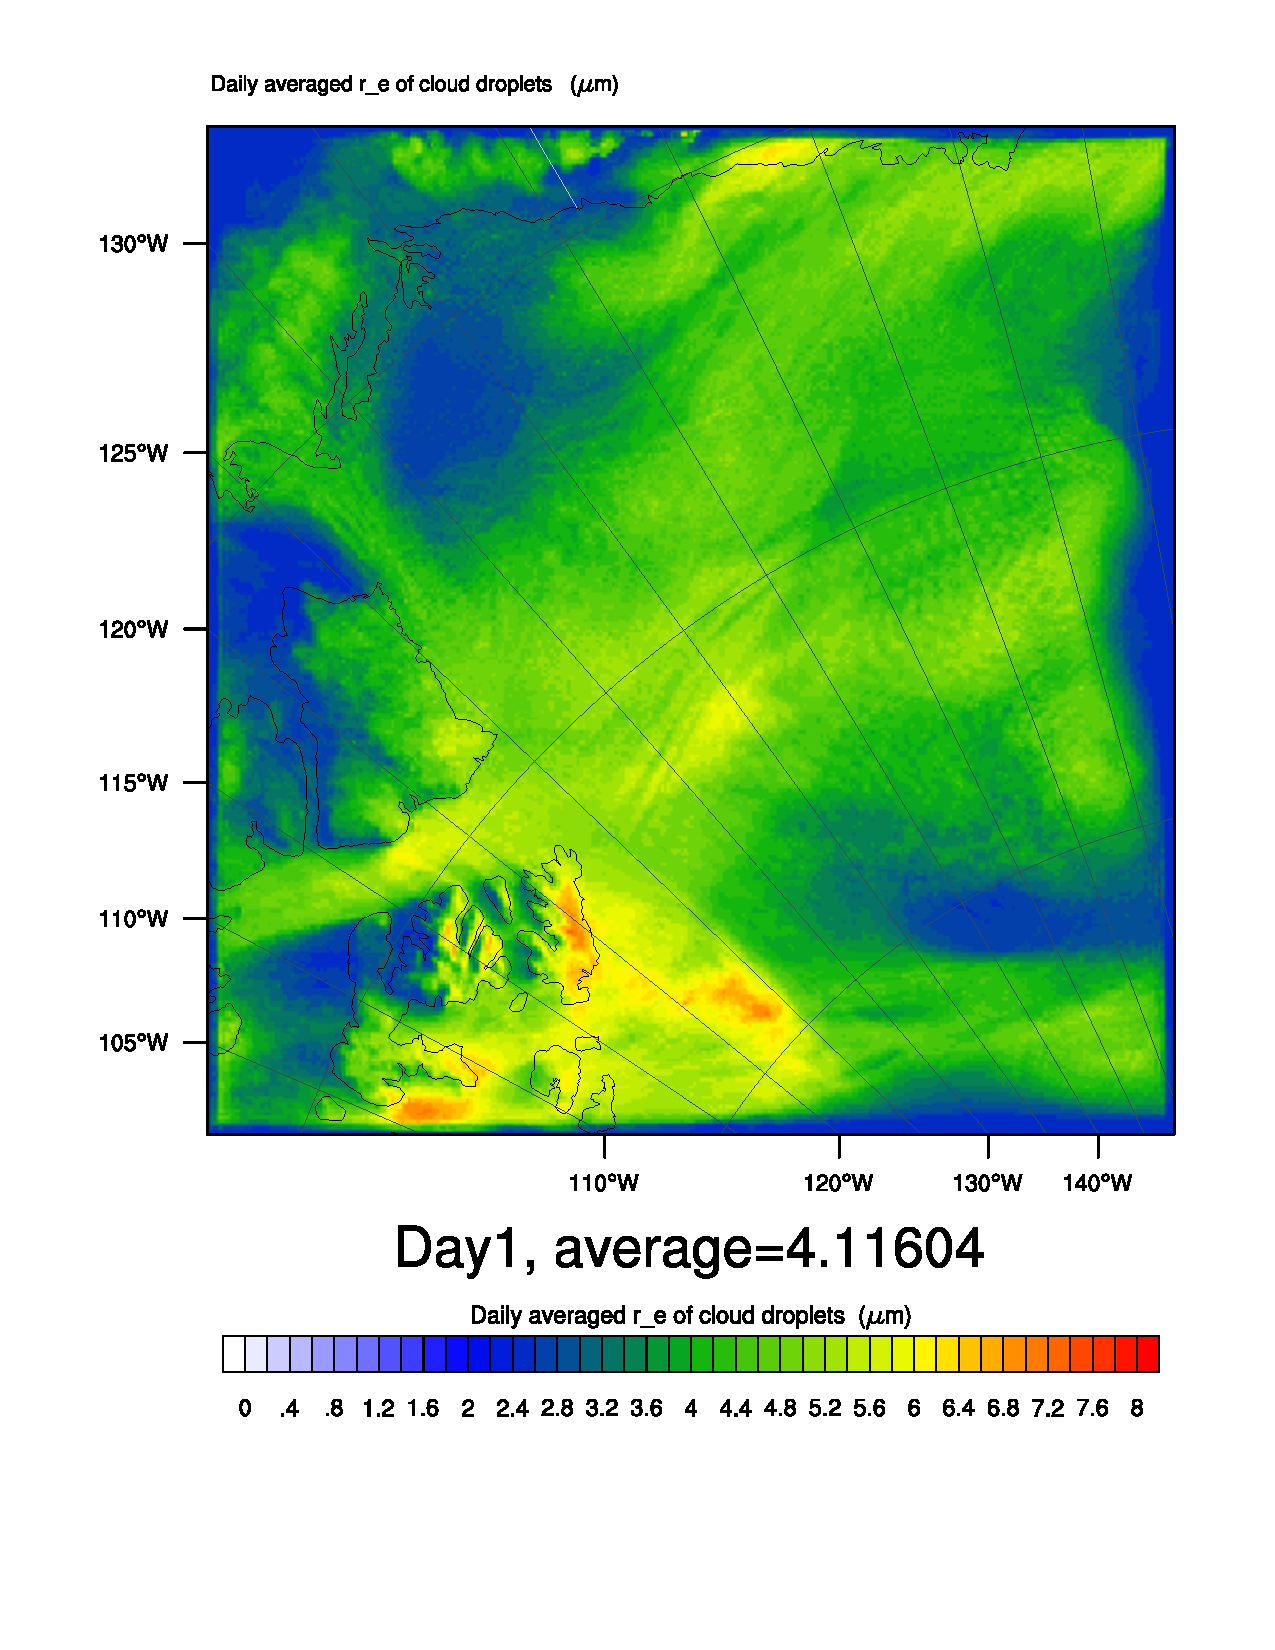
\includegraphics[width=\textwidth]{results/control/RE_CLOUD_Day1.pdf}
		\caption{$r_e$ day1.}
		\label{subfig:recloud_r1Day1}
	\end{subfigure}
	\begin{subfigure}{0.40\textwidth}
		\centering
		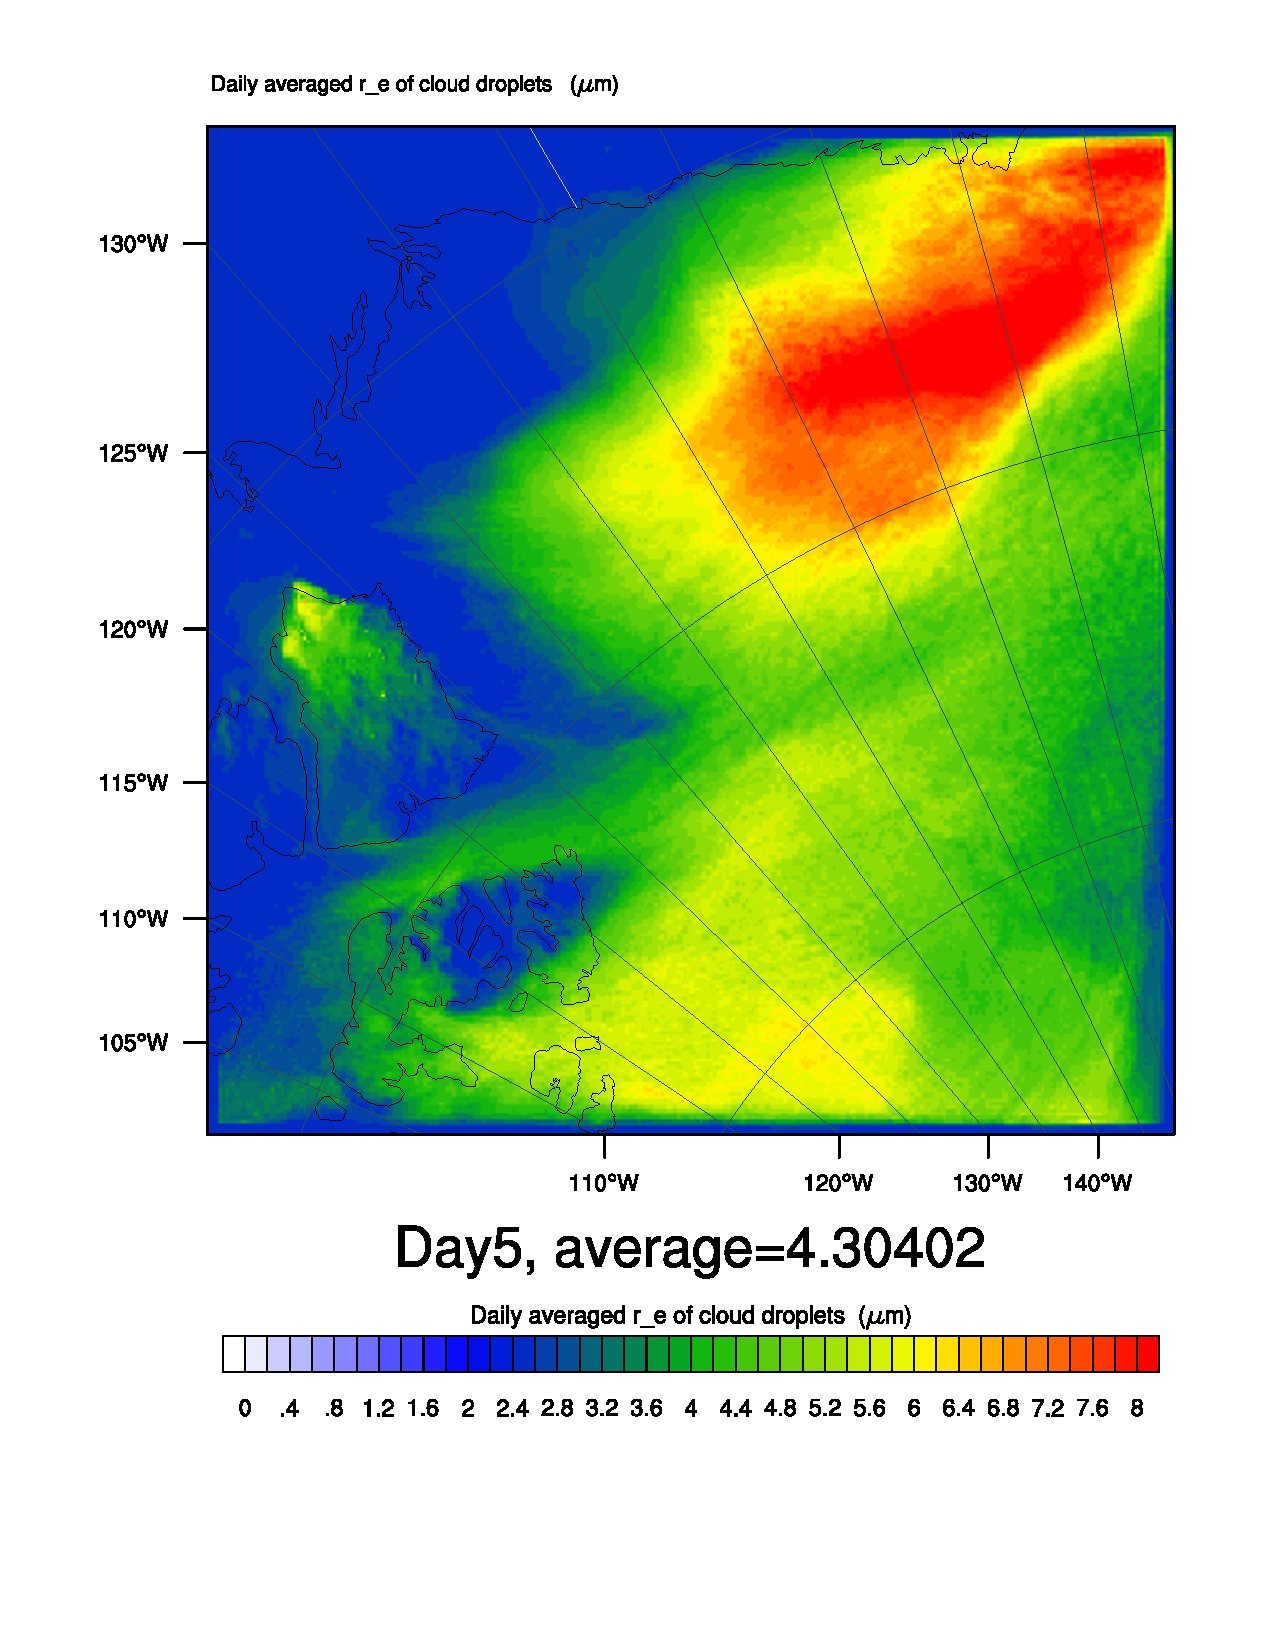
\includegraphics[width=\textwidth]{results/control/RE_CLOUD_Day5.pdf}
		\caption{$r_e$ day 5.}
		\label{subfig:recloud_r1Day5}
	\end{subfigure}
	\caption{LWP averaged in time, and CDNC and $r_e$ averaged over the lowermost 11 layers and time, for days 1 and 5. Control.}
	\label{fig:lwpcdncre_r1}
\end{figure}

Figure~\ref{subfig:swdown_r1Day1} shows the time averaged downwelling SW radiation at the surface. There the dark blue colors, indicating less downwelling shortwave radiation, fit well with the pattern for LWP in figure~\ref{subfig:LWPr1Day1}. Meaning that there are low clouds in the study area that that don't let much SW through, in fact most of it is reflected. The SW up at the top of the atmosphere (TOA) (figure~\ref{subfig:swup_r1Day1}) has the inverse pattern of SW down at the surface (figure~\ref{subfig:swdown_r1Day1}), which both fit well with the pattern in LWP for the low clouds, thus indicating that the low clouds have reflected much of the SW up at TOA. The effect of the low clouds can also be seen in the figures for LW radiation, where all the green in figure~\ref{subfig:glw_r1Day1} indicates a LW radiation flux downward at the surface of 270-200~$\text{W/m}^2$. This pattern of green is also recognized as a good fit with the LWP of the lower 1800~m of the atmosphere on day 1 (figure~\ref{subfig:LWPr1Day1}). The LW up at TOA (figure~\ref{subfig:lwup_r1Day1} on the other hand does not show the same values as for the downward LW. The LW up at TOA lies mostly in the range 195-225~$\text{W/m}^2$. The average value for the field is $215.5~\text{W/m}^2$, which is almost 60~$\text{W/m}^2$ less than the average 272.6~$\text{W/m}^2$ downward at the surface. Therefore there must be clouds higher up absorbing and re-emitting the LW radiation at lower temperatures, which according to Stefan-Boltzmann's law (equation~\ref{eqn:stefanboltzmann}) yields a smaller flux.

It is interesting to notice from figure~\ref{fig:radiation_r1Day1} that the downwelling LW at the surface, on average 272.6~$\text{W/m}^2$ (figure~\ref{subfig:glw_r1Day1}), is about three and a half times the average upwelling SW at TOA, of 76.9~$\text{W/m}^2$ (figure~\ref{subfig:swup_r1Day1}). Hence, in this case the low clouds had a warming effect at the surface 1st of September 2012.

%----------Radiation Day 1
\begin{figure}
\centering
	\begin{subfigure}{0.48\textwidth}
		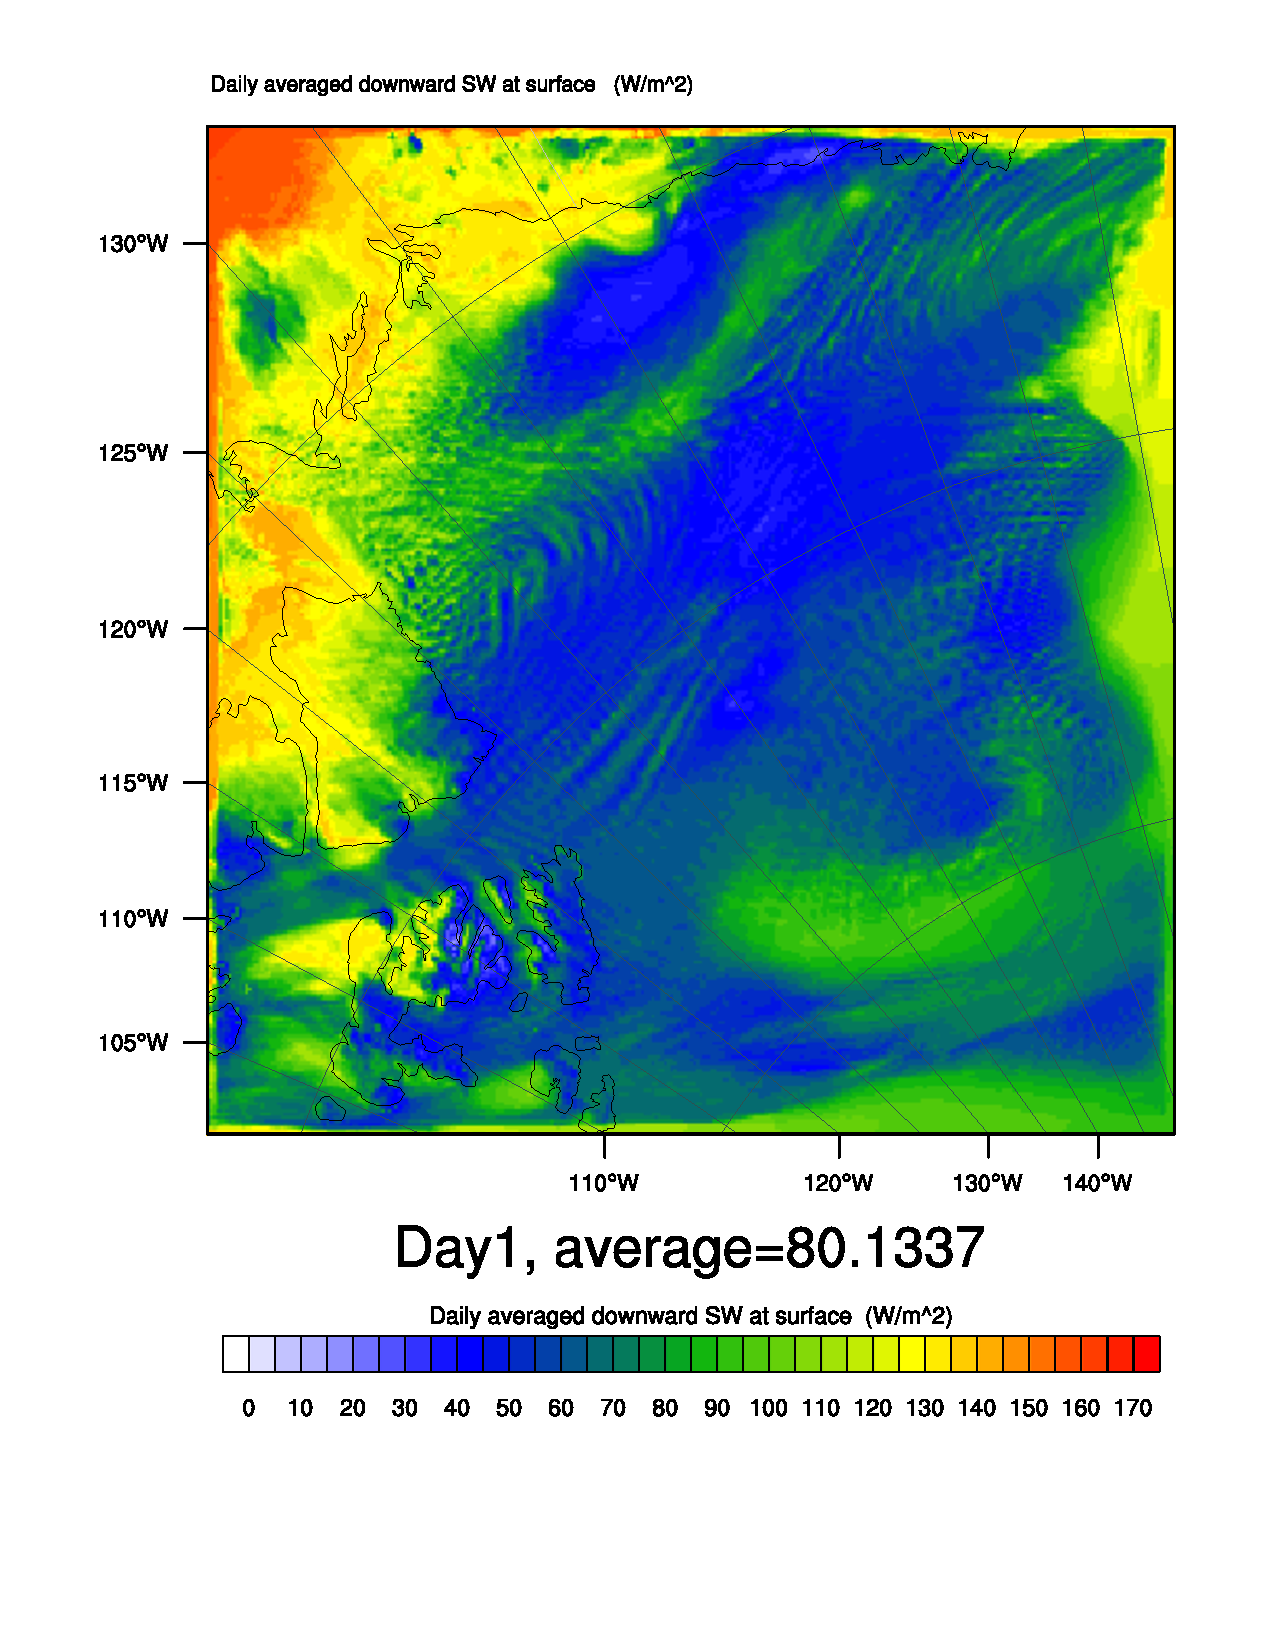
\includegraphics[width=\textwidth]{results/control/SWDOWN_Day1.pdf}
		\caption{SW down at the surface, day 1.}
		\label{subfig:swdown_r1Day1}
	\end{subfigure}
	\quad
	\begin{subfigure}{0.48\textwidth}
		\centering
		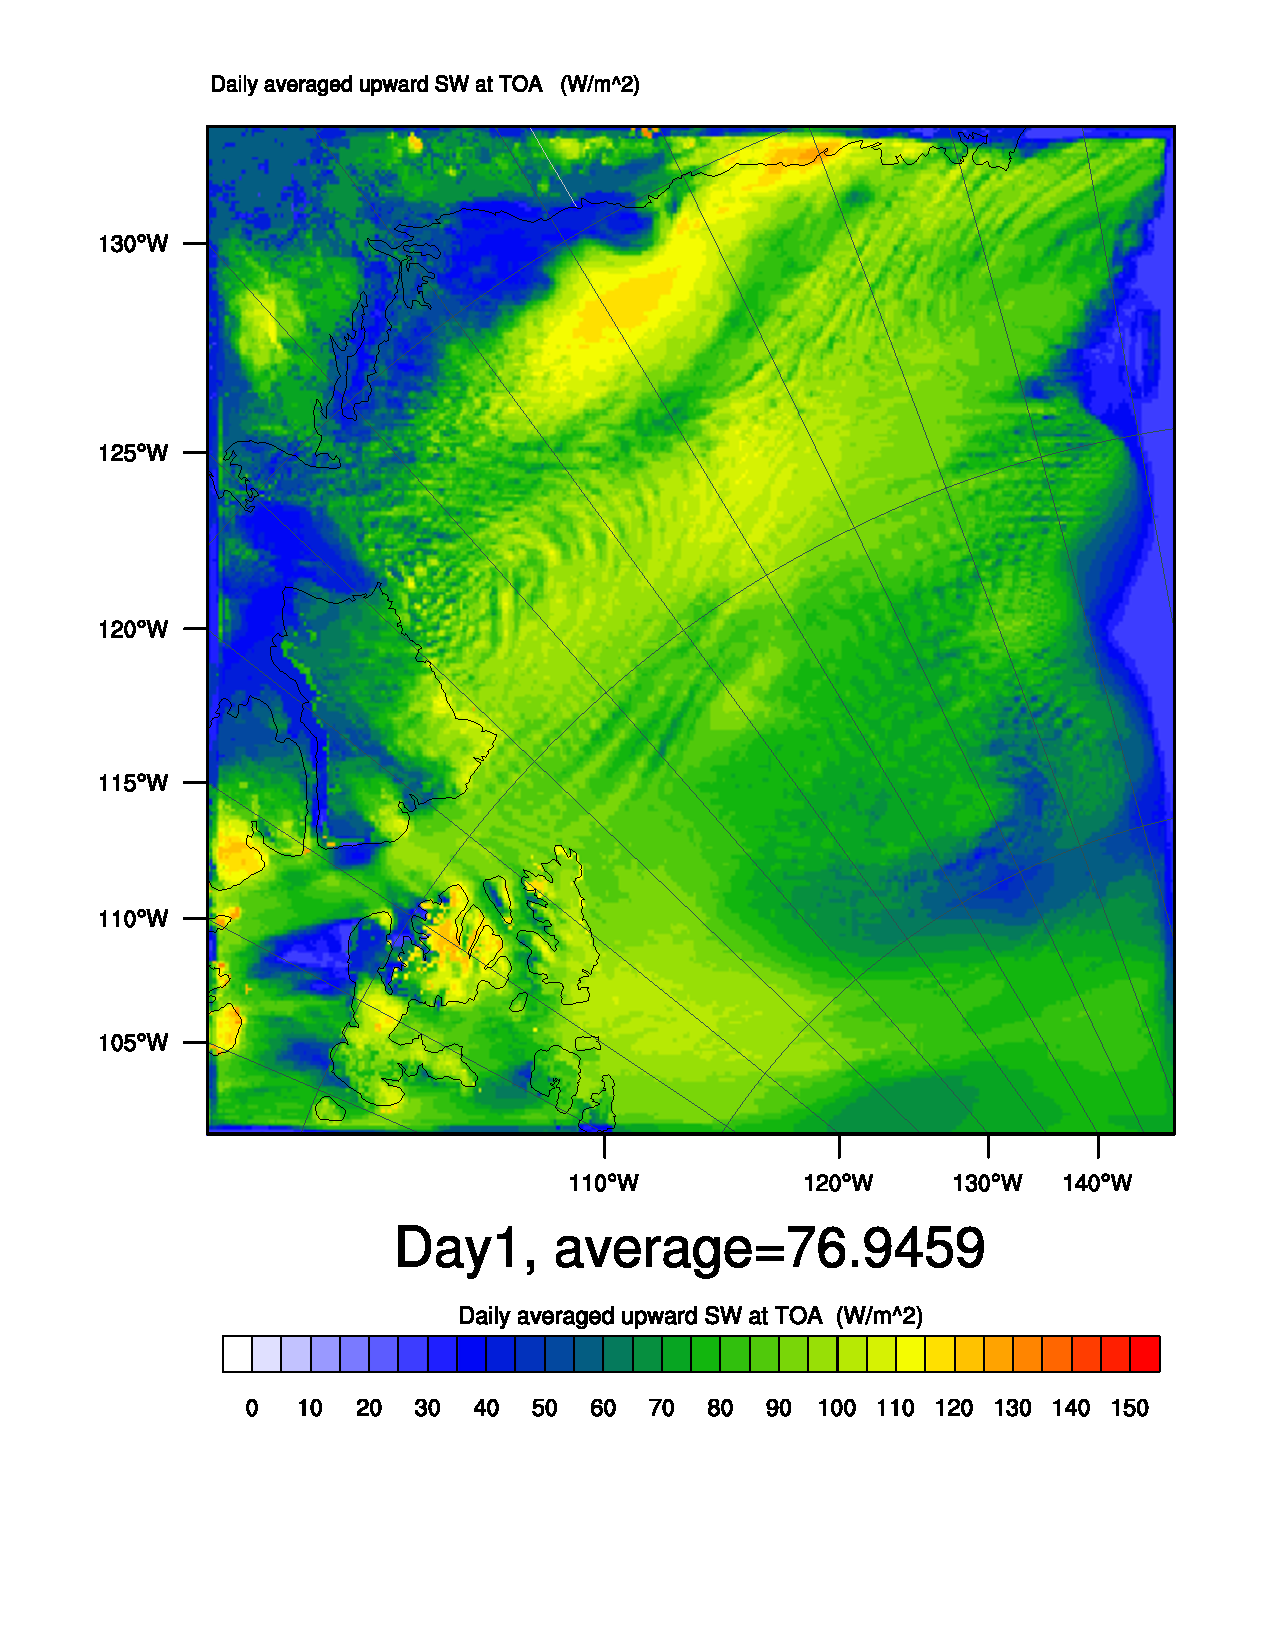
\includegraphics[width=\textwidth]{results/control/SWUPT_Day1.pdf}
		\caption{SW up at TOA, day 1.}
		\label{subfig:swup_r1Day1}
	\end{subfigure}
	
	\begin{subfigure}{0.48\textwidth}
		\centering
		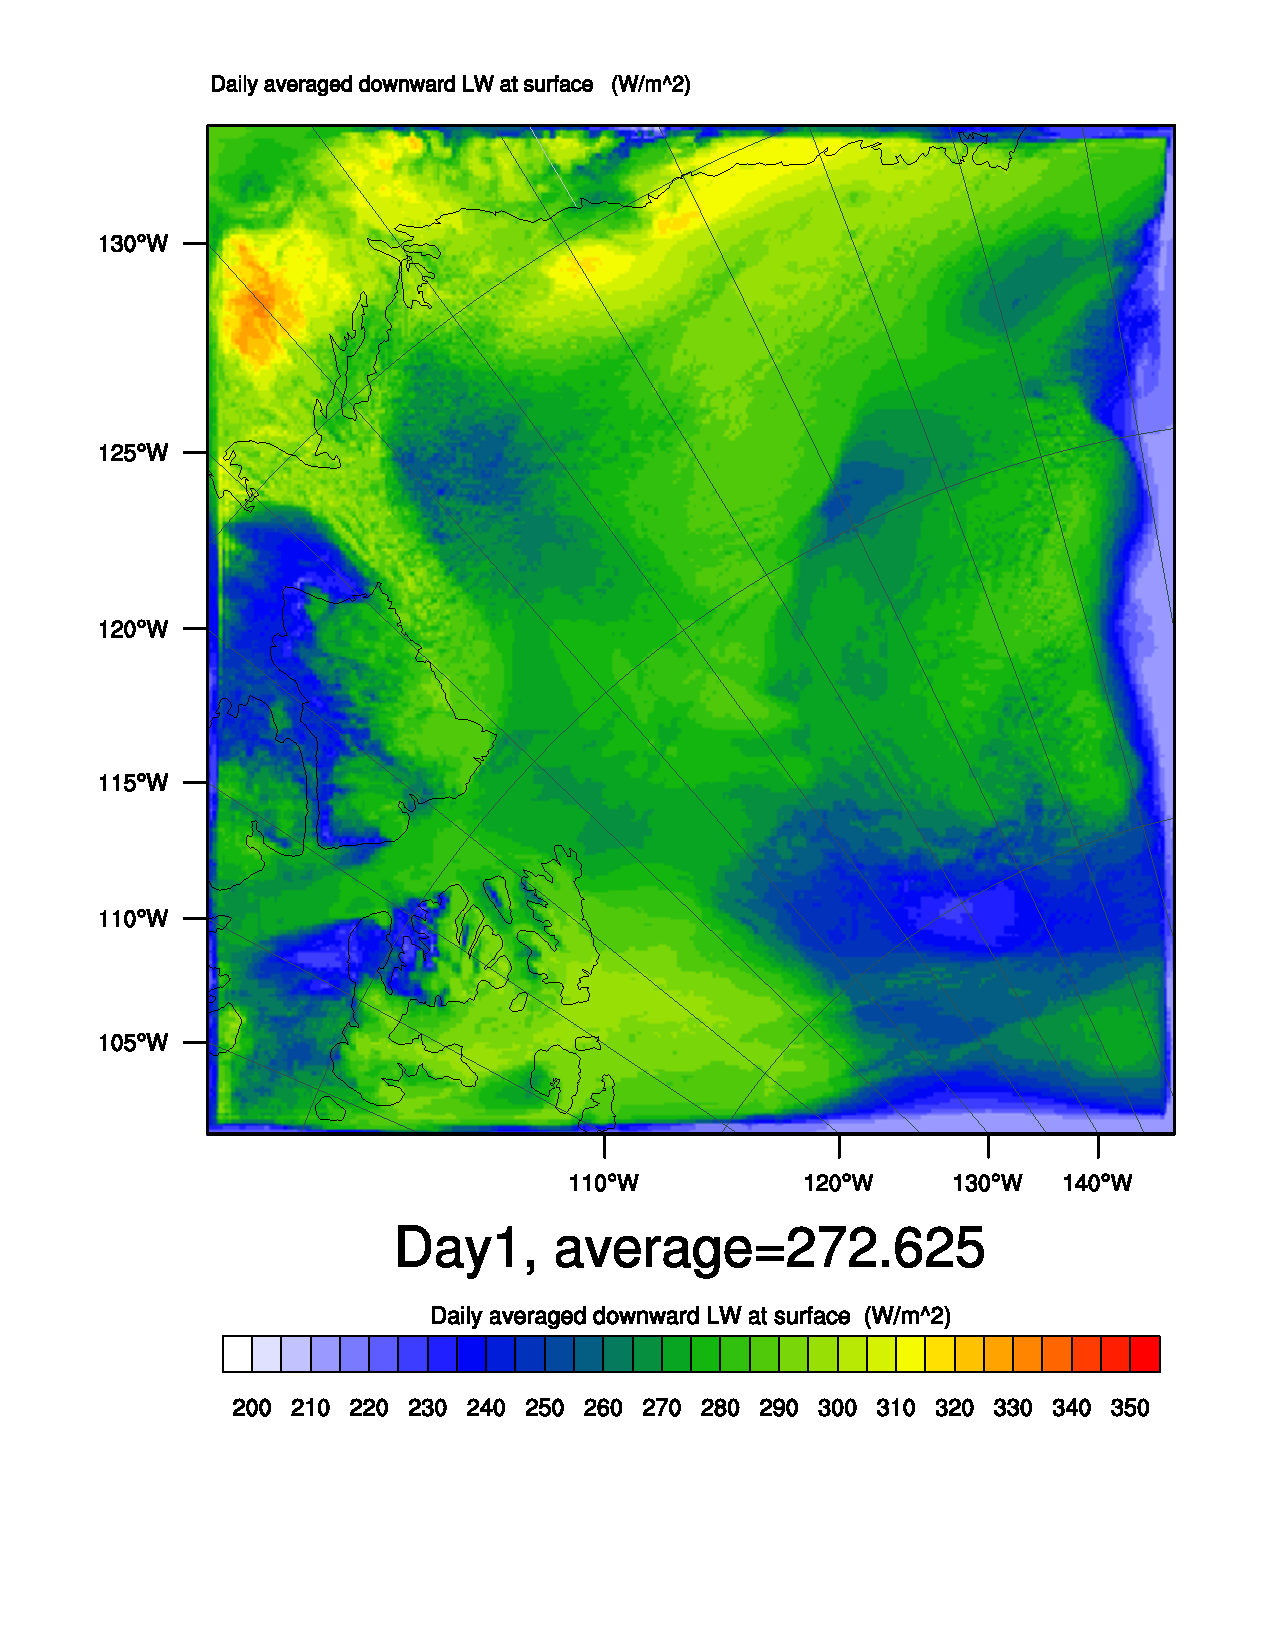
\includegraphics[width=\textwidth]{results/control/GLW_Day1.pdf}
		\caption{LW down at the surface, day 1.}
		\label{subfig:glw_r1Day1}
	\end{subfigure}
	\quad
	\begin{subfigure}{0.48\textwidth}
		\centering
		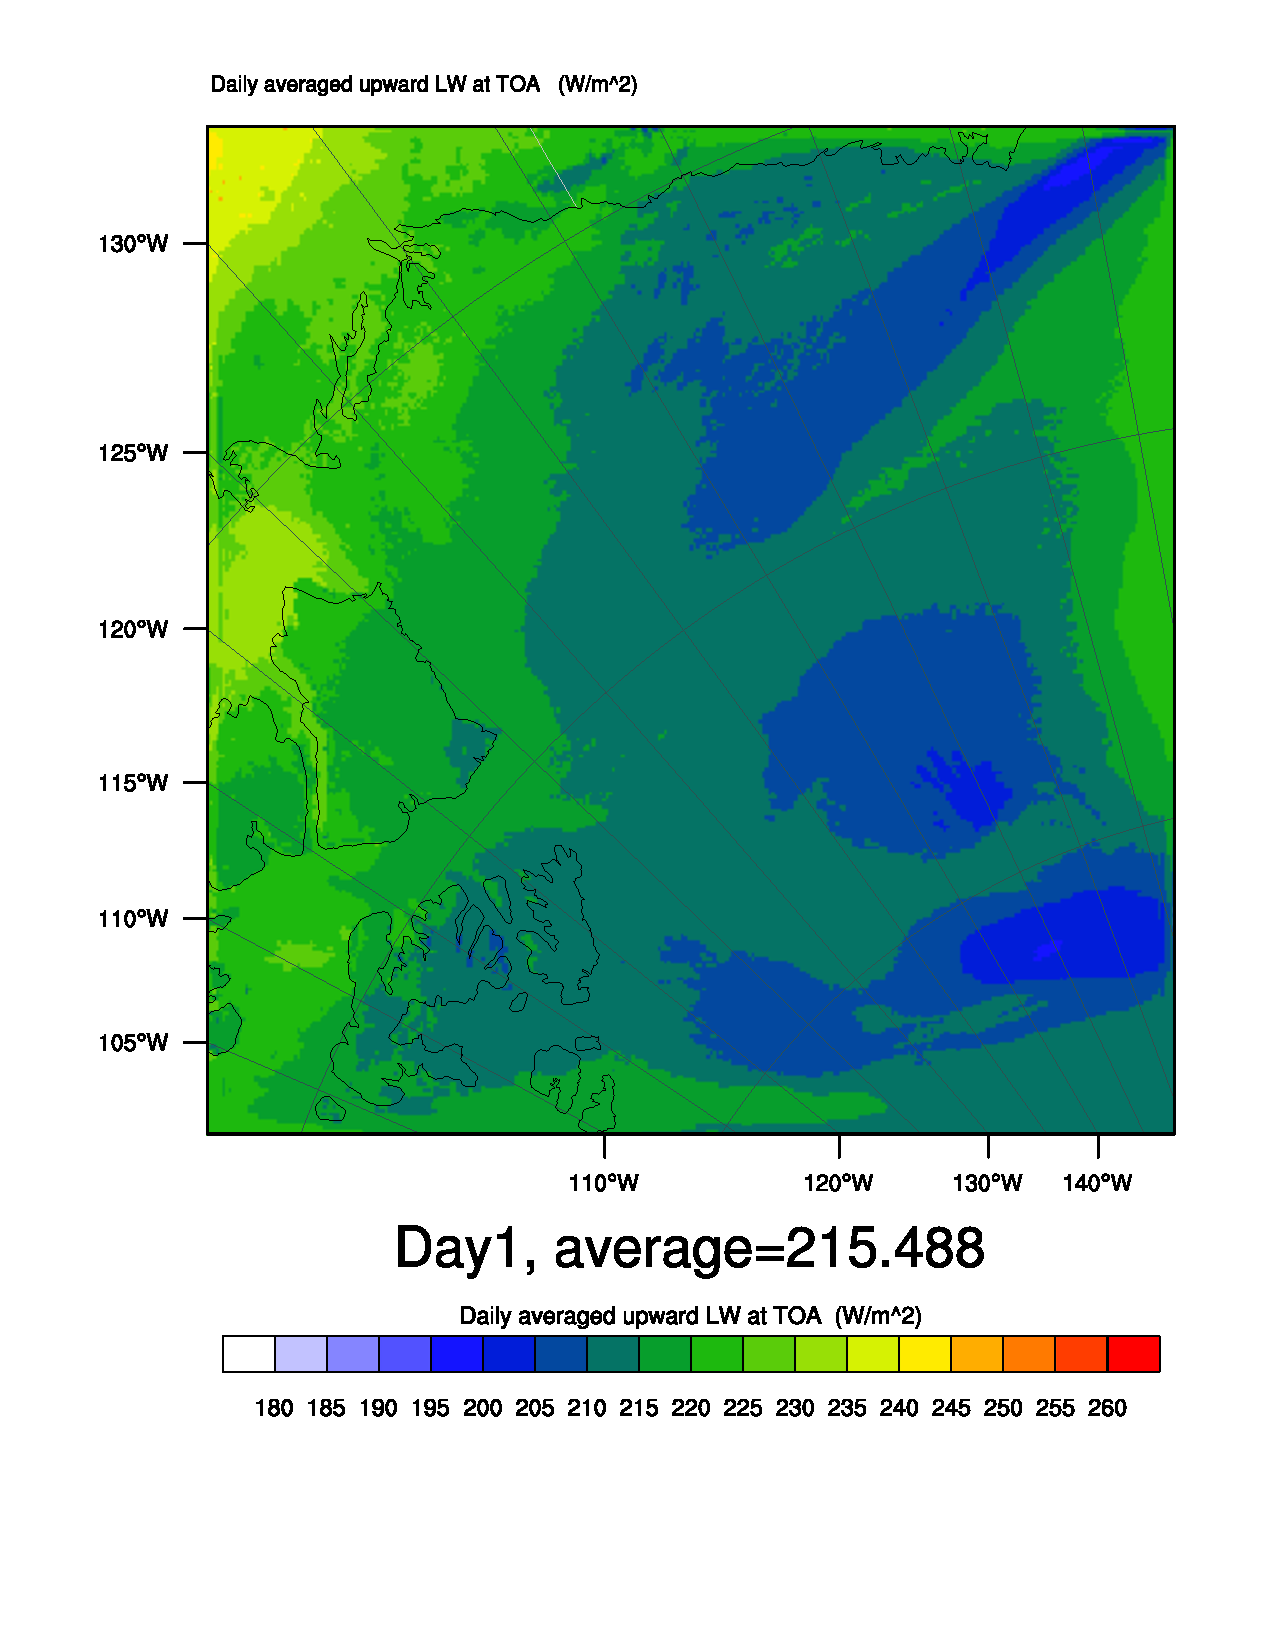
\includegraphics[width=\textwidth]{results/control/LWUPT_Day1.pdf}
		\caption{LW up at TOA, day 1.}
		\label{subfig:lwup_r1Day1}
	\end{subfigure}
	\caption{The average SW and LW flux down at the surface and up at TOA, for day 1. Control. \\Notice the different scales.}
	\label{fig:radiation_r1Day1}
\end{figure}

On day 5, similarly to day 1, the low cloud pattern, illustrated by LWP (figure~\ref{subfig:LWPr1Day5}) is evident in the lack of downward SW at the surface (figure~\ref{subfig:swdown_r1Day5}). The same goes for SW up at TOA (figure~\ref{subfig:swup_r1Day5}), also here the low cloud pattern is recognized. Especially in the area with high LWP (figure~\ref{subfig:LWPr1Day5}) and higher CDNC (figure~\ref{subfig:cdnc_cont_Day5}), 75-72$\degree$N 130-160$\degree$W, the SW flux up at TOA is particulariy high. Assuming that this is reflected by the low clouds in that area fits with equation~\ref{eqn:cloudtau} where the high liquid water path gives a higher cloud optical depth, which in turn gives a high cloud albedo (equation~\ref{eqn:cloudalbedo}). Notice also that both the SW down at the surface (figure~\ref{subfig:swdown_r1Day5}) and up at TOA (figure~\ref{subfig:swup_r1Day5}) is about 110~$\text{W/m}^2$ (notice the different scales) around 75-77$\degree$N and 110-125$\degree$W, and can be seen as small yellow dots in figure~\ref{subfig:swup_r1Day5}. That the flux is almost the same both down at the surface and up at TOA indicates that there are glaciers and/or snow in those spots, with particularly high albedo (0.9-1)~\citep{NSIDC}.

The downward LW at the surface on day 5 (figure~\ref{subfig:glw_r1Day5}) is clearly mostly from the low cloud amounts in the area of 75-72$\degree$N 130-160$\degree$W, which is where the most of the high flux of LW is located. There is also a significant LW signal from the clouds located at 78$\degree$N 120-125$\degree$W. Again confirming the cloud emissivity dependence on LWP (equation~\ref{eqn:epsilon_lw}). The upward LW at TOA (figure~\ref{subfig:lwup_r1Day5}) on the other hand is not highest over the area of highest LWP in the lower layers. The highest flux of LW up at TOA is over Canada in the southernmost part of the study area (south of 70$\degree$N between 130 and 140$\degree$W). This area was free of low clouds (see figure~\ref{subfig:LWPr1Day5}) and is clearly quite free of high clouds too with these high values of LW flux upward at TOA ($\sim$250~$\text{W/m}^2$). The lower values over the area with significantly higher LWP (75-72$\degree$N 130-160$\degree$W) is either because the clouds in that area stretch higher up into the atmosphere, thus emitting at lower temperatures than the low clouds. Following Stefan-Boltzmann's law (equation~\ref{eqn:stefanboltzmann}) yielding a lower emittance of LW flux, or there are simply other clouds higher up in the same area that also would emit less as a consequence of lower temperatures.

%----- Radiation Day5
\begin{figure}
\centering
	\begin{subfigure}{0.48\textwidth}
		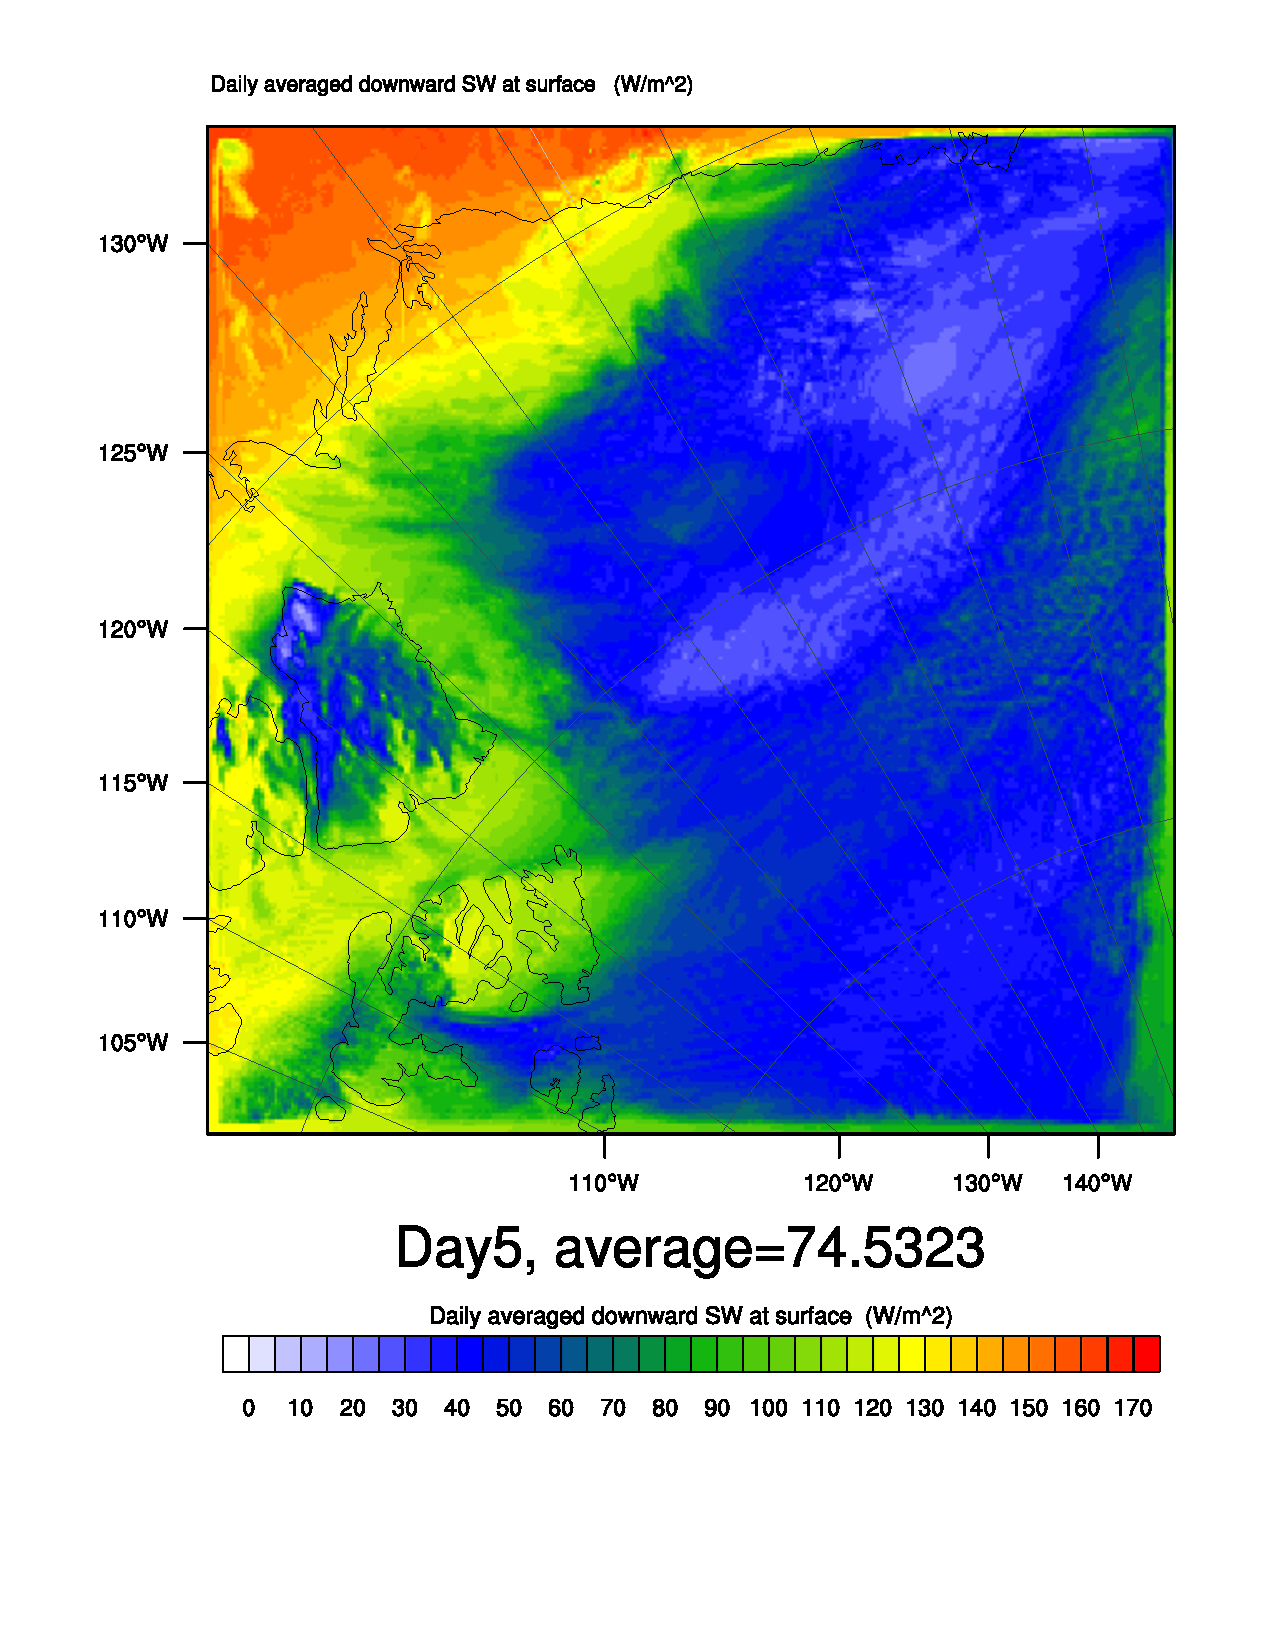
\includegraphics[width=\textwidth]{results/control/SWDOWN_Day5.pdf}
		\caption{SW down at the surface, day 5.}
		\label{subfig:swdown_r1Day5}
	\end{subfigure}
	\quad
	\begin{subfigure}{0.48\textwidth}
		\centering
		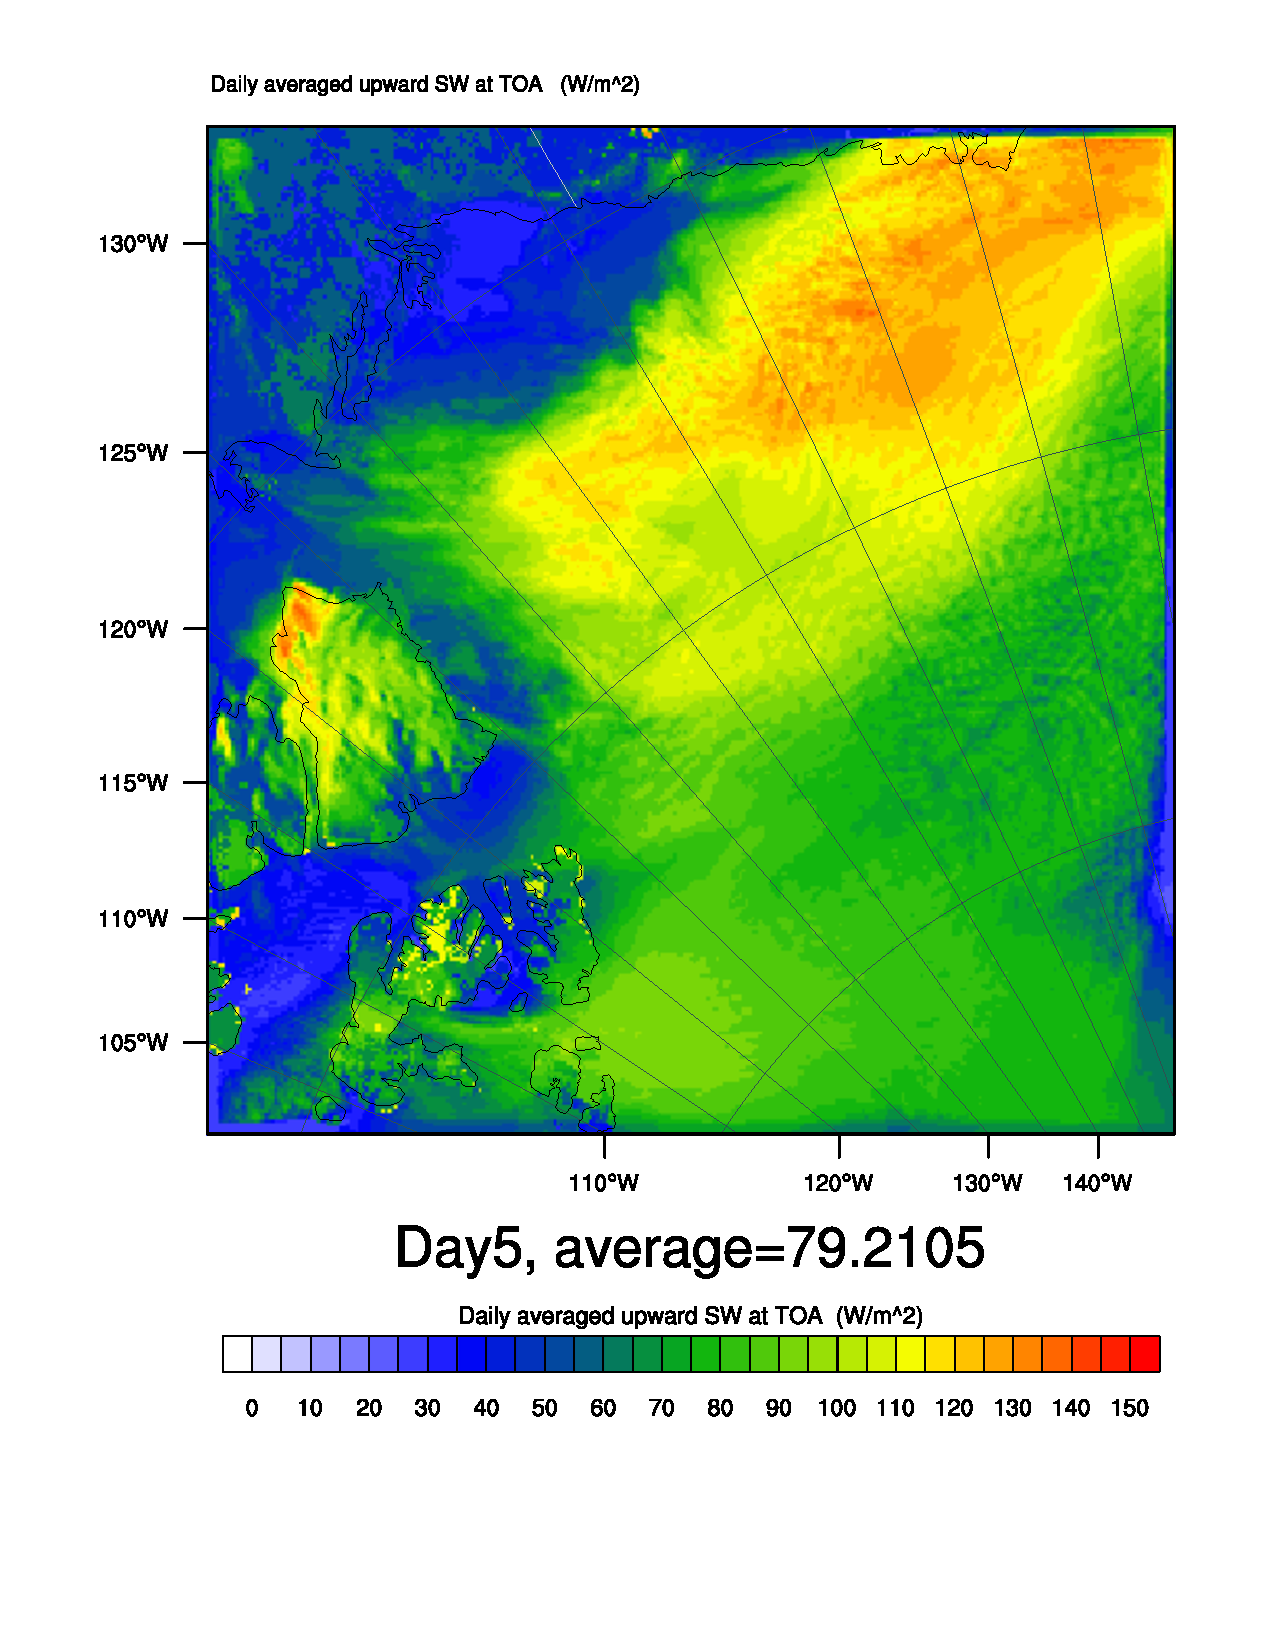
\includegraphics[width=\textwidth]{results/control/SWUPT_Day5.pdf}
		\caption{SW up at TOA, day 5.}
		\label{subfig:swup_r1Day5}
	\end{subfigure}
	
	\begin{subfigure}{0.48\textwidth}
		\centering
		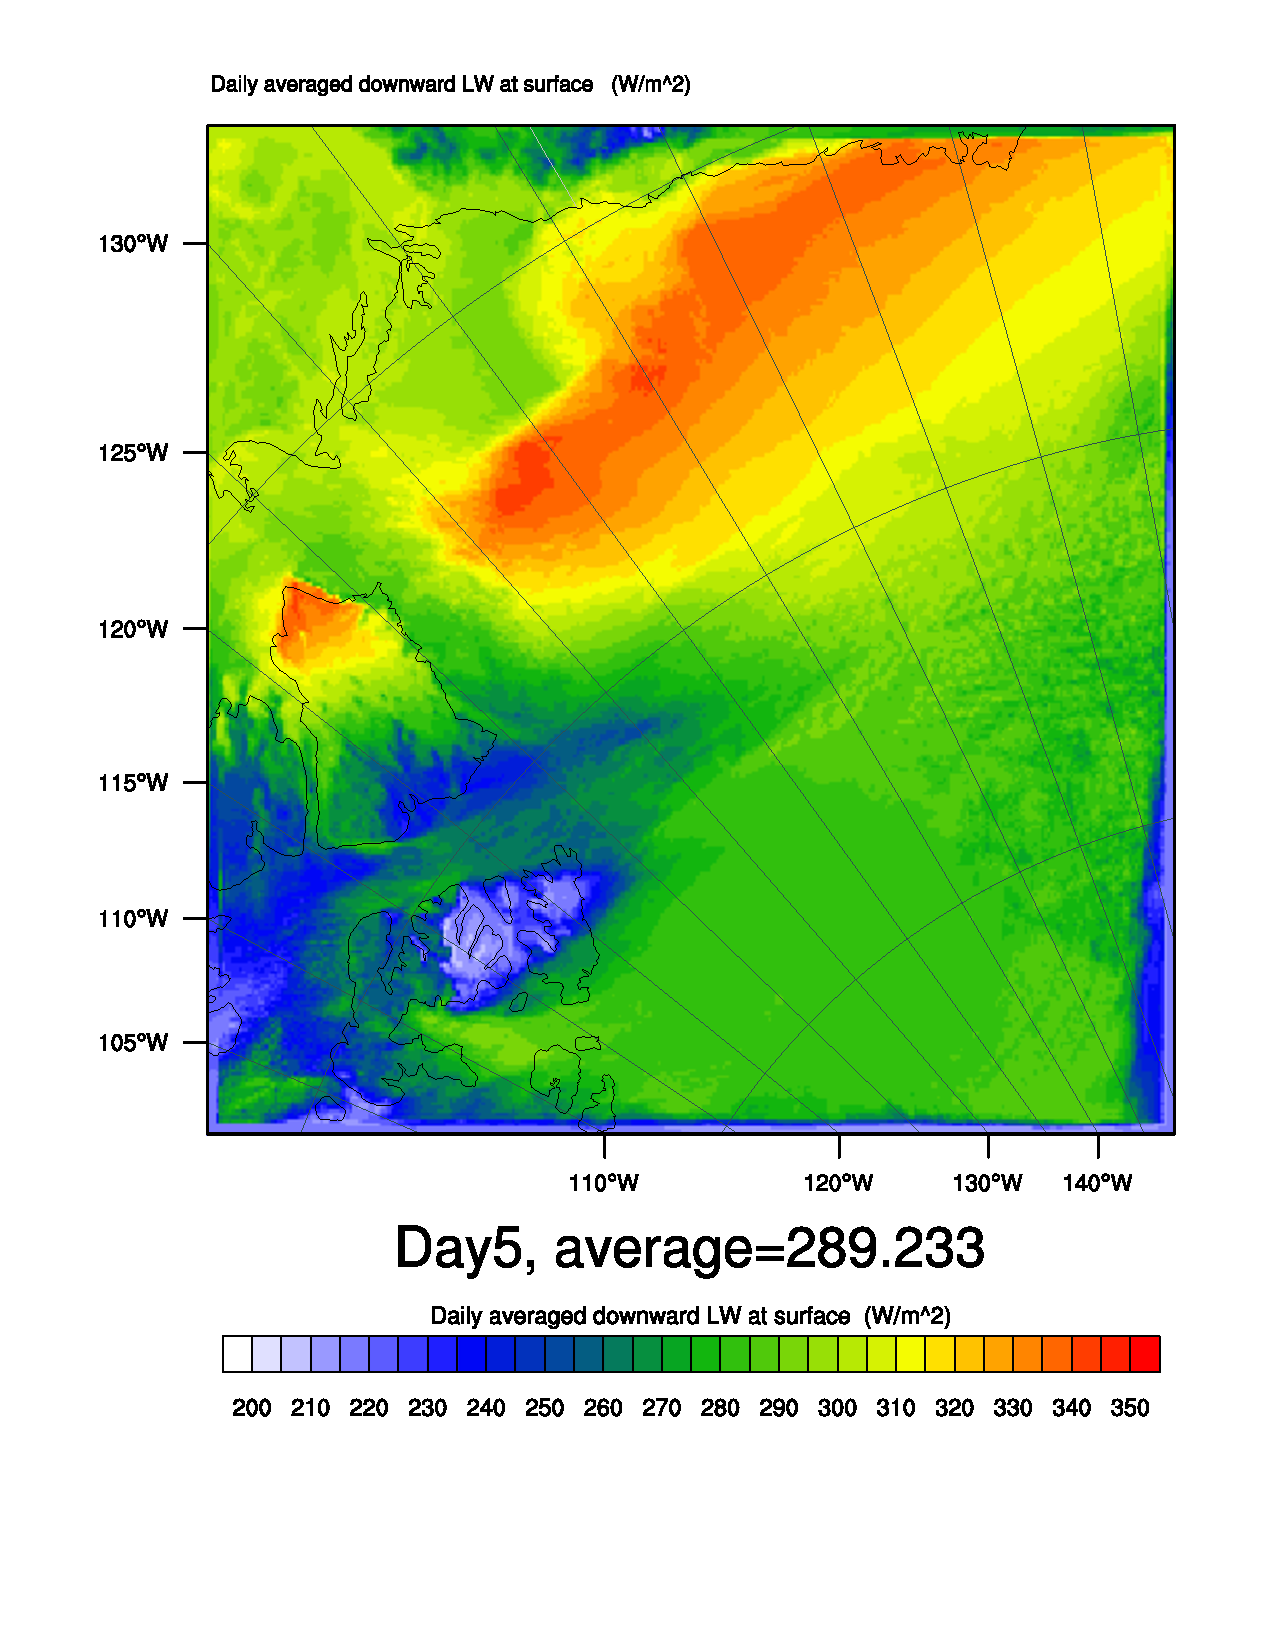
\includegraphics[width=\textwidth]{results/control/GLW_Day5.pdf}
		\caption{LW down at the surface, day 5.}
		\label{subfig:glw_r1Day5}
	\end{subfigure}
	\quad
	\begin{subfigure}{0.48\textwidth}
		\centering
		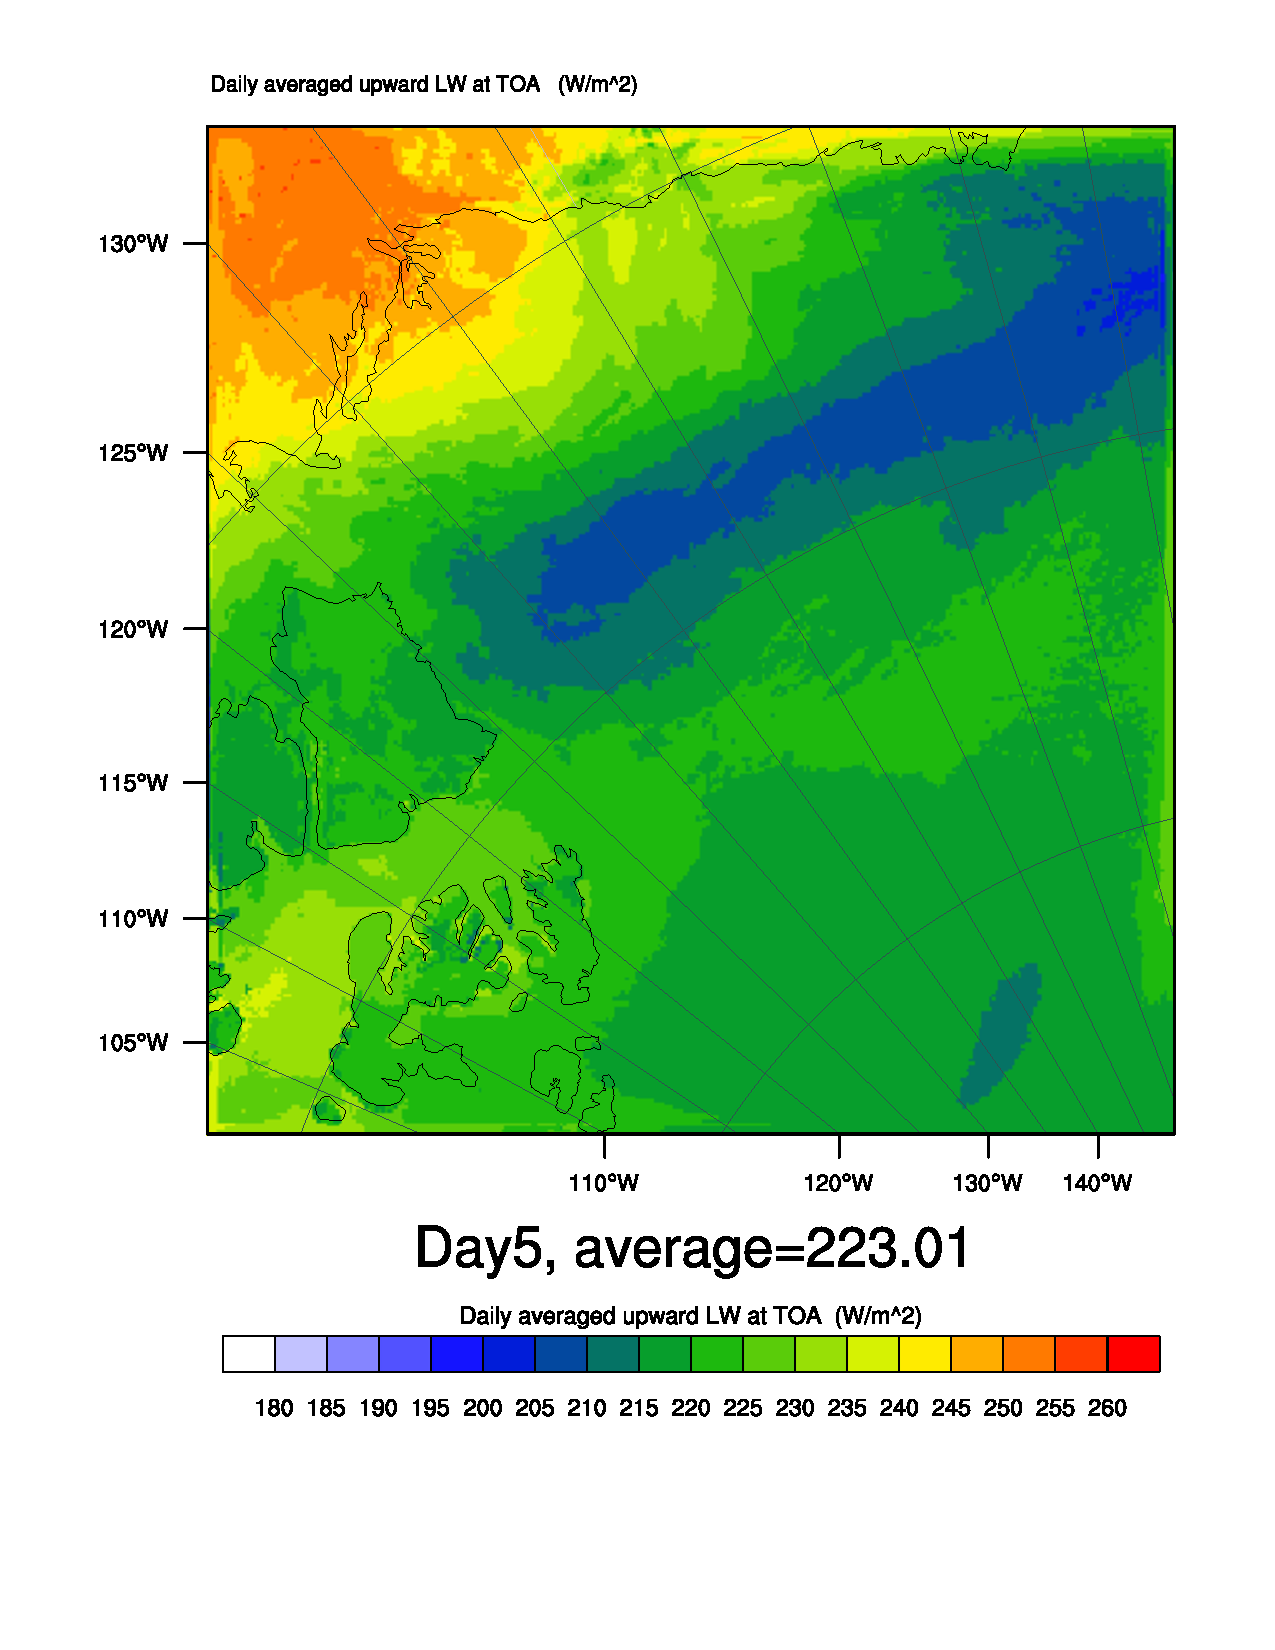
\includegraphics[width=\textwidth]{results/control/LWUPT_Day5.pdf}
		\caption{LW up at TOA, day 5.}
		\label{subfig:lwup_r1Day5}
	\end{subfigure}
	\caption{The average SW and LW flux down at the surface and up at TOA, for day 5. Control.\\Notice the different scales.}
	\label{fig:radiation_r1Day5}
\end{figure}

The heat fluxes upward at the surface, latent heat (LH) and sensible heat (SH), are also of interest when studying clouds in the Arctic. The fluxes are shown in figure~\ref{fig:surface_fluxes_r1} for days 1 and 5. Notice that the LH is lower over the sea ice for both days 1 and 5. This because the sea ice is colder than the ocean, and works as a lid over that part of the ocean, not letting all the heat and water vapor out. Another thing to notice is the marked increase in SH just off the sea ice edge, 77$\degree$N, 135$\degree$W, day 5. This is due to the strong winds in that area (figure~\ref{subfig:weather_cont_day5}), which brings cold air from over the ice out over the warmer open ocean. Thus the temperature gradient is stronger just off the sea ice edge, increasing the heat given from the surface to the overlying air. The effect is strongest at the sea ice edge, but is also evident further away over the ocean, to about 160$\degree$W. The reason the signal is so clear at the ice edge and stretches far is the wind speed, which is just above 10~$\text{m/s}$ (see figure~\ref{subfig:weather_cont_day5}). In figure~\ref{subfig:sh_r1Day5} is also a white "blob" south of the sea ice (70-75$\degree$N and 125-140$\degree$W), which indicates a negative heat flux of about 20~$\text{W/m}^2$. There the surface draws heat from the overlying air, since the temperature at 2~m height (figure~\ref{subfig:weather_cont_day5}) is higher than the skin temperature (figure~\ref{subfig:skin_r1Day5}) in that area. This warmer air is brought over the ocean by winds coming from land southeast of that area, see figure~\ref{subfig:weather_cont_day5}. The figure also shows the strength of the wind field, which was mentioned as a reason for the high SH off the ice edge and is also the reason for the strong negative heat flux.

%----- Surface heat fluxes
\begin{figure}
\centering
	\begin{subfigure}{0.48\textwidth}
		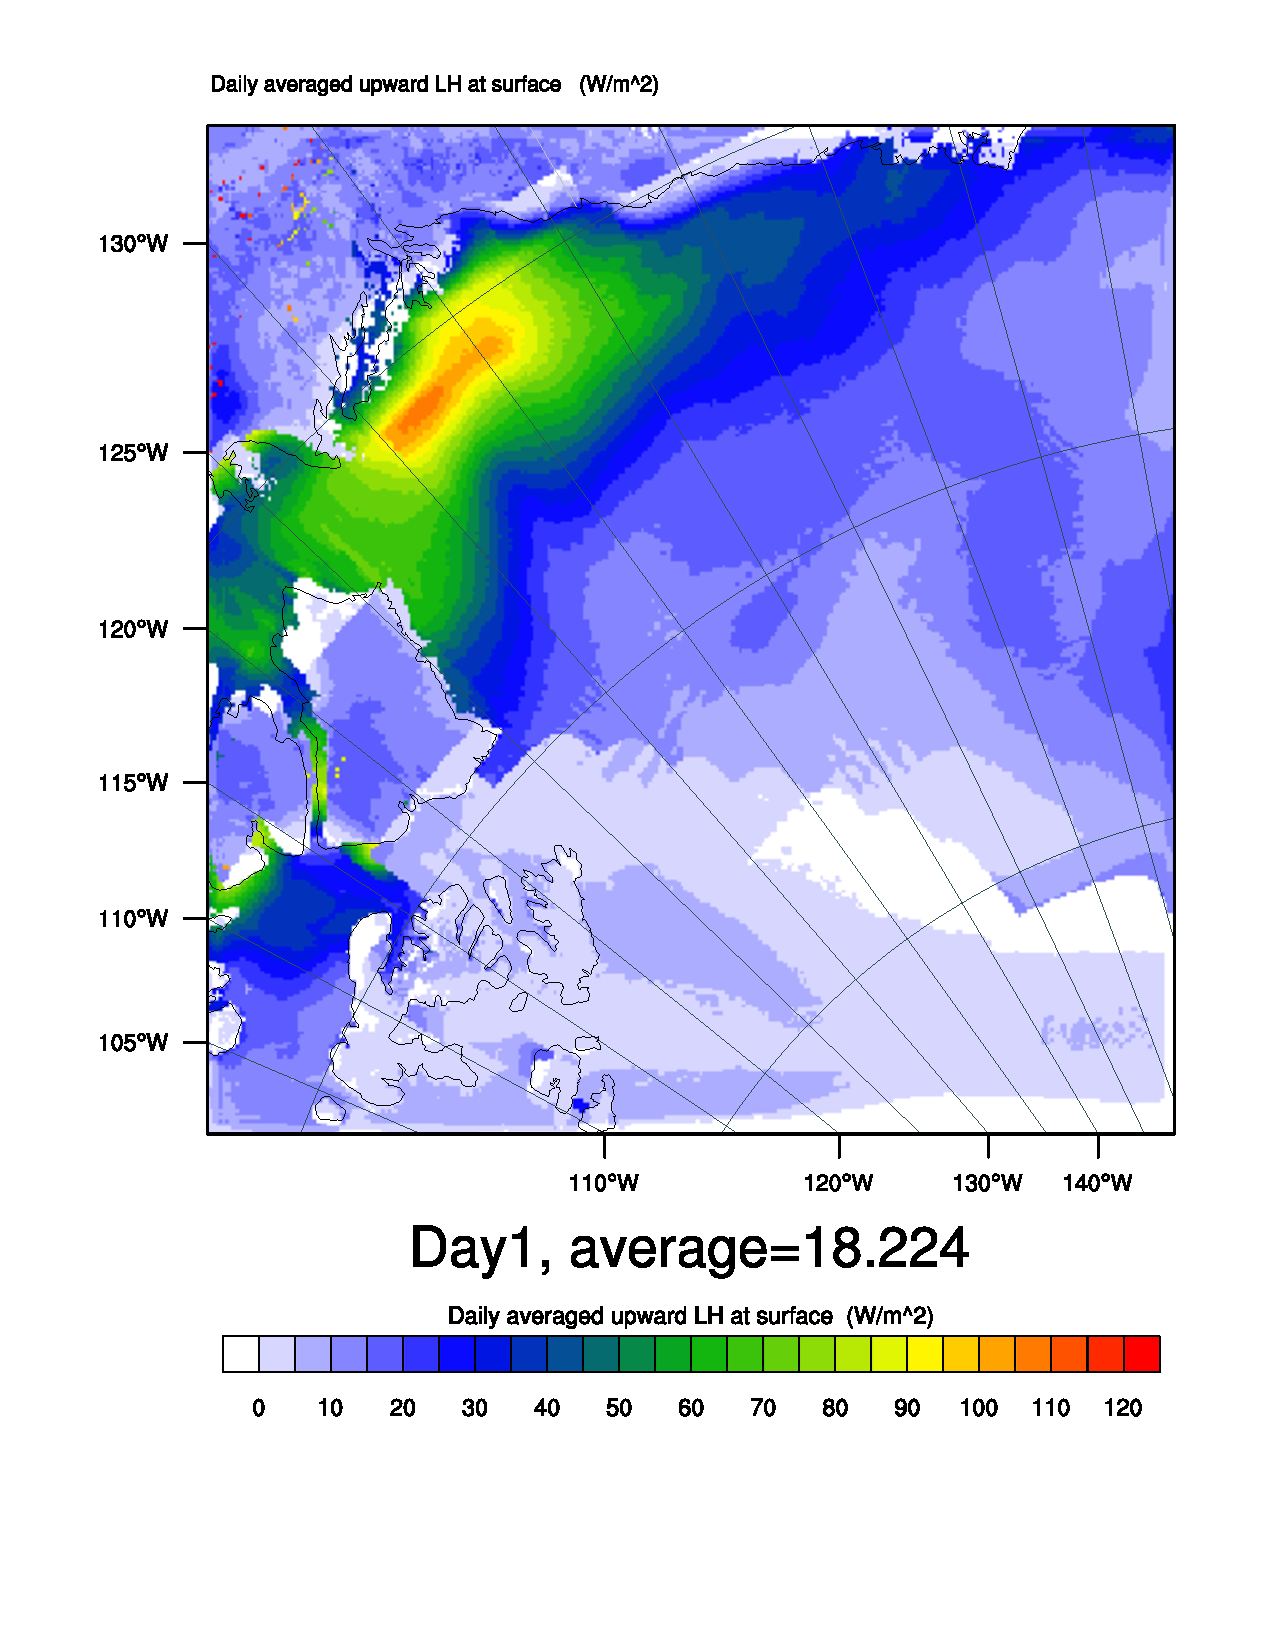
\includegraphics[width=\textwidth]{results/control/LH_Day1.pdf}
		\caption{LH day 1.}
		\label{subfig:lh_r1Day1}
	\end{subfigure}
	\quad
	\begin{subfigure}{0.48\textwidth}
		\centering
		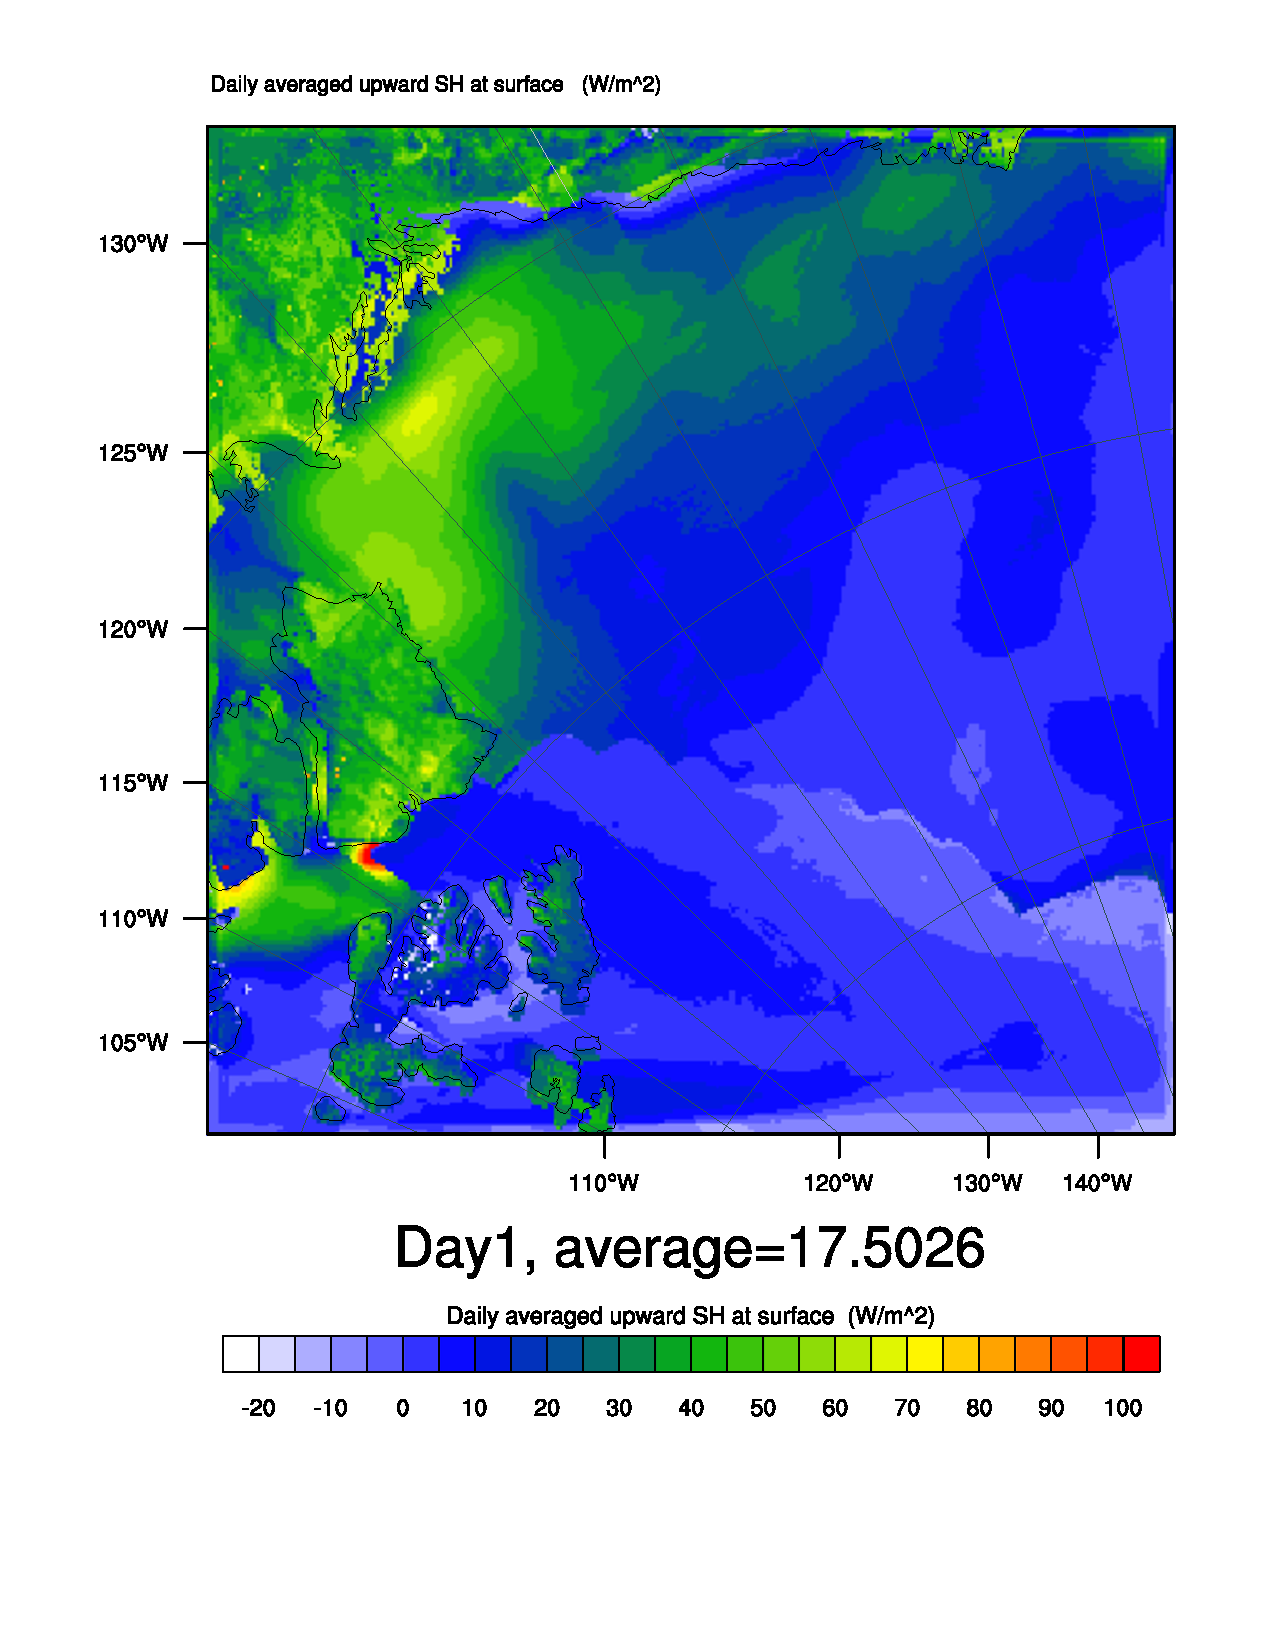
\includegraphics[width=\textwidth]{results/control/HFX_Day1.pdf}
		\caption{SH day 1.}
		\label{subfig:sh_r1Day1}
	\end{subfigure}
	
	\begin{subfigure}{0.48\textwidth}
		\centering
		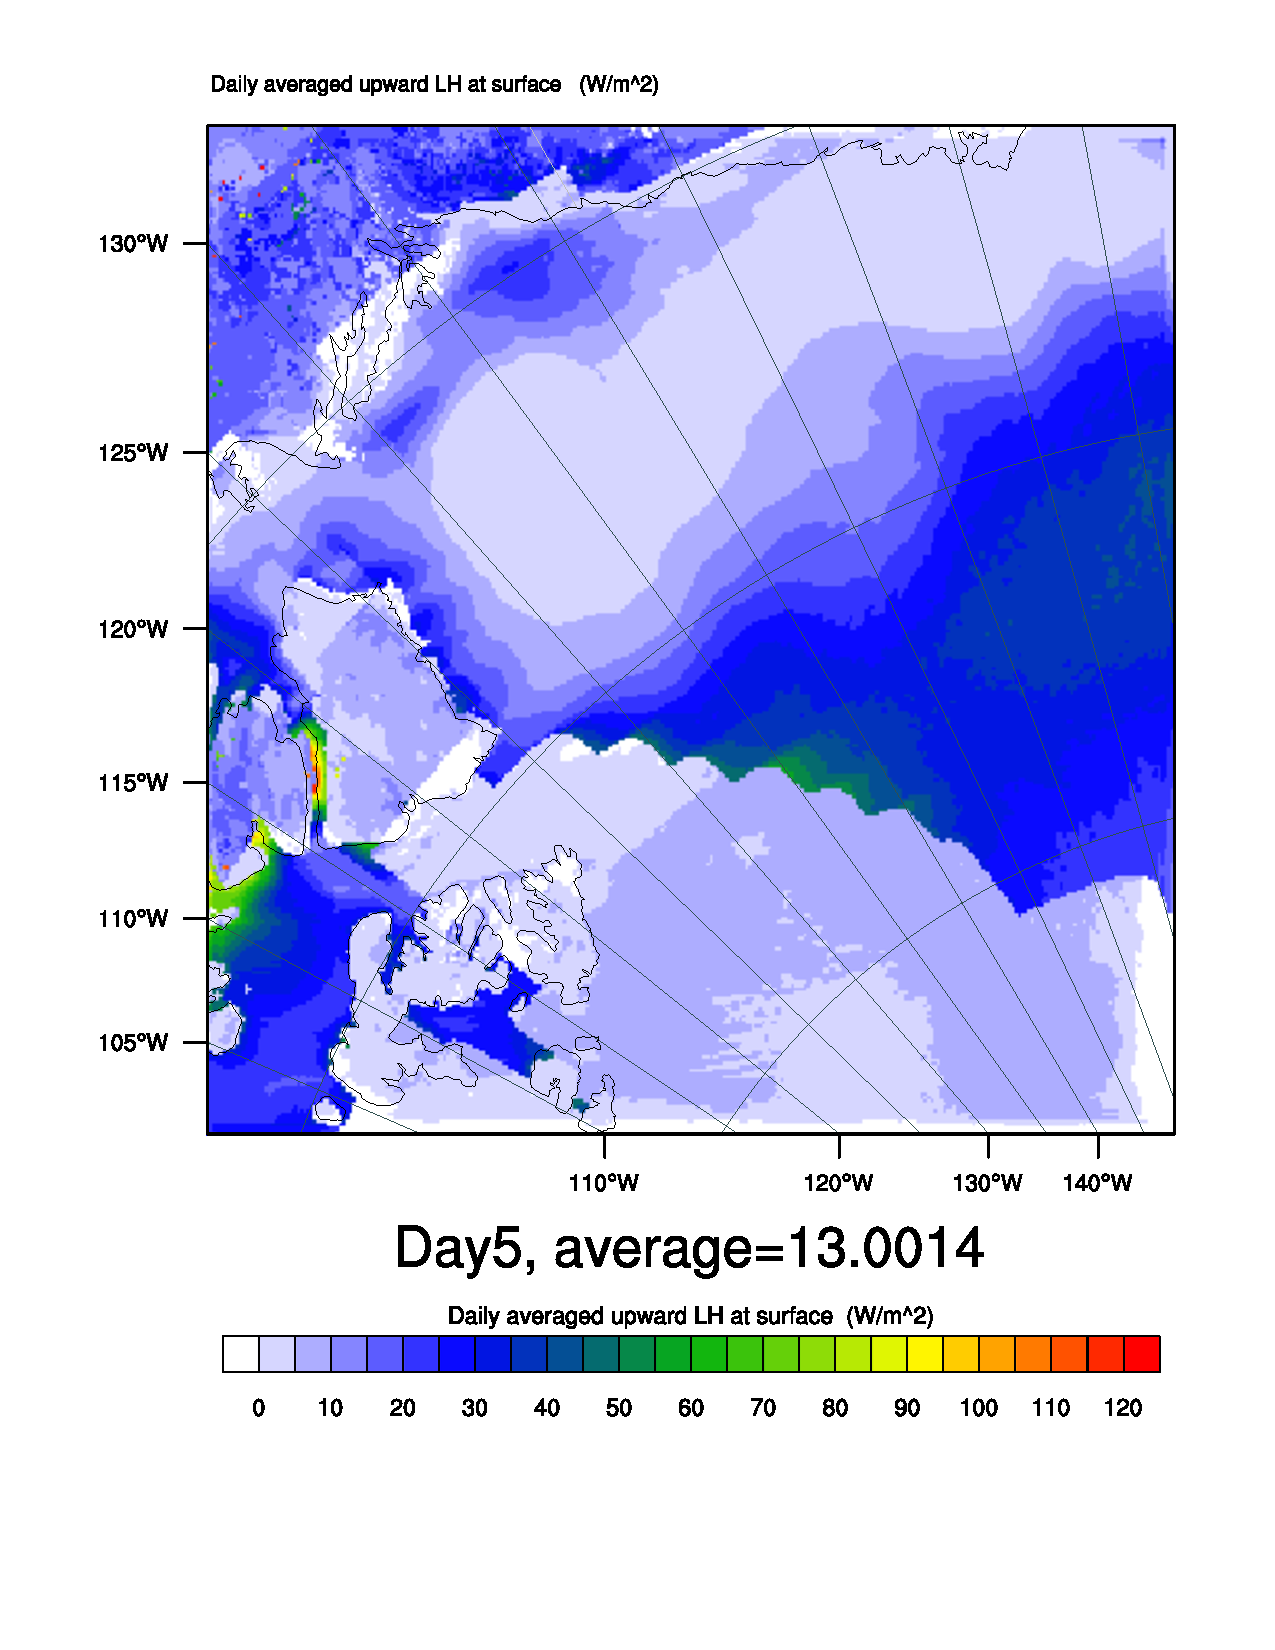
\includegraphics[width=\textwidth]{results/control/LH_Day5.pdf}
		\caption{LH day 5.}
		\label{subfig:lh_r1Day5}
	\end{subfigure}
	\quad
	\begin{subfigure}{0.48\textwidth}
		\centering
		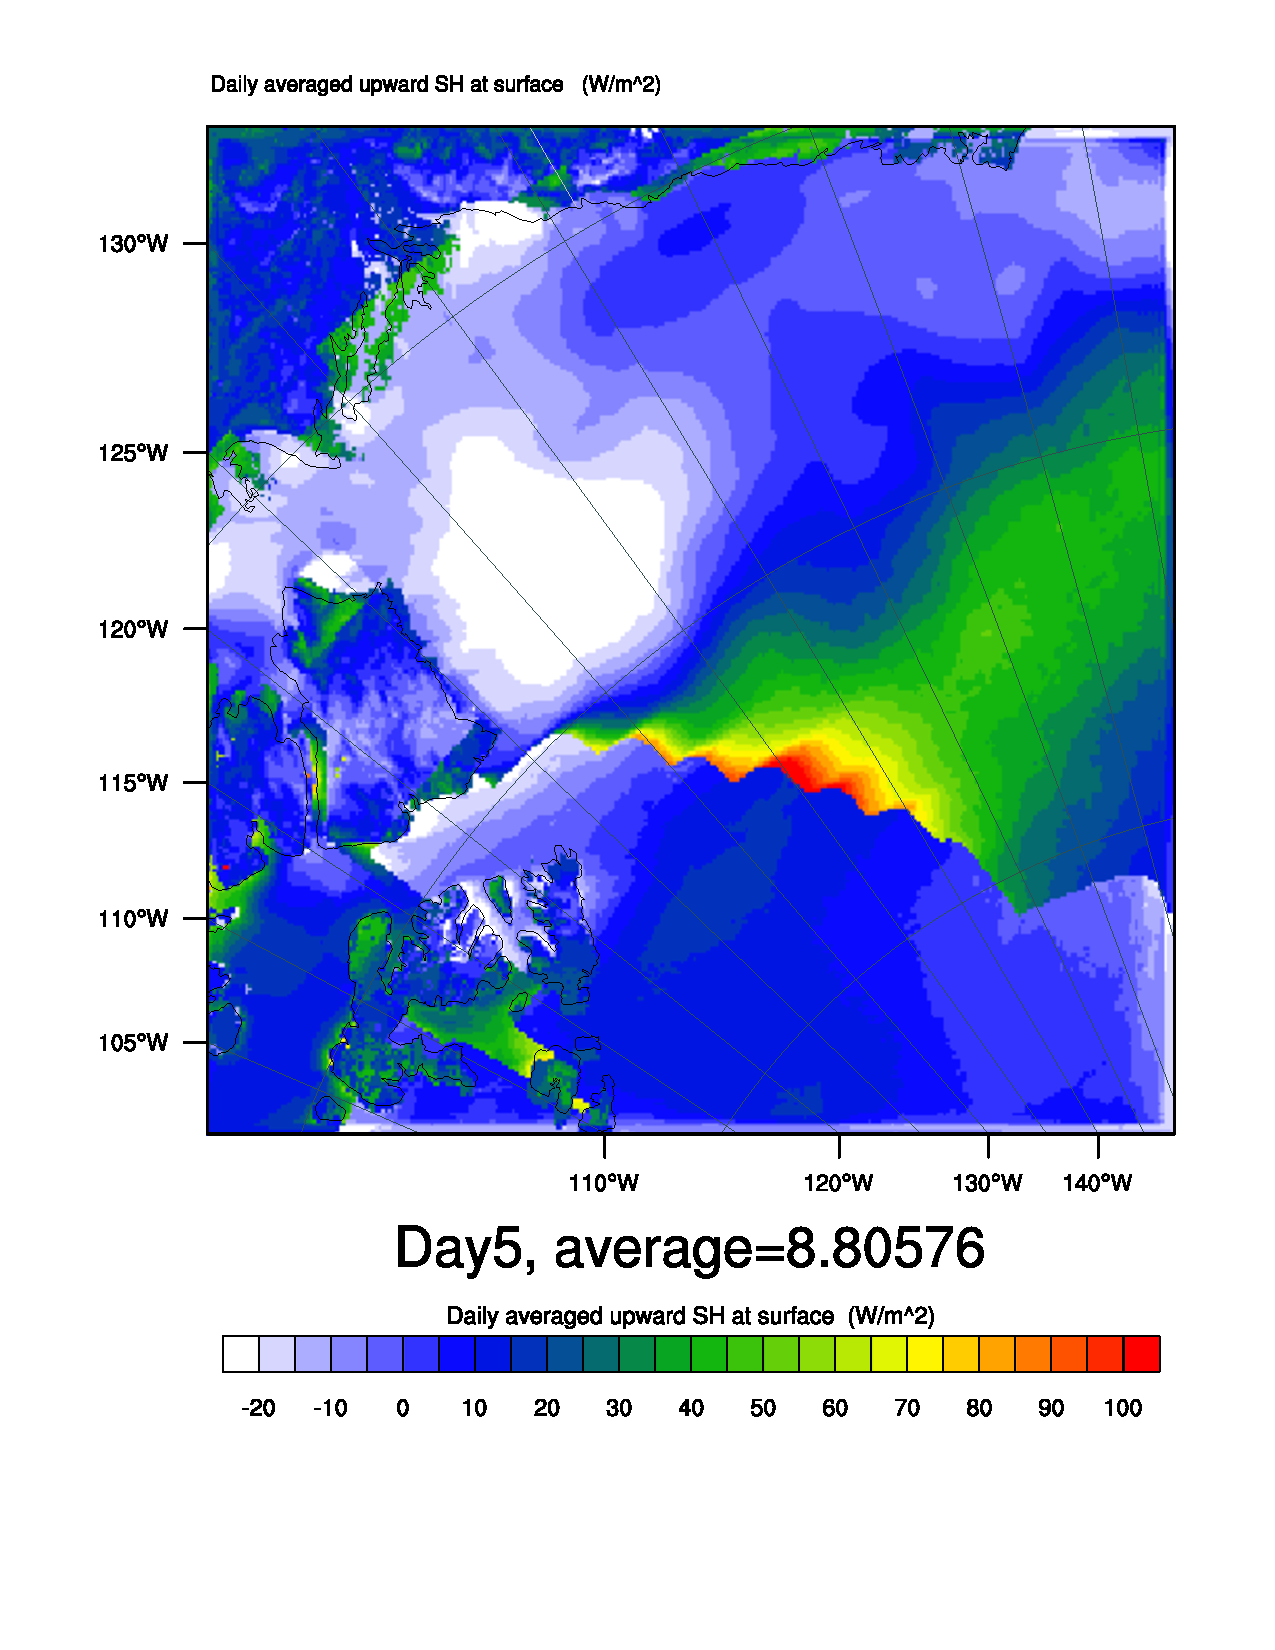
\includegraphics[width=\textwidth]{results/control/HFX_Day5.pdf}
		\caption{SH day 5.}
		\label{subfig:sh_r1Day5}
	\end{subfigure}
	\caption{The average surface heat fluxes (SH and LH) up at the surface, for days 1 and 5. Control.}
	\label{fig:surface_fluxes_r1}
\end{figure}

The daily time averaged skin temperature of the study area is shown in figure~\ref{fig:skintemp}, for both days. It shows that the skin temperature is generally lower at the sea ice surface, than the ocean surface and land surfaces. Also, the skin temperature increases further south, and is highest over land, which is furthest south. The skin temperature is lowest in day 5, in those same spots that were claimed to be glacier and/or snow when discussing the figures showing SW down at the surface and up at TOA on day 5 (figures~\ref{subfig:swdown_r1Day5} and~\ref{subfig:swup_r1Day5}). The temperature there is $\sim$-13$\degree$C (260~K).
%--------- Skin temperature
\begin{figure}
	\begin{subfigure}{0.48\textwidth}
		\centering
		\includegraphics[width=\textwidth]{results/control/skintemp_day1.pdf}
		\caption{Day 1}
		\label{subfig:skin_r1Day1}
	\end{subfigure}
	\begin{subfigure}{0.48\textwidth}
		\centering
		\includegraphics[width=\textwidth]{results/control/skintemp_day5.pdf}
		\caption{Day 5}
		\label{subfig:skin_r1Day5}
	\end{subfigure}
	\caption{Daily averaged skin temperature (K) of the study area, for both days 1 and 5. Control.\\Notice the different scales.}
	\label{fig:skintemp}
\end{figure}

%-------------------------------
\clearpage
\section{Removed sea ice}
%-------------------------------
The sea ice was removed to study the effect this had on the cloud radiative properties, and through that if it had heating or cooling effects at the surface. The sea ice that was present in the control run, but has been removed for NoIce, is shown in figure~\ref{fig:seaice}. 

\begin{figure}[hb]
\centering
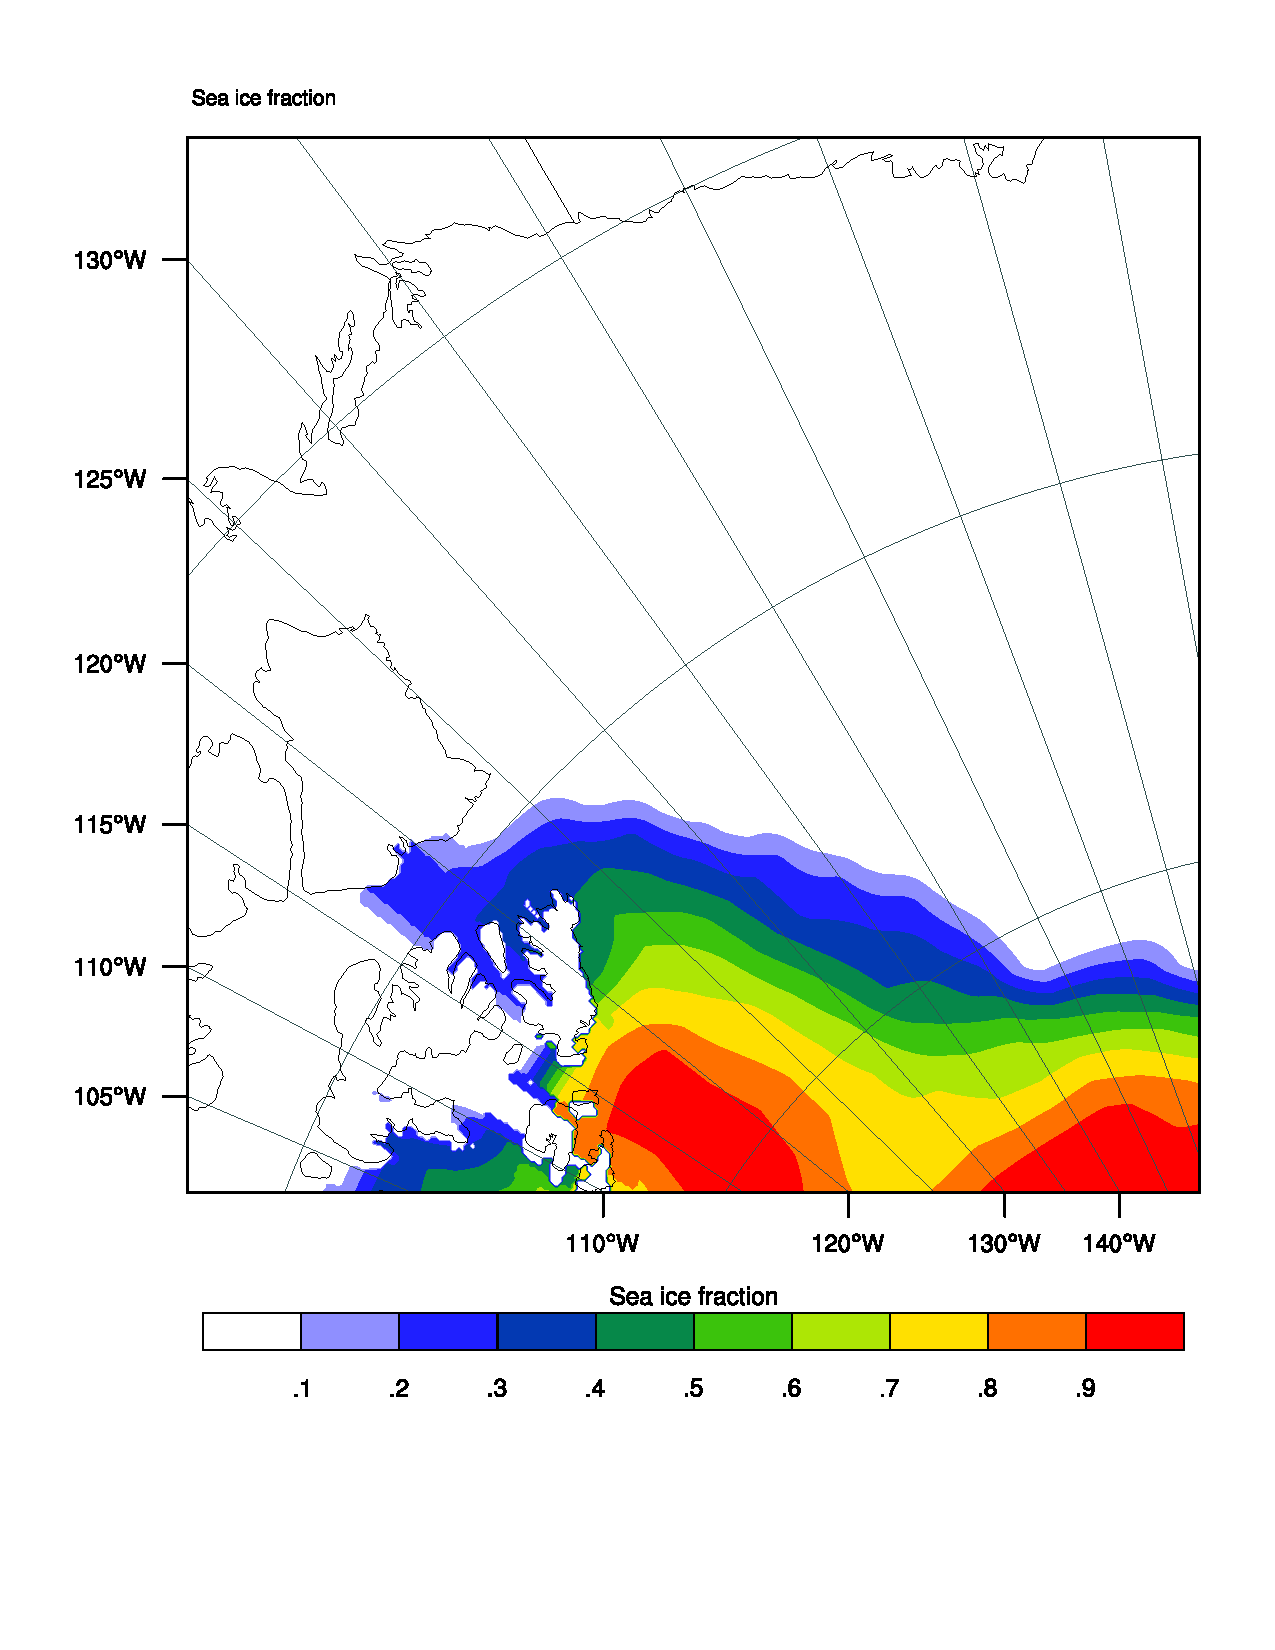
\includegraphics[width=0.5\textwidth]{results/control/seaiceplot.pdf}
\caption{Sea ice fraction in Control (and Aero10).}
\label{fig:seaice}
\end{figure}

\subsection{Day 1}
\label{sec:noiceDay1}
Removal of sea ice should lead to an increase in aerosol number concentration. As mentioned in Chapter~\ref{chap:introduction}, the open sea surface will release sea salt, primary organic matter and DMS. The increase in water-friendly aerosols is seen just over the newly open sea surface in figure~\ref{subfig:aerocrossQNWFA}. Recall that the section is over the red line shown in figure~\ref{subfig:cross_line}, over the sea ice. Making the same approximation here as for CDNC, $10^6~\text{kg}^{-1}=1~\text{cm}^{-3}$, there is an increase of water-friendly aerosols of up to 25~$\text{cm}^{-3}$. And above there is approximately an equal decrease. Although the numbers in figure~\ref{subfig:aerocrossQNCLOUD}, showing difference in CDNC between NoIce and Control, are not the same, there is an increase in number of droplets in the same area as there is a decrease in water-friendly aersols. This indicates that water-friendly aerosols that were not activated in Control could be activated and grow into cloud droplets in NoIce, due to enhanced evaporation from the open ocean. This meaning that the clouds in the control run (figure~\ref{subfig:cross_LWC_day1}) are there in NoIce too (similar pattern), but get denser where the water-friendly aerosols are now activated. This means that there are more available aerosols close to the newly opened sea surface, and that aerosols in that area are more likely to be activated due to enhanced evaporation.

\begin{figure}[ht]
\centering
	\begin{subfigure}{0.48\textwidth}
		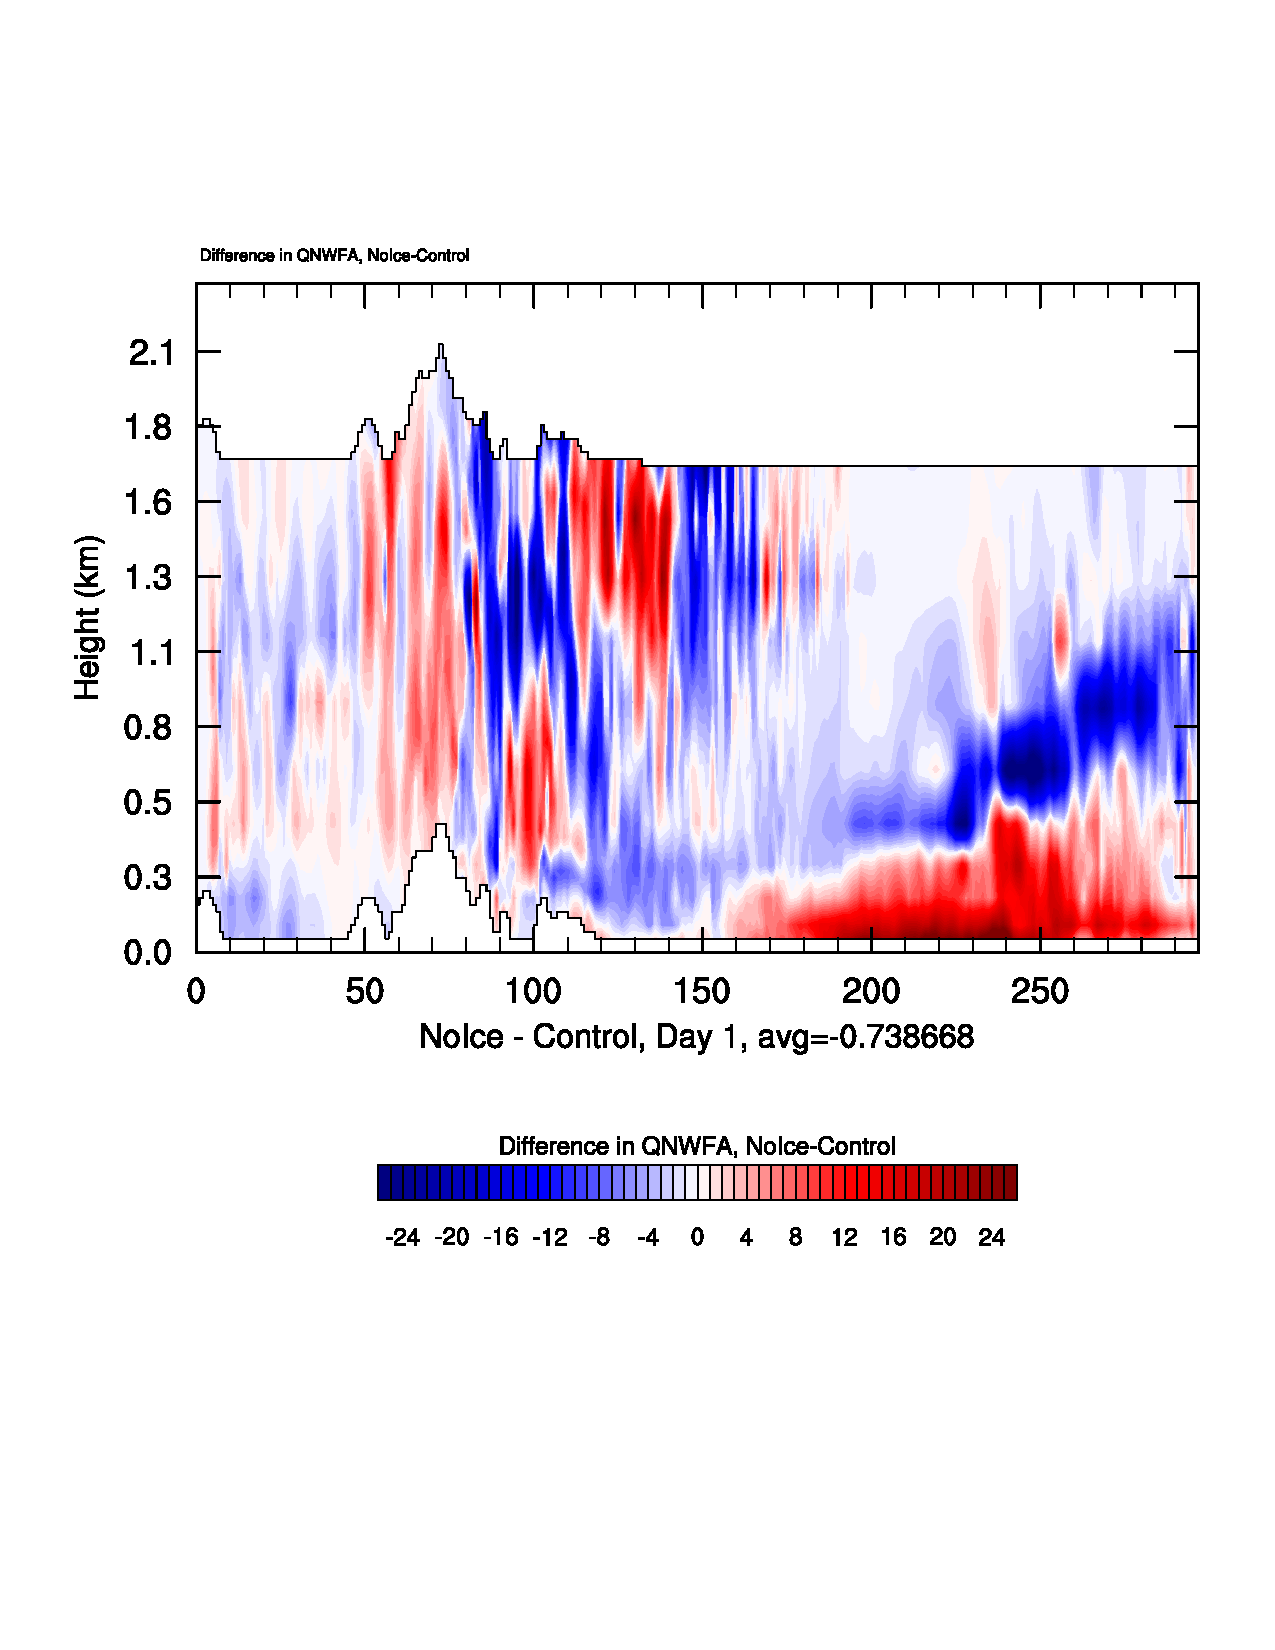
\includegraphics[width=\textwidth]{results/noice/diffSec_QNWFA_NoIce_Day1.pdf}
		\caption{Difference in water-friendly aerosols.}
		\label{subfig:aerocrossQNWFA}
	\end{subfigure}
	\quad
		\begin{subfigure}{0.48\textwidth}
		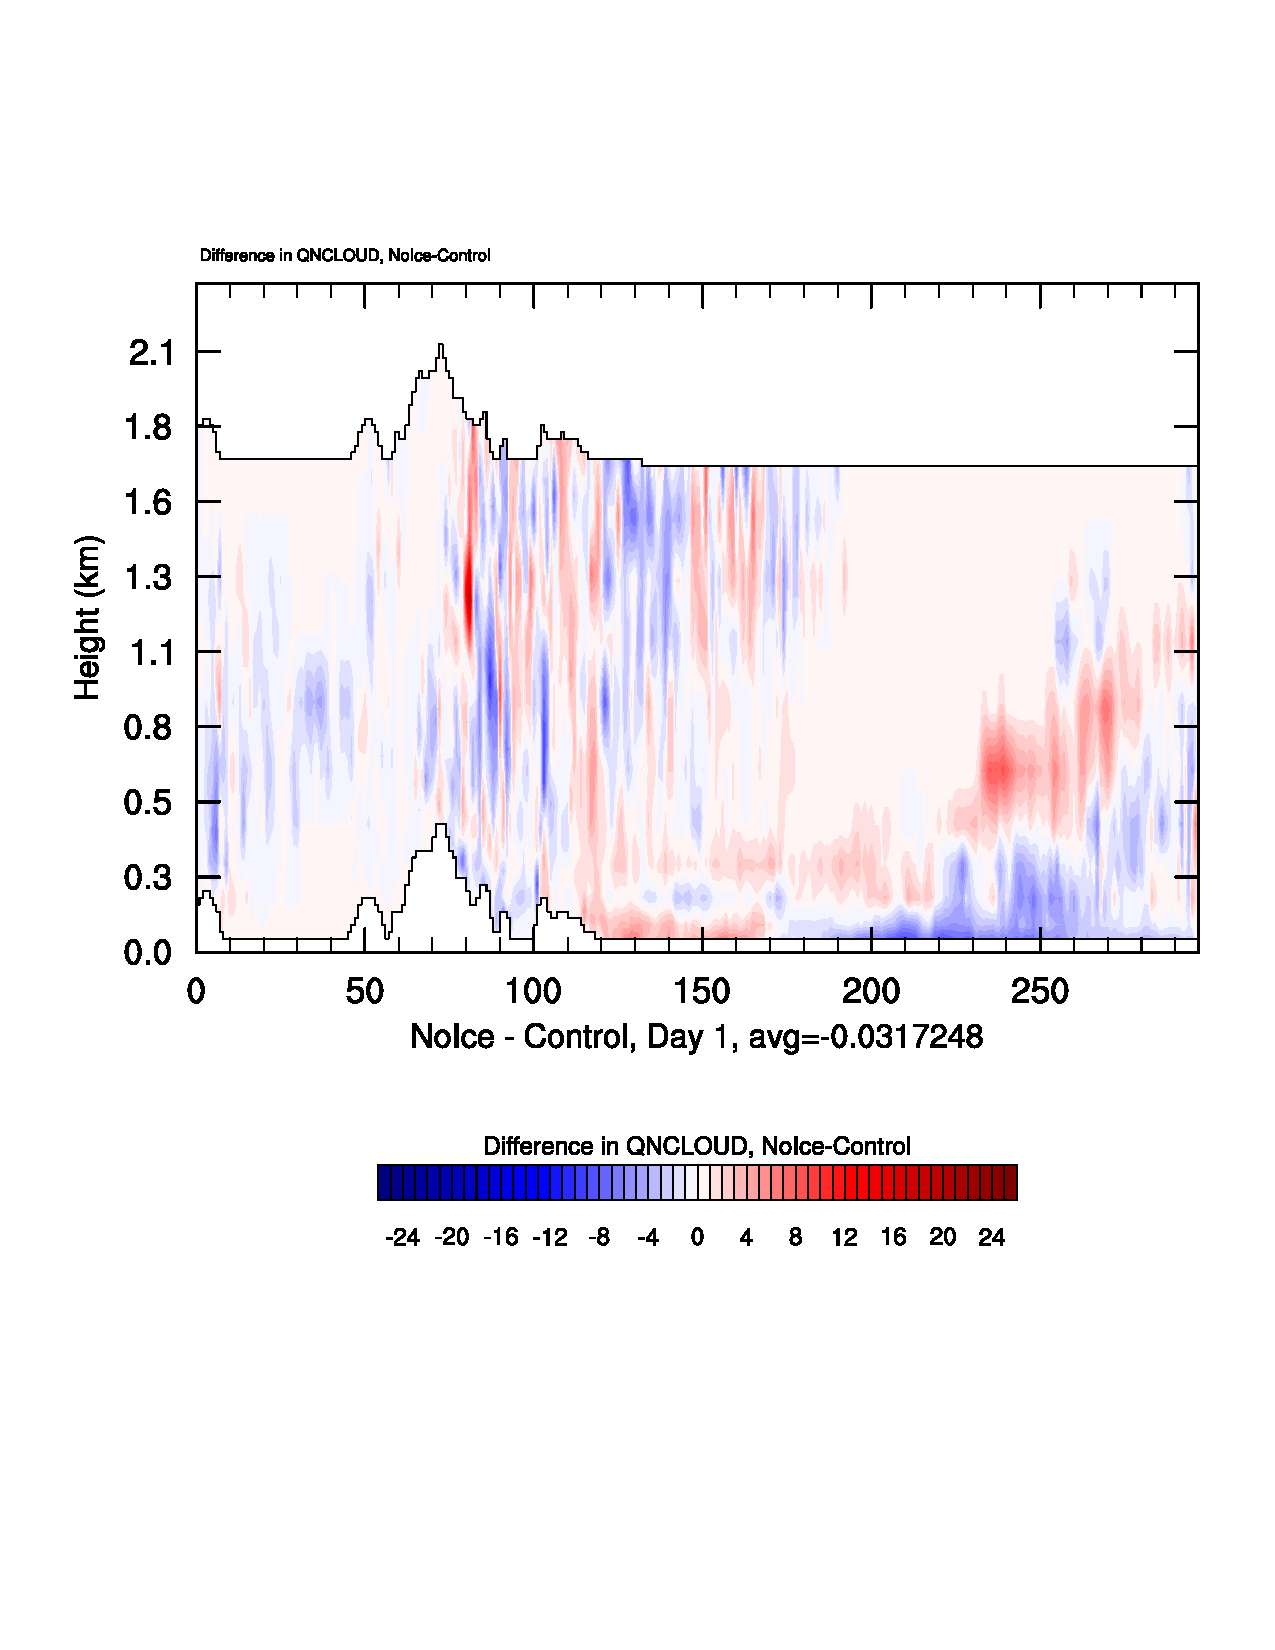
\includegraphics[width=\textwidth]{results/noice/diffSec_QNCLOUD_NoIce_Day1.pdf}
		\caption{Difference in CDNC.}
		\label{subfig:aerocrossQNCLOUD}
	\end{subfigure}
	\caption{Difference in time averaged CDNC and number concentration of water-friendly aerosols for day1. Units: $\text{kg}^{-1}$. NoIce-Control.}
	\label{fig:aeroSections}
\end{figure}

The average difference in LWP, NoIce-Control, for day 1, shown in figure~\ref{subfig:LWPr2Day1} is small for the whole field ($\sim$0.23~$\text{g/m}^2$ increase). But the area of interest in this case is where the sea ice is no longer present (recall figure~\ref{fig:seaice}). The area where there was sea ice in the control run shows a positive difference in LWP. Especially furthest north (bottom right corner of the map) the LWP is significantly higher, >15~$\text{g/m}^2$.

\begin{figure}
\centering
	\begin{subfigure}{0.48	\textwidth}
		\centering
		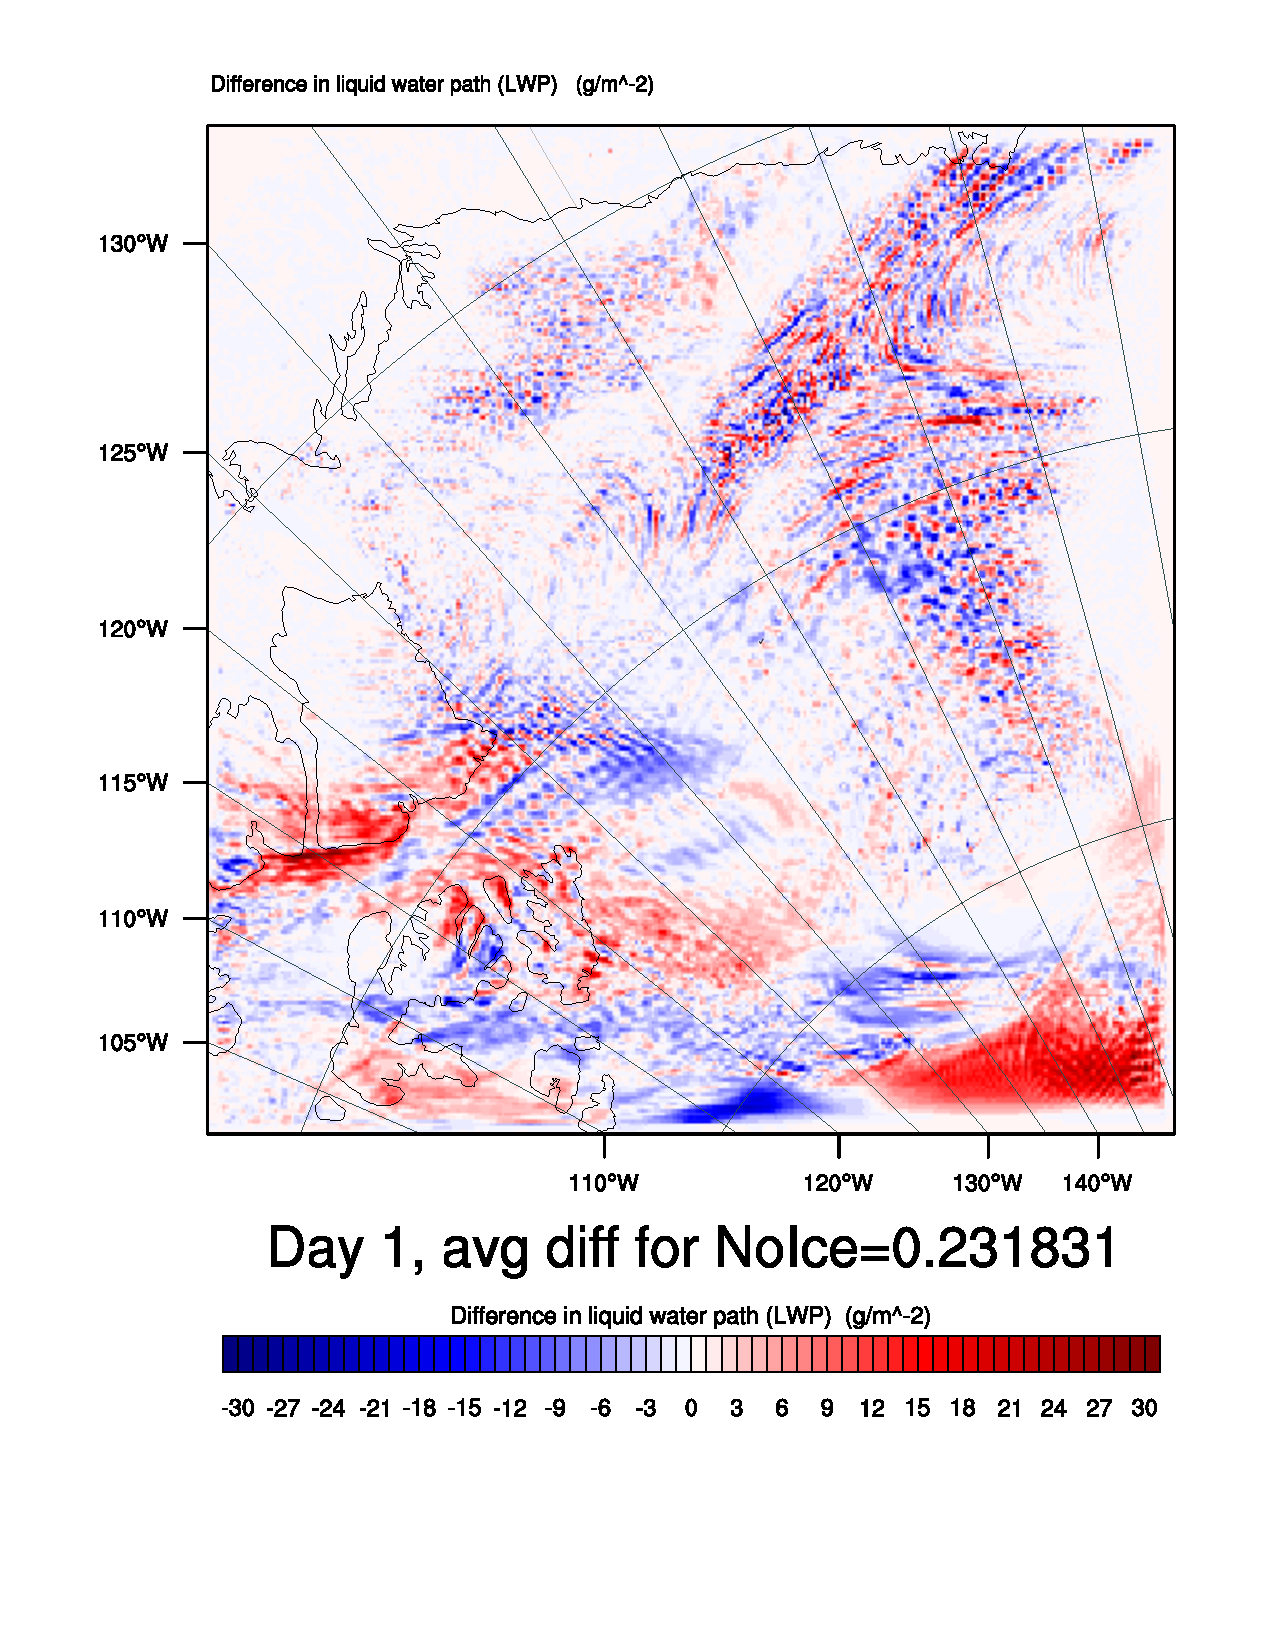
\includegraphics[width=\textwidth]{results/noice/Diff_LWP_Day1NoIce.pdf}
		\caption{LWP, NoIce, day 1}
		\label{subfig:LWPr2Day1}
	\end{subfigure}
	\quad
	\begin{subfigure}{0.48\textwidth}
		\centering
		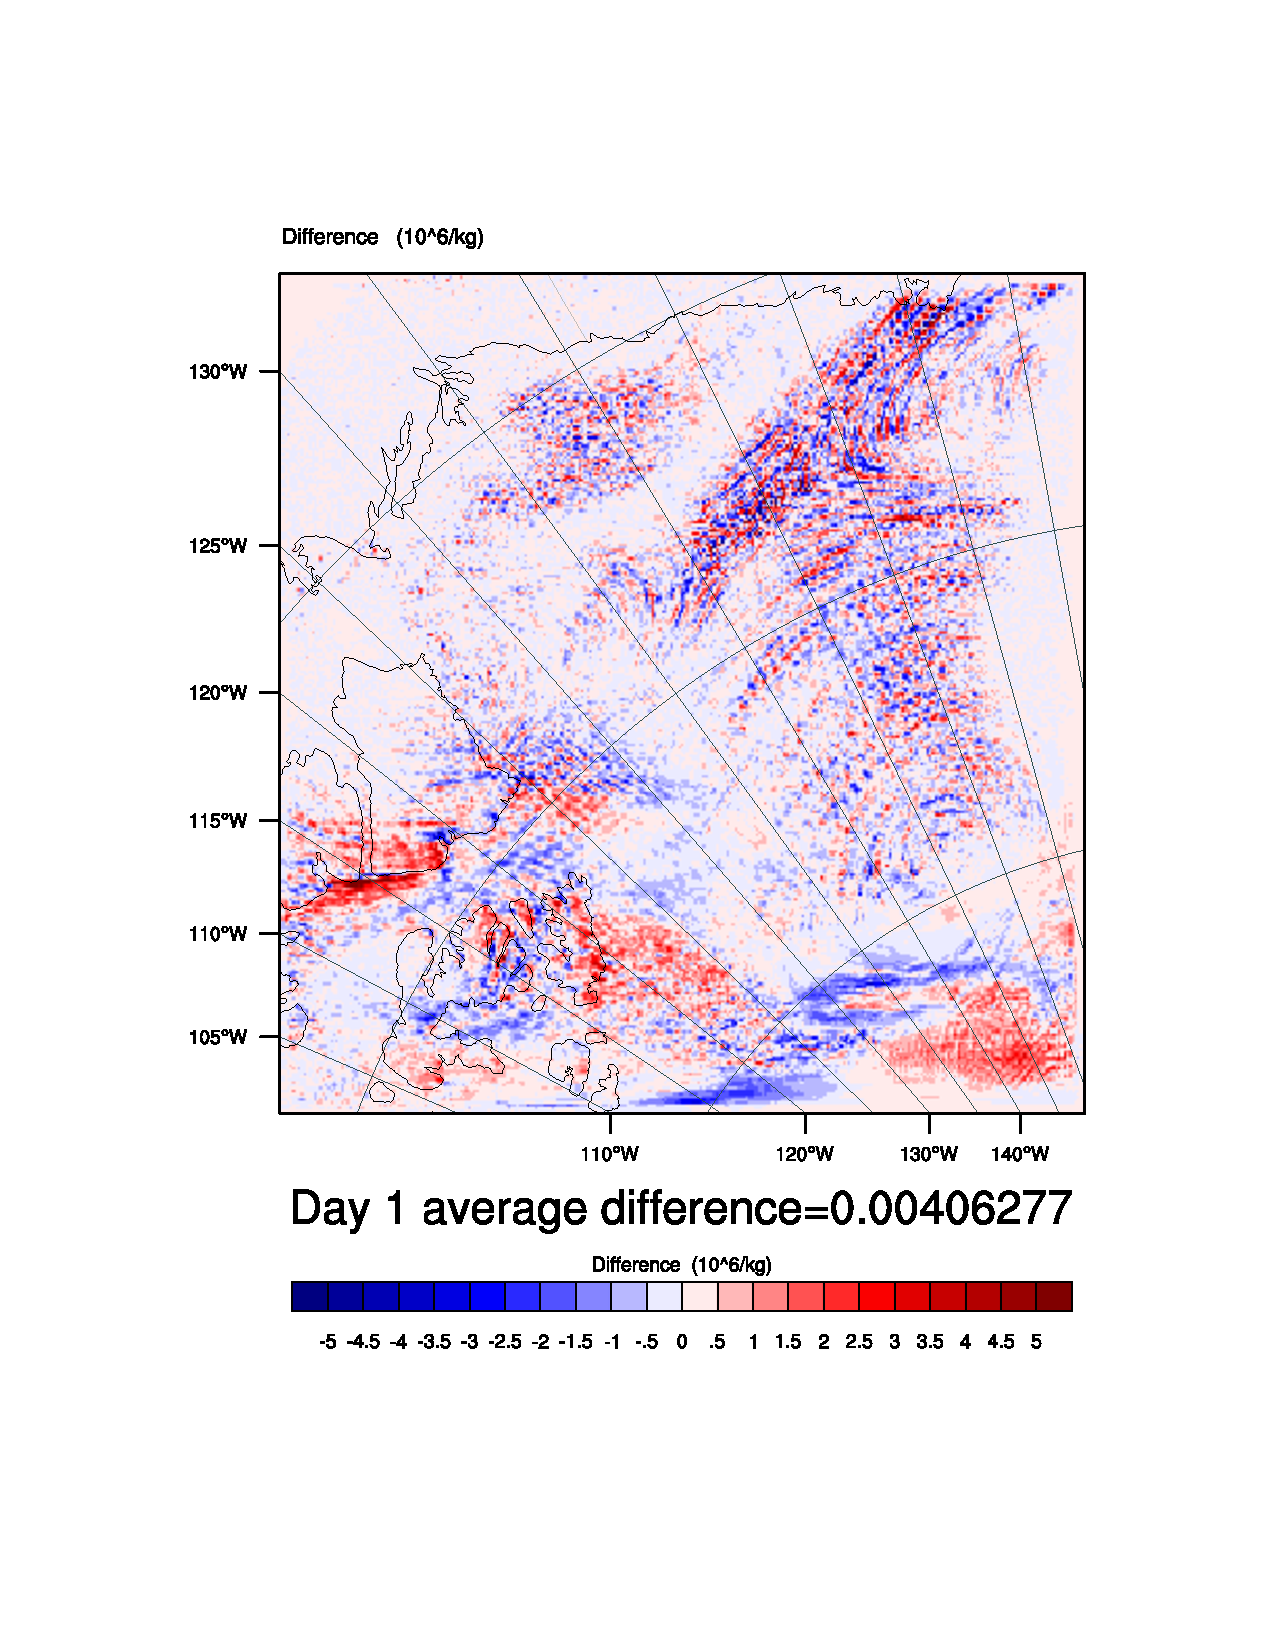
\includegraphics[width=\textwidth]{results/noice/diff_NoIce_QNCLOUD_Day1.pdf}
		\caption{CDNC, NoIce, day 1}
		\label{subfig:CDNCr2Day1}
	\end{subfigure}
	
	\begin{subfigure}{0.48\textwidth}
		\centering
		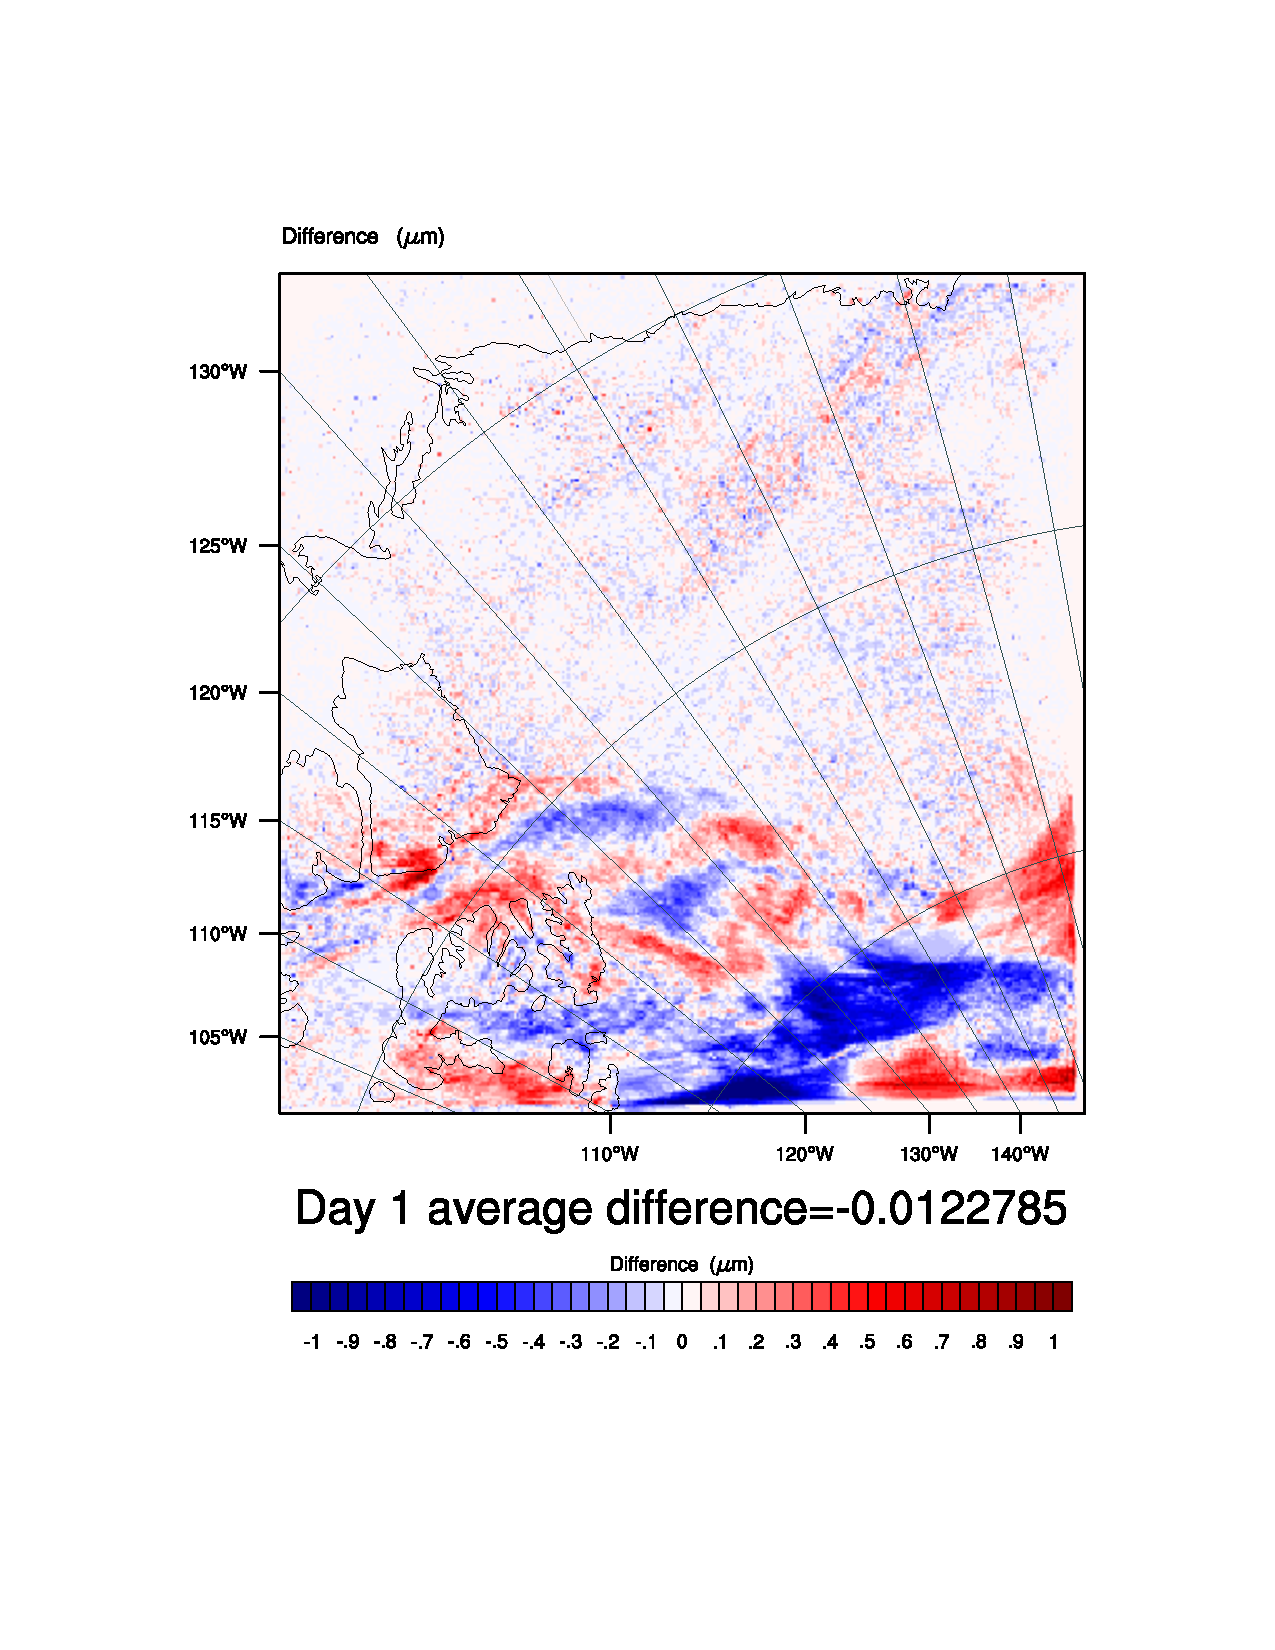
\includegraphics[width=\textwidth]{results/noice/diff_NoIce_RE_CLOUD_Day1.pdf}
		\caption{$r_e$, NoIce, day 1}
		\label{subfig:recloud_r2Day1}
	\end{subfigure}
\caption{Difference in time averaged LWP, and in height and time averaged CDNC and $r_e$, for day 1. NoIce-Control.}
\label{fig:lwpcdncre_r2Day1}
\end{figure}

Looking back to figure~\ref{subfig:LWPr1Day1}, there were no low in that area. This implies that there could be new clouds forming there, that could not form when there was sea ice. The removal of the sea ice has allowed for release of more aerosols (figure~\ref{subfig:aerocrossQNWFA}), increased evaporation and an increase in latent heat (LH) flux which can be seen from figure~\ref{subfig:lh_r2Day1}, where the shape of the area that sea ice was removed from is recognized. 

\begin{figure}
\centering
	\begin{subfigure}{0.48\textwidth}
		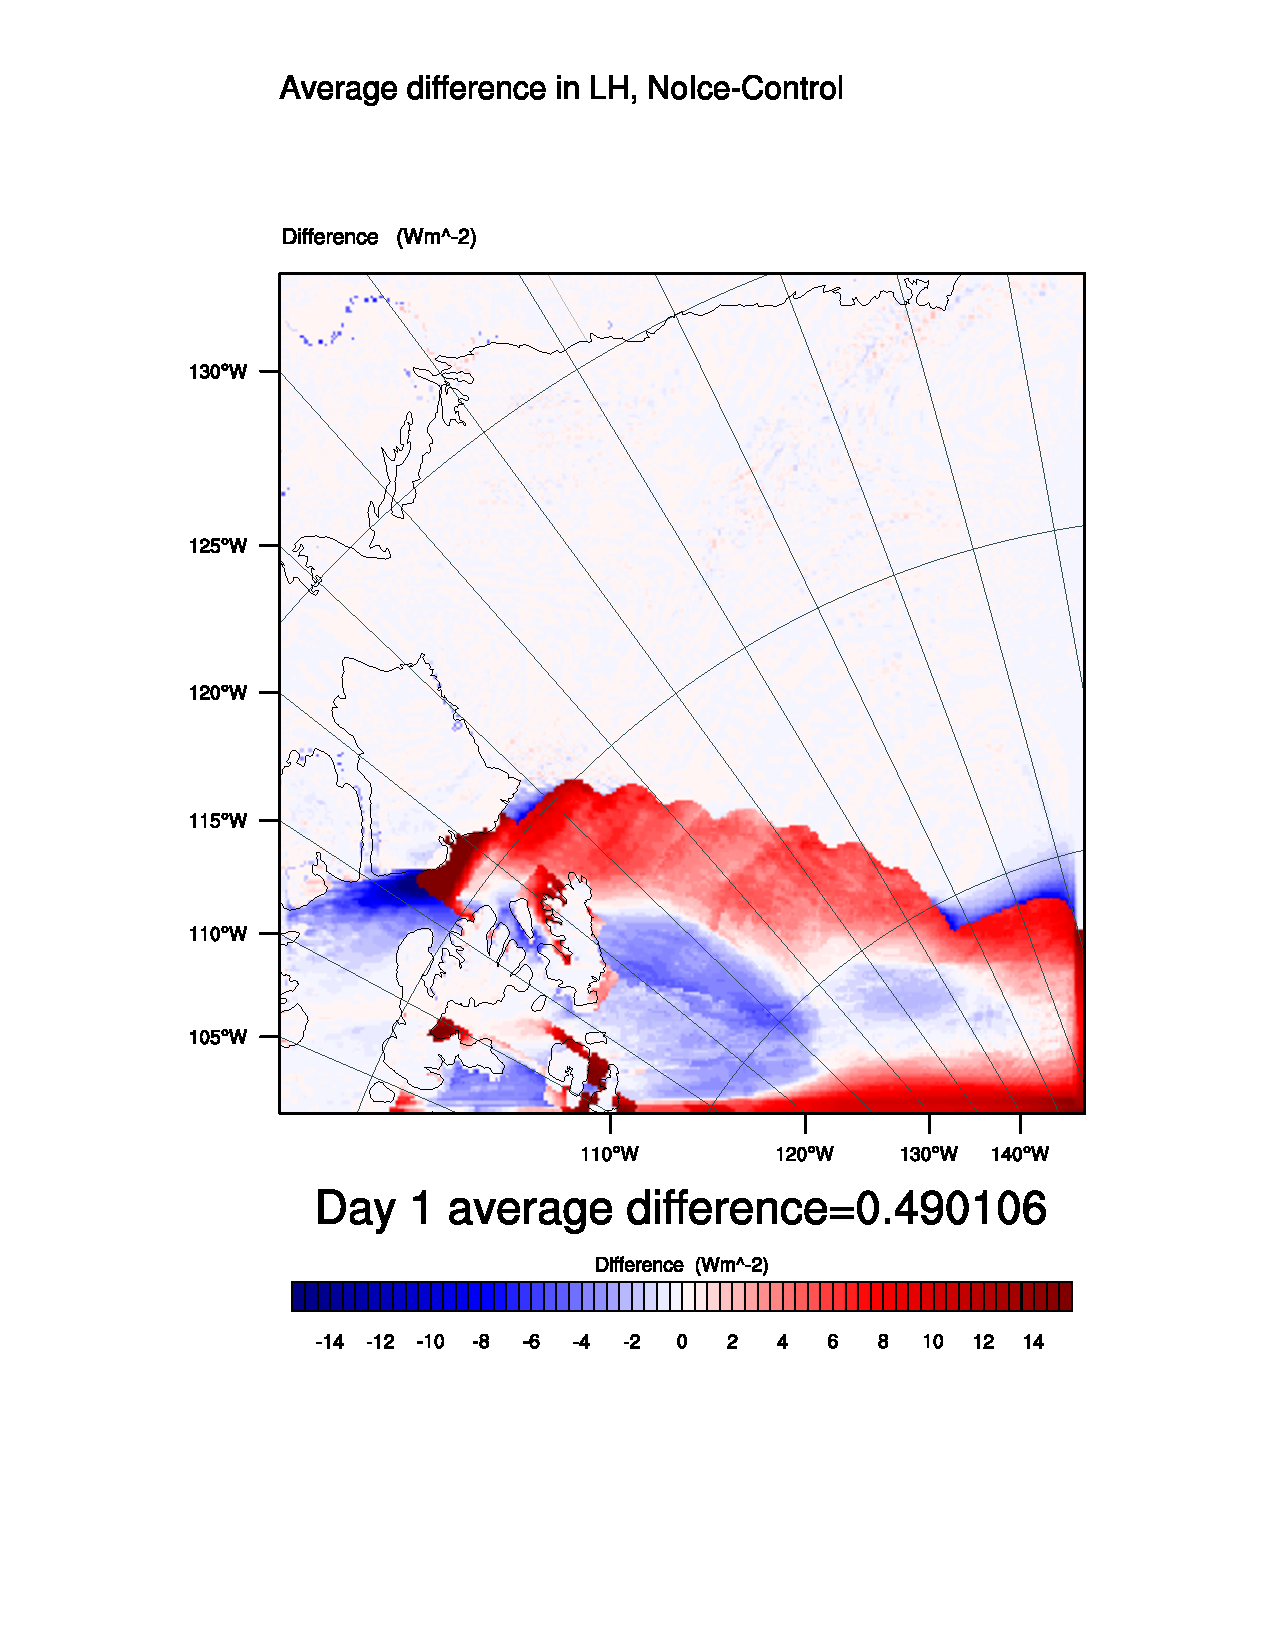
\includegraphics[width=\textwidth]{results/noice/diff_NoIce_LH_Day1.pdf}
		\caption{Difference in LH.}
		\label{subfig:lh_r2Day1}
	\end{subfigure}
	\quad
		\begin{subfigure}{0.48\textwidth}
		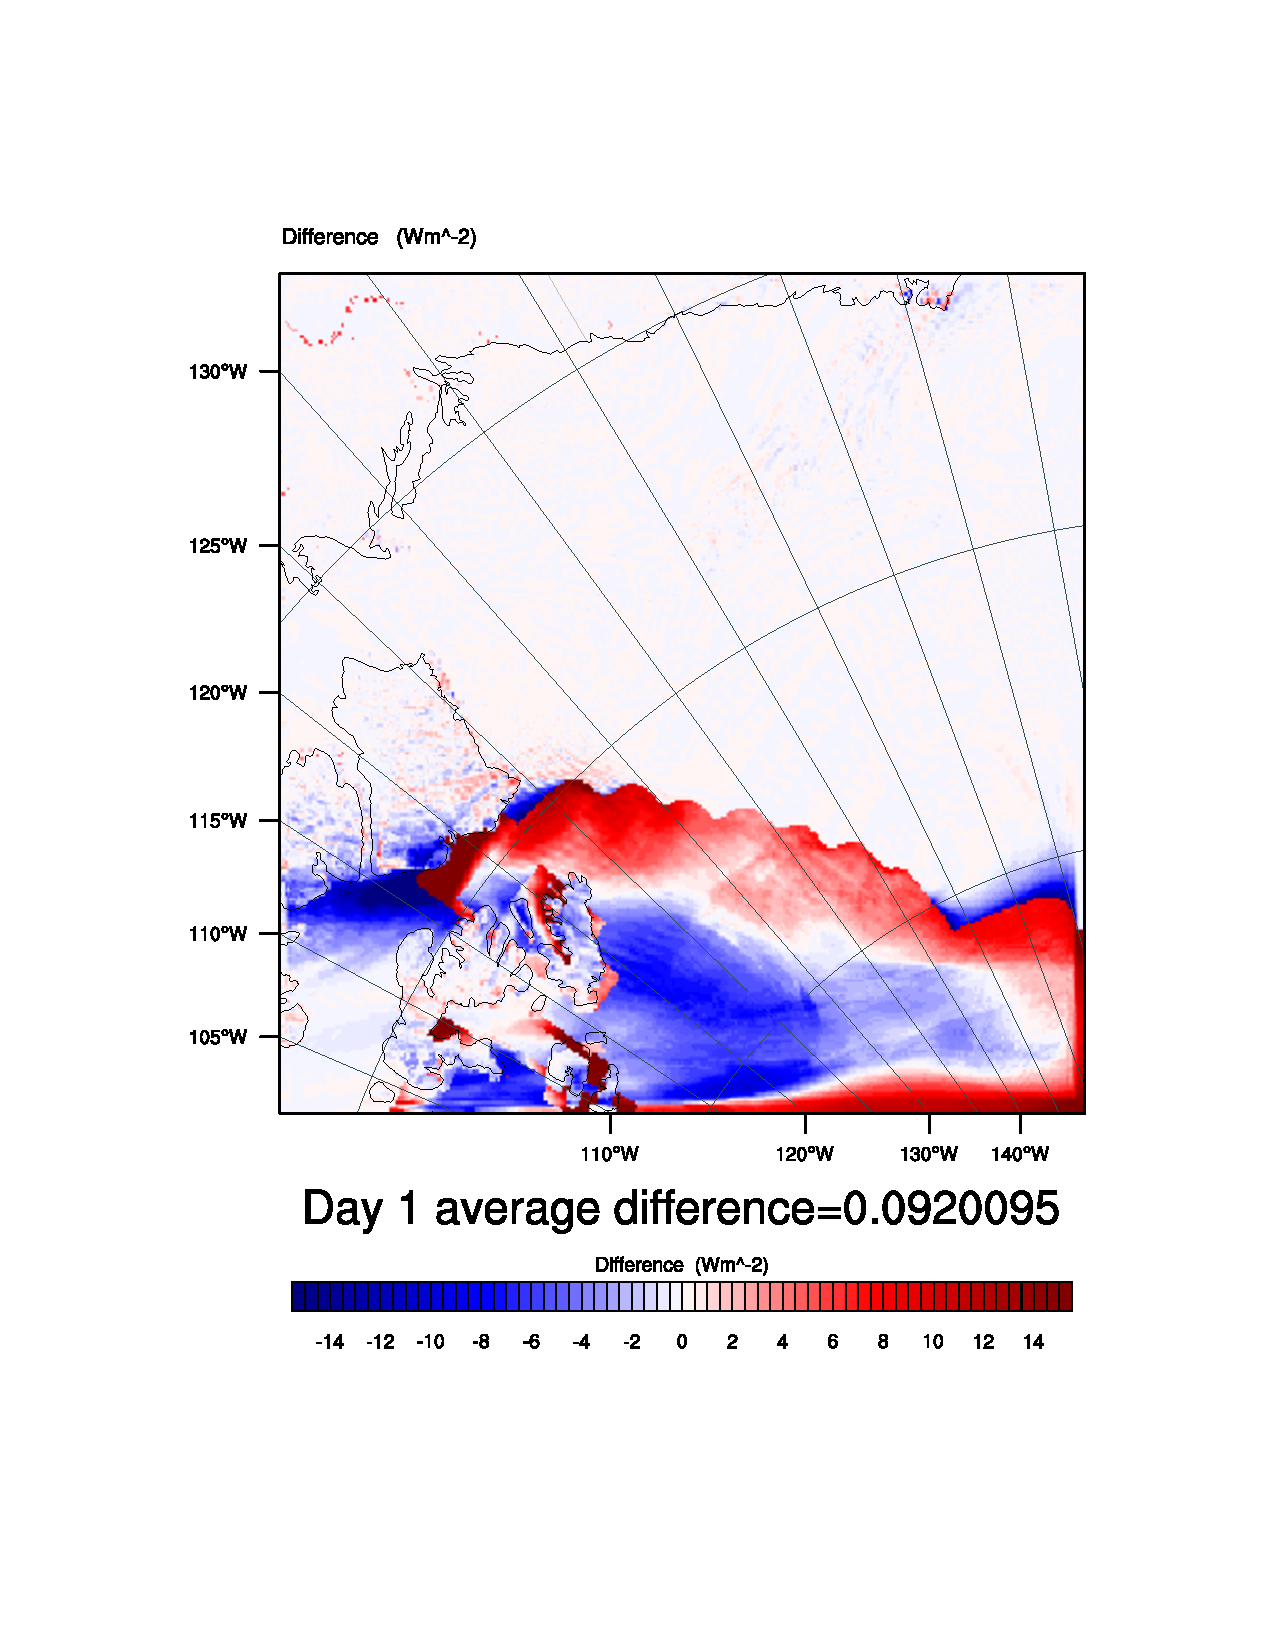
\includegraphics[width=\textwidth]{results/noice/diff_NoIce_HFX_Day1.pdf}
		\caption{Difference in SH.}
		\label{subfig:sh_r2Day1}
	\end{subfigure}
	
		\begin{subfigure}{0.48\textwidth}
		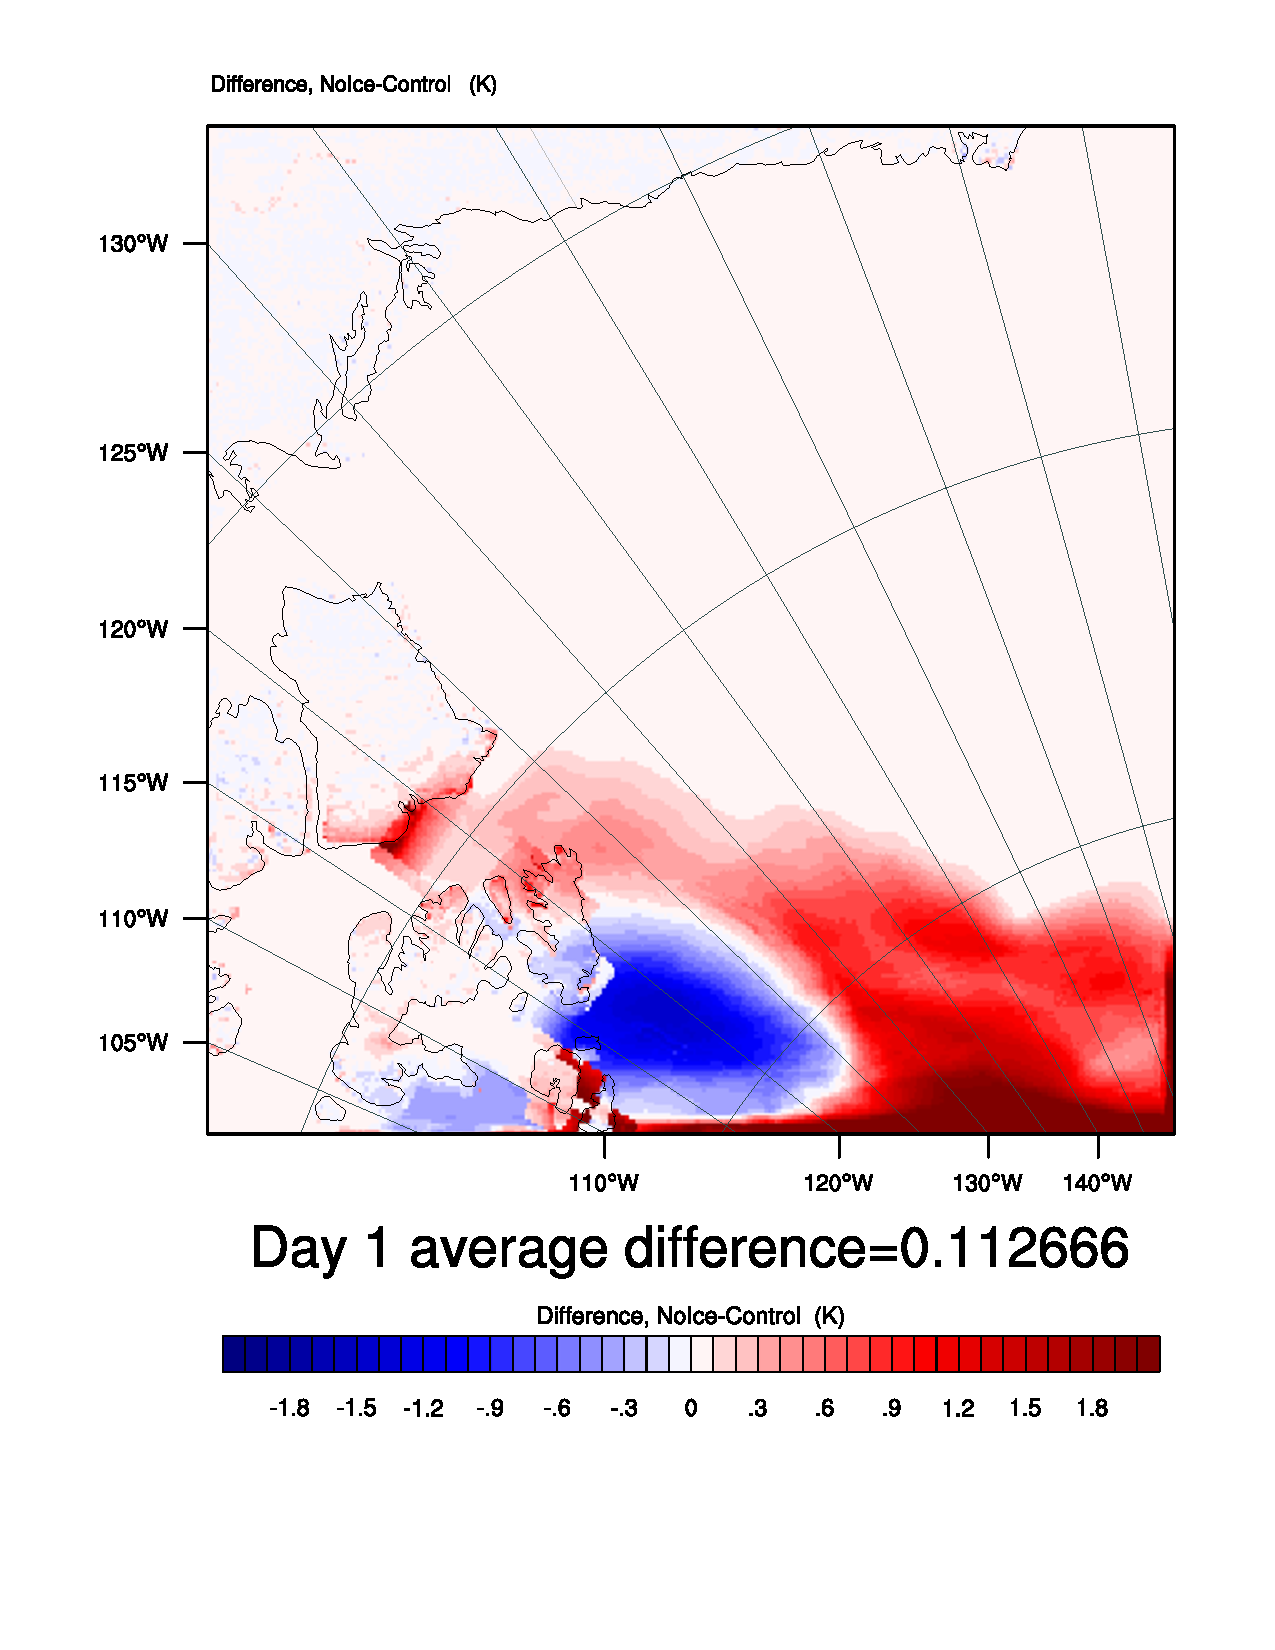
\includegraphics[width=\textwidth]{results/noice/diff_NoIce_skintemp_Day1.pdf}
		\caption{Difference in skin temperature.}
		\label{subfig:skin_r2Day1}
	\end{subfigure}
	\caption{Difference in time averaged LH, SH and skin temperature for day1. NoIce-Control.}
	\label{fig:lhshskin_r2Day1}
\end{figure}

The northernmost part of the study area also has an increase in the cloud droplet number concentration (CDNC), figure~\ref{subfig:CDNCr2Day1}, in the same area as is covered by the red patch indicating an increase in the LWP, which fits well with equation~\ref{eqn:LWC}. There the amount of liquid water is proportional to the droplet number concentration, denoted by $N$ in the equation, and the LWP is the vertically integrated LWC. The average increase in the CDNC would be approximately 1 or 2 droplets~$\text{cm}^{-3}$ in the northernmost area. Since CDNC is averaged over 24 hours and 11 layers (to a height of about 1800~m) the CDNC could be higher at certain times, and in certain layers.

The increase in effective radius in the same area as the LWP is increased also indicates the formation of new clouds,figure~\ref{subfig:recloud_r2Day1}, that could not form in the control run (see figure~\ref{subfig:recloud_r1Day1}).

In figure~\ref{subfig:recloud_r2Day1}, showing the difference in $r_e$, there are two red patches between 140 and 155$\degree$W at 80 and 83$\degree$N, indicating an increase in droplet effective radius. Looking back to figures~\ref{subfig:LWPr1Day1} and~\ref{subfig:recloud_r1Day1} of the LWP and $r_e$ from day 1 in the control run, there were no low clouds at those locations. The increase in LWP at 83$\degree$N has already been mentioned, but there is also a slight increase in LWP at 80$\degree$N where the other pronounced difference in $r_e$ is seen. These red patches of increased $r_e$ are also clear in the difference in LW downward radiation at the ground surface, figure~\ref{subfig:glw_r2Day1}. They can also be slightly recognized as a decrease in SW downward radiation in figure~\ref{subfig:swdown_r2Day1}. The SW radiation flux at ground surface has been reduced due to the increase in LWP, and the more pronounced decrease in downward SW is clearly recognized with the same shape and size as the northern patch of increase in LWP. This can be explained by equations~\ref{eqn:cloudalbedo} and~\ref{eqn:cloudtau}, where it is clear from equation~\ref{eqn:cloudtau} that the cloud optical depth, $\tau$, increases with LWP, and following equation~\ref{eqn:cloudalbedo} an increase in $\tau$ would also increase the cloud albedo.

\begin{figure}
\centering
	\begin{subfigure}{0.48\textwidth}
		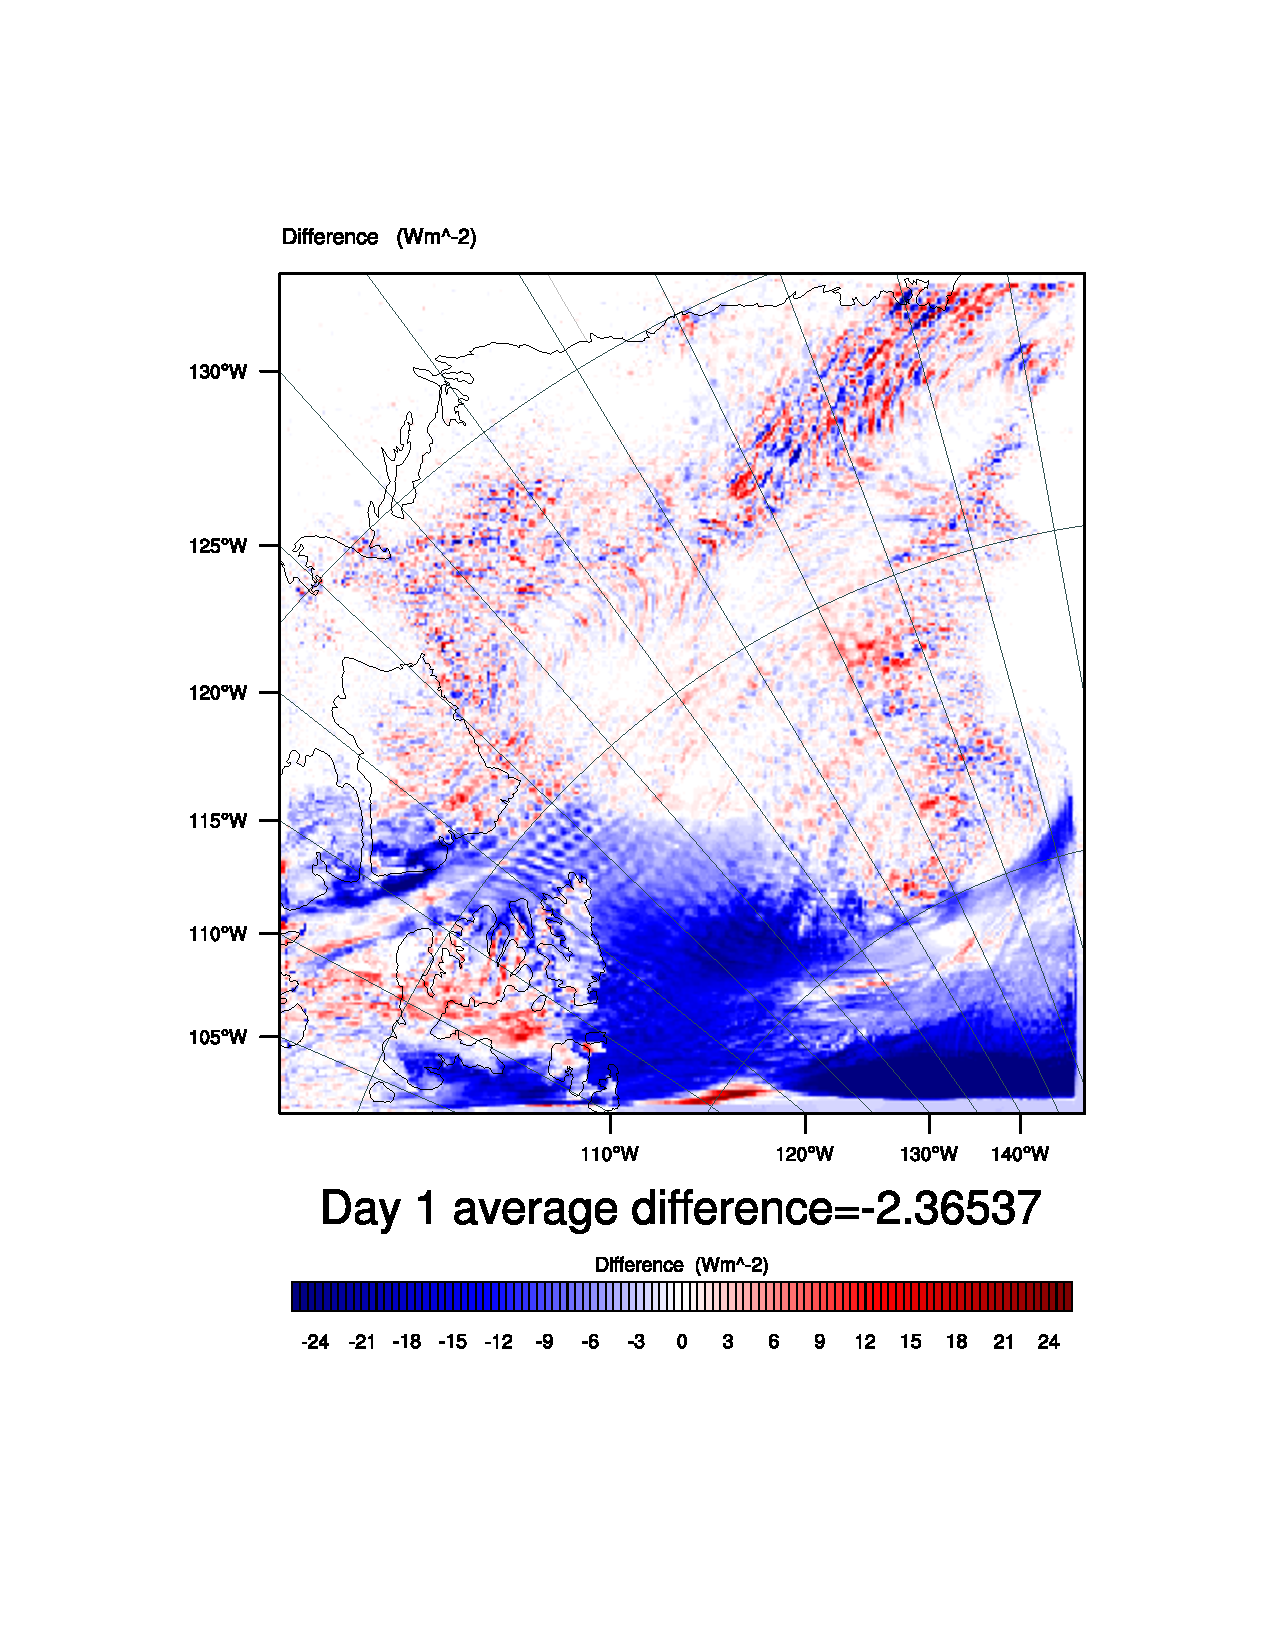
\includegraphics[width=\textwidth]{results/noice/diff_NoIce_SWDOWN_Day1.pdf}
		\caption{The average difference in SW flux down at the surface, day 1.}
		\label{subfig:swdown_r2Day1}
	\end{subfigure}
	\quad
	\begin{subfigure}{0.48\textwidth}
		\centering
		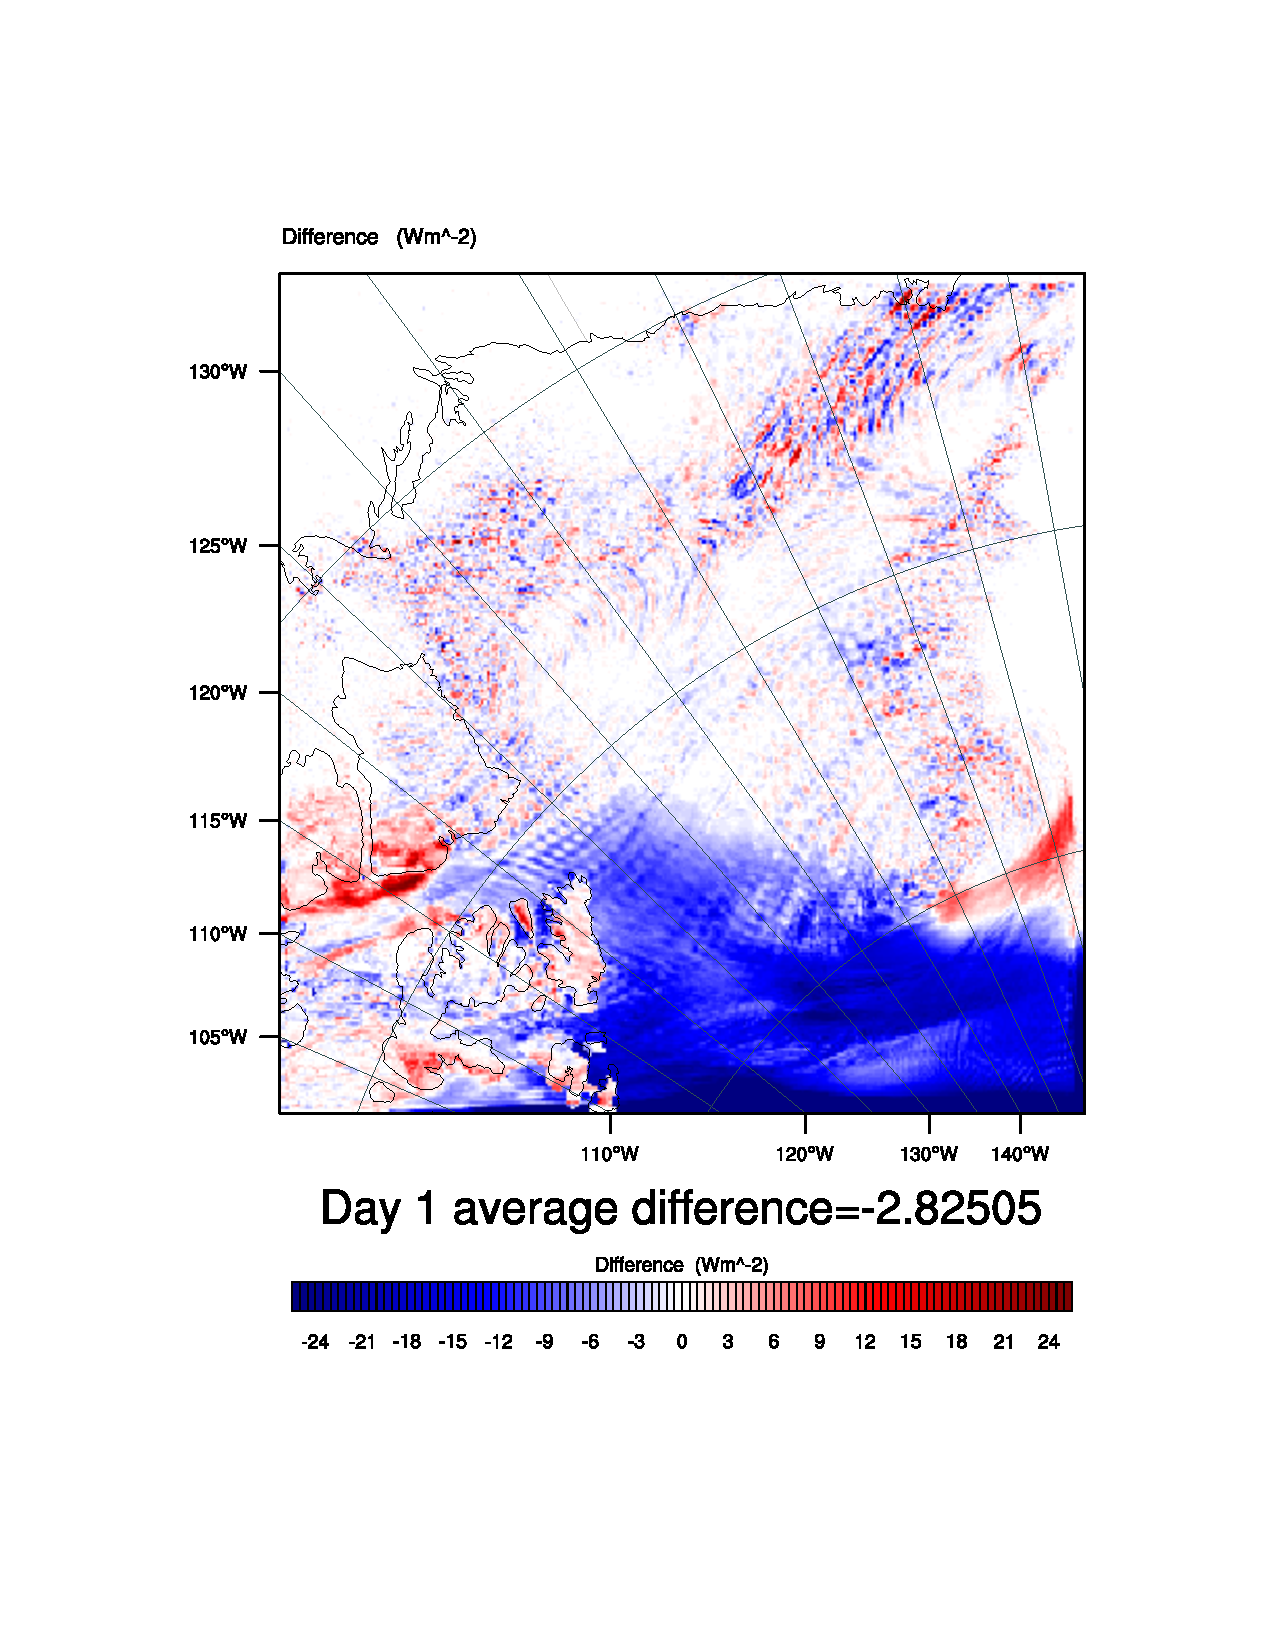
\includegraphics[width=\textwidth]{results/noice/diff_NoIce_SWUPT_Day1.pdf}
		\caption{The average difference in SW flux up at TOA, day 1.}
		\label{subfig:swup_r2Day1}
	\end{subfigure}
	
	\begin{subfigure}{0.48\textwidth}
		\centering
		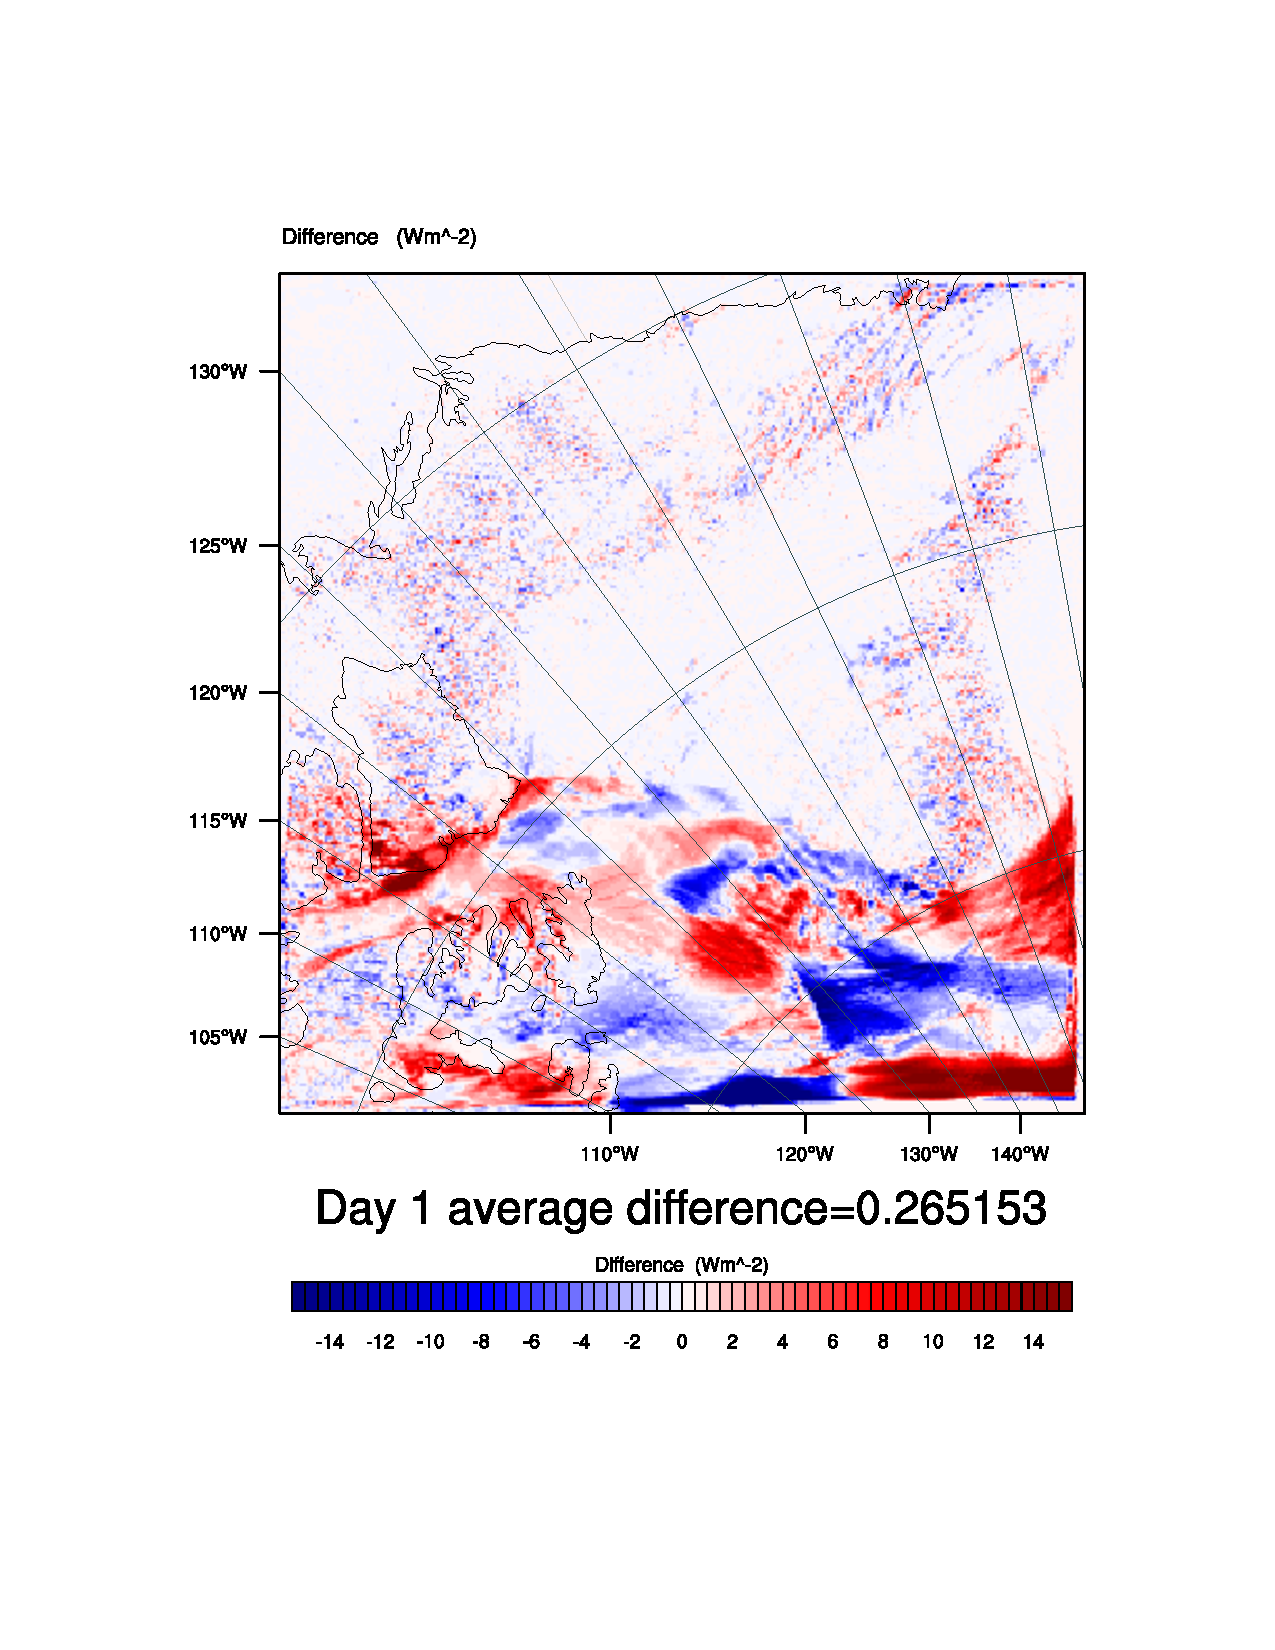
\includegraphics[width=\textwidth]{results/noice/diff_NoIce_GLW_Day1.pdf}
		\caption{The average difference in LW flux down at the surface, day 1.}
		\label{subfig:glw_r2Day1}
	\end{subfigure}
	\quad
	\begin{subfigure}{0.48\textwidth}
		\centering
		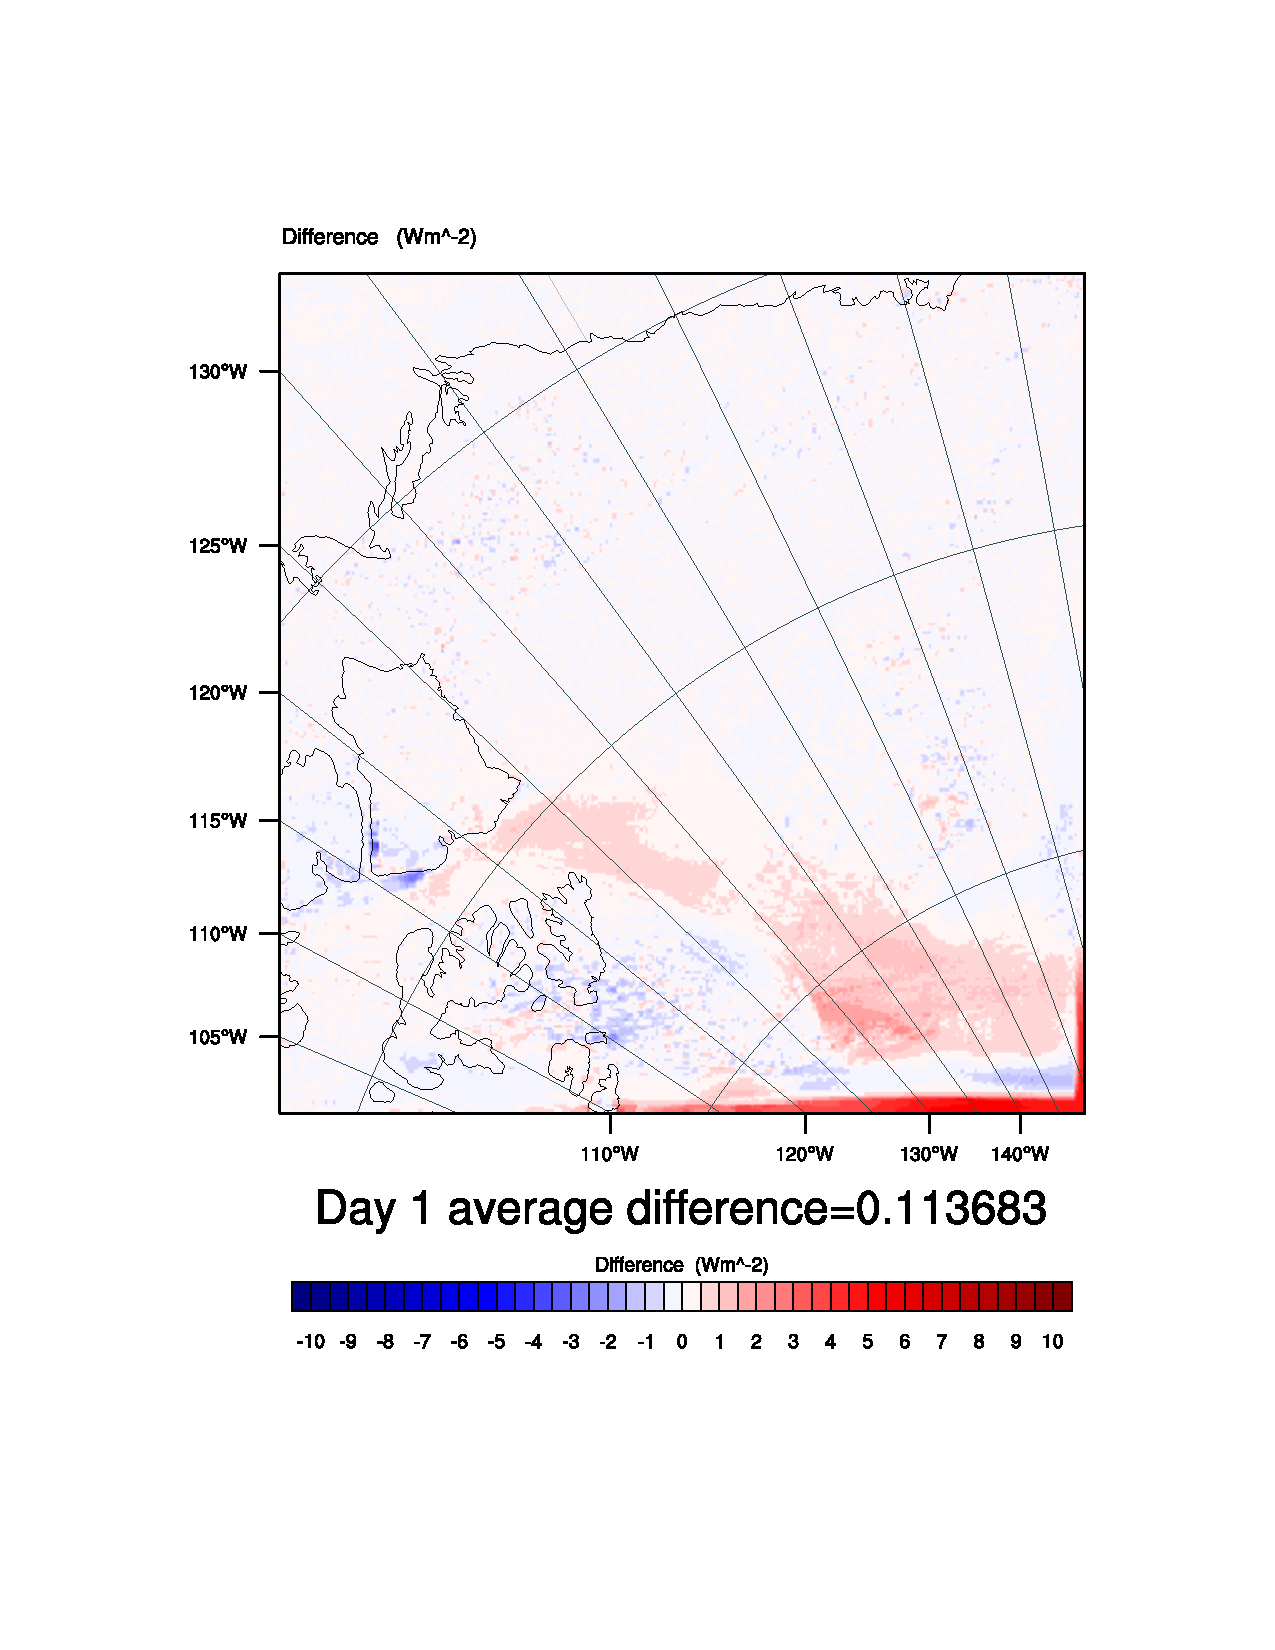
\includegraphics[width=\textwidth]{results/noice/diff_NoIce_LWUPT_Day1.pdf}
		\caption{The average difference in LW flux up at TOA, day 1.}
		\label{subfig:lwup_r2Day1}
	\end{subfigure}
	\caption{Difference in time averaged SW and LW flux down at the surface and up at TOA, for day 1. NoIce-Control.\\Notice the different scales.}
	\label{fig:radiation_r2Day1}
\end{figure}

The downward LW radiation flux at the surface (figure~\ref{subfig:glw_r2Day1}) has been increased due to the increase in LWP and droplet size, which means that there is more water in the clouds and they emit more LW to the ground. It was shown in Chapter~\ref{chap:theory} that an increase in LWP increases the emissivity of the cloud, shown in equation~\ref{eqn:epsilon_lw}, until the cloud is saturated with respect to LW radiation at about 40-45~$\text{g/m}^2$, following figure~\ref{fig:epsalb}. Similarly, but opposite sign, the decrease in LW down at the surface, at 81$\degree$N 125-140$\degree$W, is recognized as a decrease also in LWP, CDNC and $r_e$ (figures~\ref{subfig:LWPr2Day1},~\ref{subfig:CDNCr2Day1} and~\ref{subfig:recloud_r2Day1}). Thus there are less, or at least thinner, clouds in that area to emit LW. The decrease in LWP by $\sim$9~$\text{g/m}^2$ (figure~\ref{subfig:LWPr2Day1}) from $\sim$40~$\text{g/m}^2$ in the control run (figure~\ref{subfig:LWPr1Day1}) significantly decreases the cloud emissivity since it does not vary linearly and is below 40~$\text{g/m}^2$ (recall figure~\ref{fig:epsalb}). The increase in the LW at TOA (figure~\ref{subfig:lwup_r2Day1}) is because of increased temperature at the surface when the sea ice is removed (figure~\ref{subfig:skin_r2Day1}).

Of course, the removal of sea ice would reduce the SW at TOA, see figure~\ref{subfig:swup_r2Day1}. The albedo of sea ice varies between 0.5 and 0.9 depending on snow cover and the age of the ice and is typically 0.5-0.7 for bare ice, whereas a typical ocean albedo is 0.06~\citep{NSIDC}. Thus the change in SW at TOA is negative over the area of ocean where there was sea ice in the control run. The increased SW at TOA at 80$\degree$N and 155$\degree$W is because of the cloud forming in that area, see figure~\ref{subfig:swup_r2Day1}, and can be recognized in the increase in $r_e$ in the same place (figure~\ref{subfig:recloud_r2Day1}). This also gives an increase in LWP (figure~\ref{subfig:LWPr2Day1}) and reduction in SW at surface (figure~\ref{subfig:swdown_r2Day1}) and increase of LW at surface (figure~\ref{subfig:glw_r2Day1}). The signal in upward SW at TOA is due to the enhanced albedo caused by new clouds at that location, since these figures don't show in-cloud changes, simply the difference between the fields from the run without ice (NoIce) and the control run (Control).

A part of the decrease in SW down at the surface (figure~\ref{subfig:swdown_r2Day1}) has the same shape as that of decreased SW up at TOA (figure~\ref{subfig:swup_r2Day1}), especially around 75-80$\degree$N 110-135$\degree$W. The removal of sea ice has not just decreased the SW up at TOA by decreasing the albedo, but also the downward SW at the surface is decreased. Of the SW reflected by the sea ice, a fraction (depending on the clouds albedo) would be reflected back to the sea ice by the overlying lower clouds. This effect is lost when the sea ice is removed. Even though there is $\sim$2.4~$\text{W/m}^2$ less SW down at the surface, the SW that does reach the surface will have a warming effect compared to the control run, since the ocean has such a low albedo (0.06).

The heat fluxes and surface temperature are almost unchanged for most of the study area by the removal of sea ice, except for the area where the sea ice has been removed (see figures~\ref{subfig:lh_r2Day1},~\ref{subfig:sh_r2Day1} and~\ref{subfig:skin_r2Day1}). For much of the "sea ice removed area" the fluxes are higher than in the control run. This is not surprising, since one would expect the ocean surface to hold a higher temperature than the sea ice, therefore more heat is released than in the case when sea ice is present. This is true except for the blue area at 77-79$\degree$N and 115-125$\degree$W, also from which sea ice has been removed. This indicates a decrease in surface heat fluxes and surface temperature compared with the control run. This area of decrease in each of the figures, coincides with where the heat fluxes were higher than over the rest of the sea ice by $\sim$5 to 10~$\text{W/m}^2$ in the control run, see figures~\ref{subfig:lh_r1Day1} and~\ref{subfig:sh_r1Day1}, and where the skin temperature was higher, see figure~\ref{subfig:skin_r1Day1}. Thus the surface heat fluxes are approximately the same for the whole area which is now sea ice free, but had to increase and decrease in different areas. The same goes for the temperature, which was $\sim$2$\degree$C higher in that area than the rest of the sea ice, in the control run. Now the surface is colder in there, about 0.9 to 1.5$\degree$C colder. The open ocean around has a temperature which is $\sim$1$\degree$C warmer, thus evening out the difference in temperature between that and the area of decrease, leaving the whole "sea ice removed area" with approximately the same temperature. The average increase in skin temperature for the whole area is 0.1$\degree$C.

%----------------
\clearpage
\subsection{Day 5}
%----------------
The average differences for LWP, CDNC and $r_e$ at day 5 are all negative, see figure~\ref{fig:lwpcdncre_r2Day5}, over the area that had ice in the control run. Thus the clouds making up the LWP in the control run, see figure~\ref{subfig:LWPr1Day5}, have either ceased to exist, been significantly thinned, moved away or turned into ice. The LWP has a negative difference of >15~$\text{g/m}^2$ for most of the "sea ice removed area", which means that the LWP, when comparing with the values for that area in the control run (figure~\ref{subfig:LWPr1Day5}) which were around 40-100~$\text{g/m}^2$, there is still around 20-70$\text{g/m}^2$ left. So the clouds have not all ceased to exist. This is supported by the fact that the CDNC in the control run was $\sim$10 to 25~$\text{cm}^{-3}$ and has according to figure~\ref{subfig:CDNCr2Day5} got 3 to >5 droplets~$\text{cm}^{-3}$ less in the run with no ice. Then the clouds in the run with no ice are left with <5 to around 20 droplets~$\text{cm}^{-3}$ which is definitely enough to assume that there are still clouds in the area.

\begin{figure}[hb]
\centering
	\begin{subfigure}{0.48\textwidth}
		\centering
		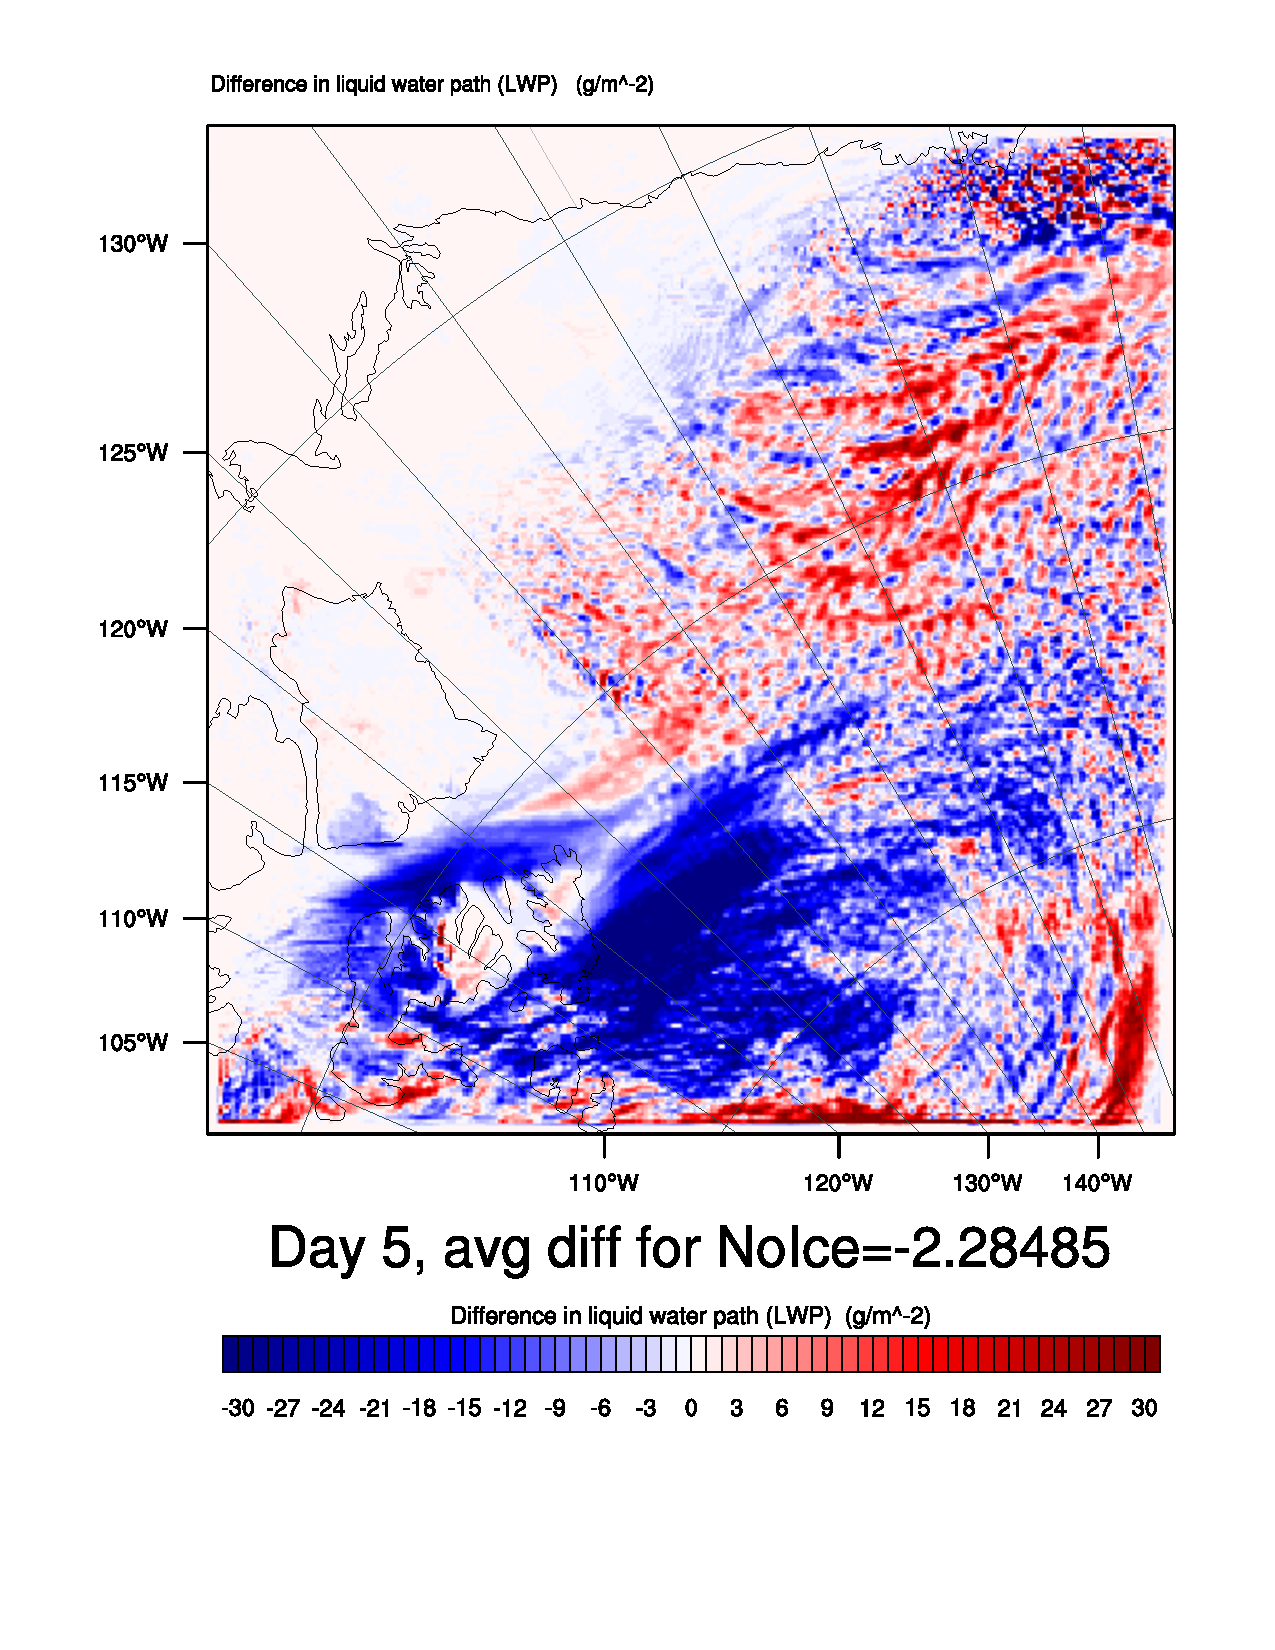
\includegraphics[width=\textwidth]{results/noice/Diff_LWP_Day5NoIce.pdf}
		\caption{LWP, NoIce, day 5}
		\label{subfig:LWPr2Day5}
	\end{subfigure}
	\quad
	\begin{subfigure}{0.48\textwidth}
		\centering
		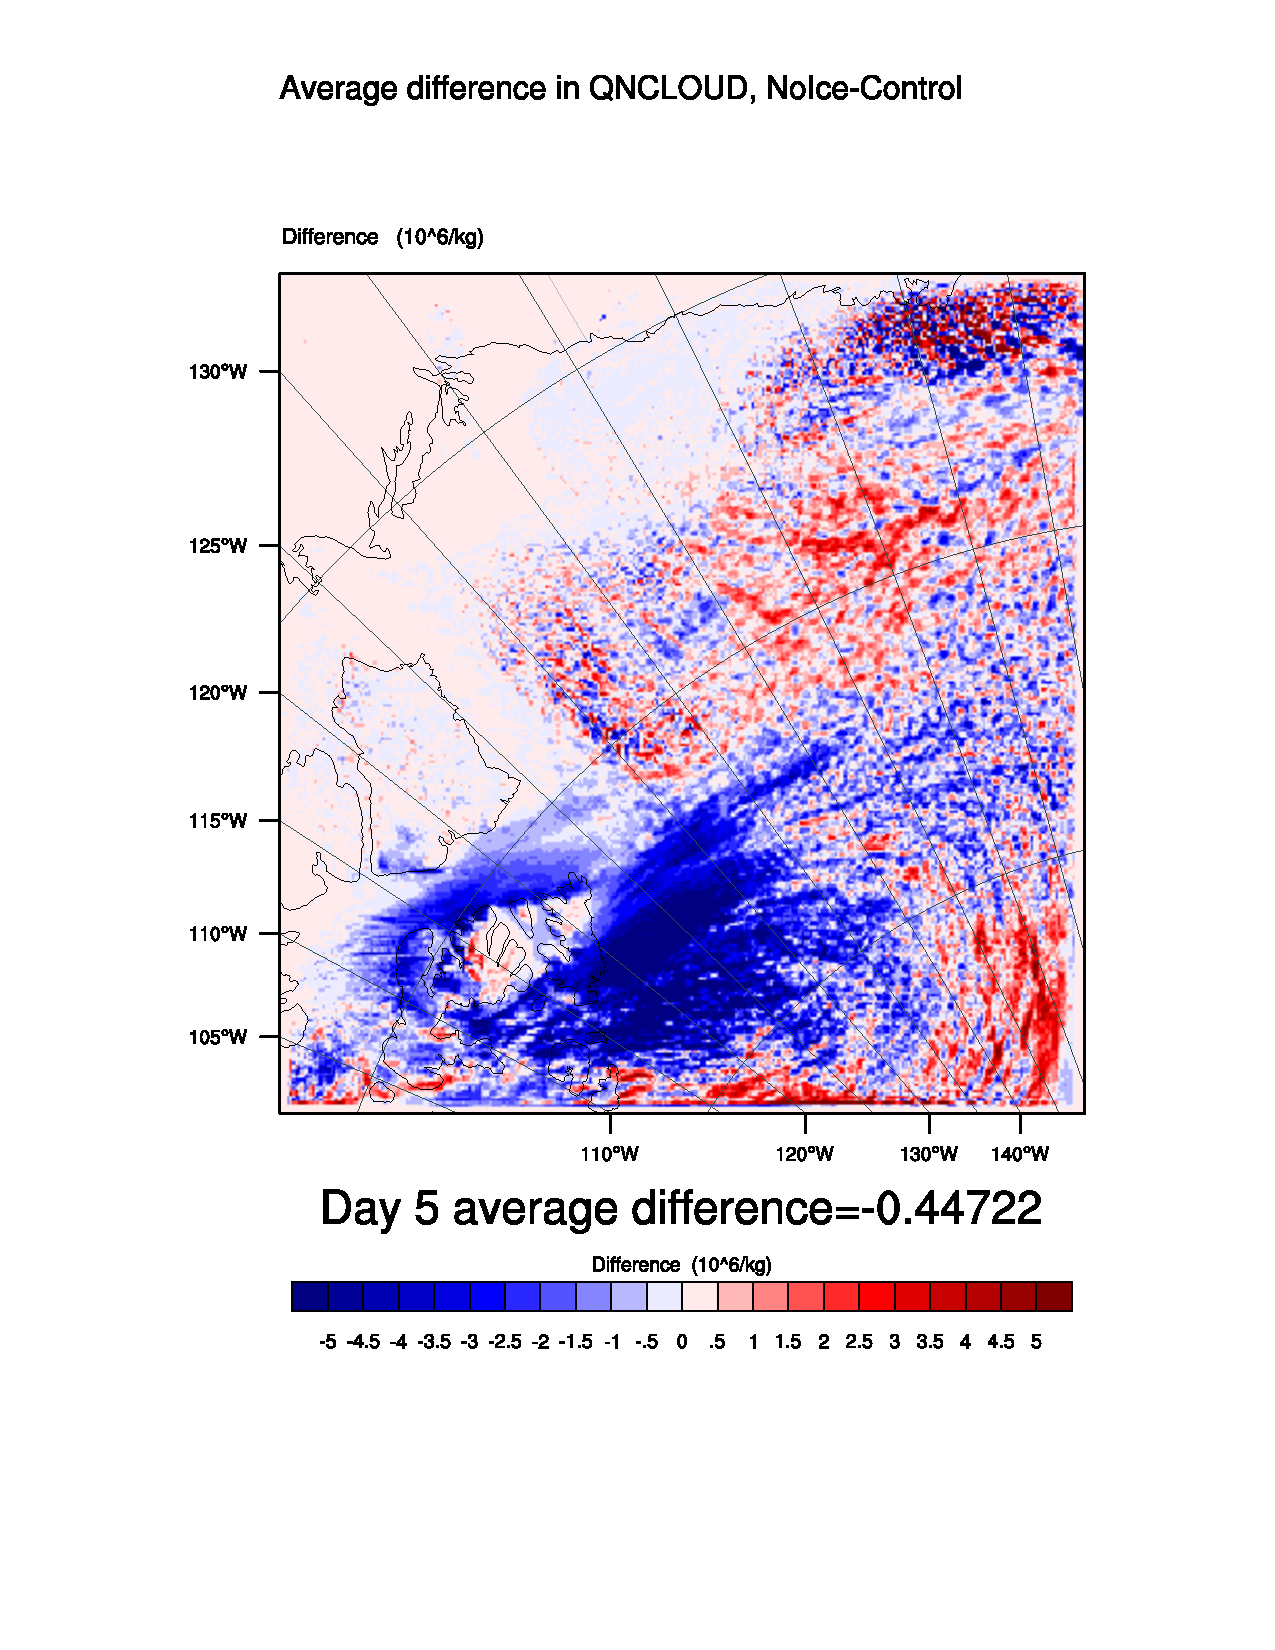
\includegraphics[width=\textwidth]{results/noice/diff_NoIce_QNCLOUD_Day5.pdf}
		\caption{CDNC, NoIce, day 5}
		\label{subfig:CDNCr2Day5}
	\end{subfigure}
	
	\begin{subfigure}{0.48\textwidth}
		\centering
		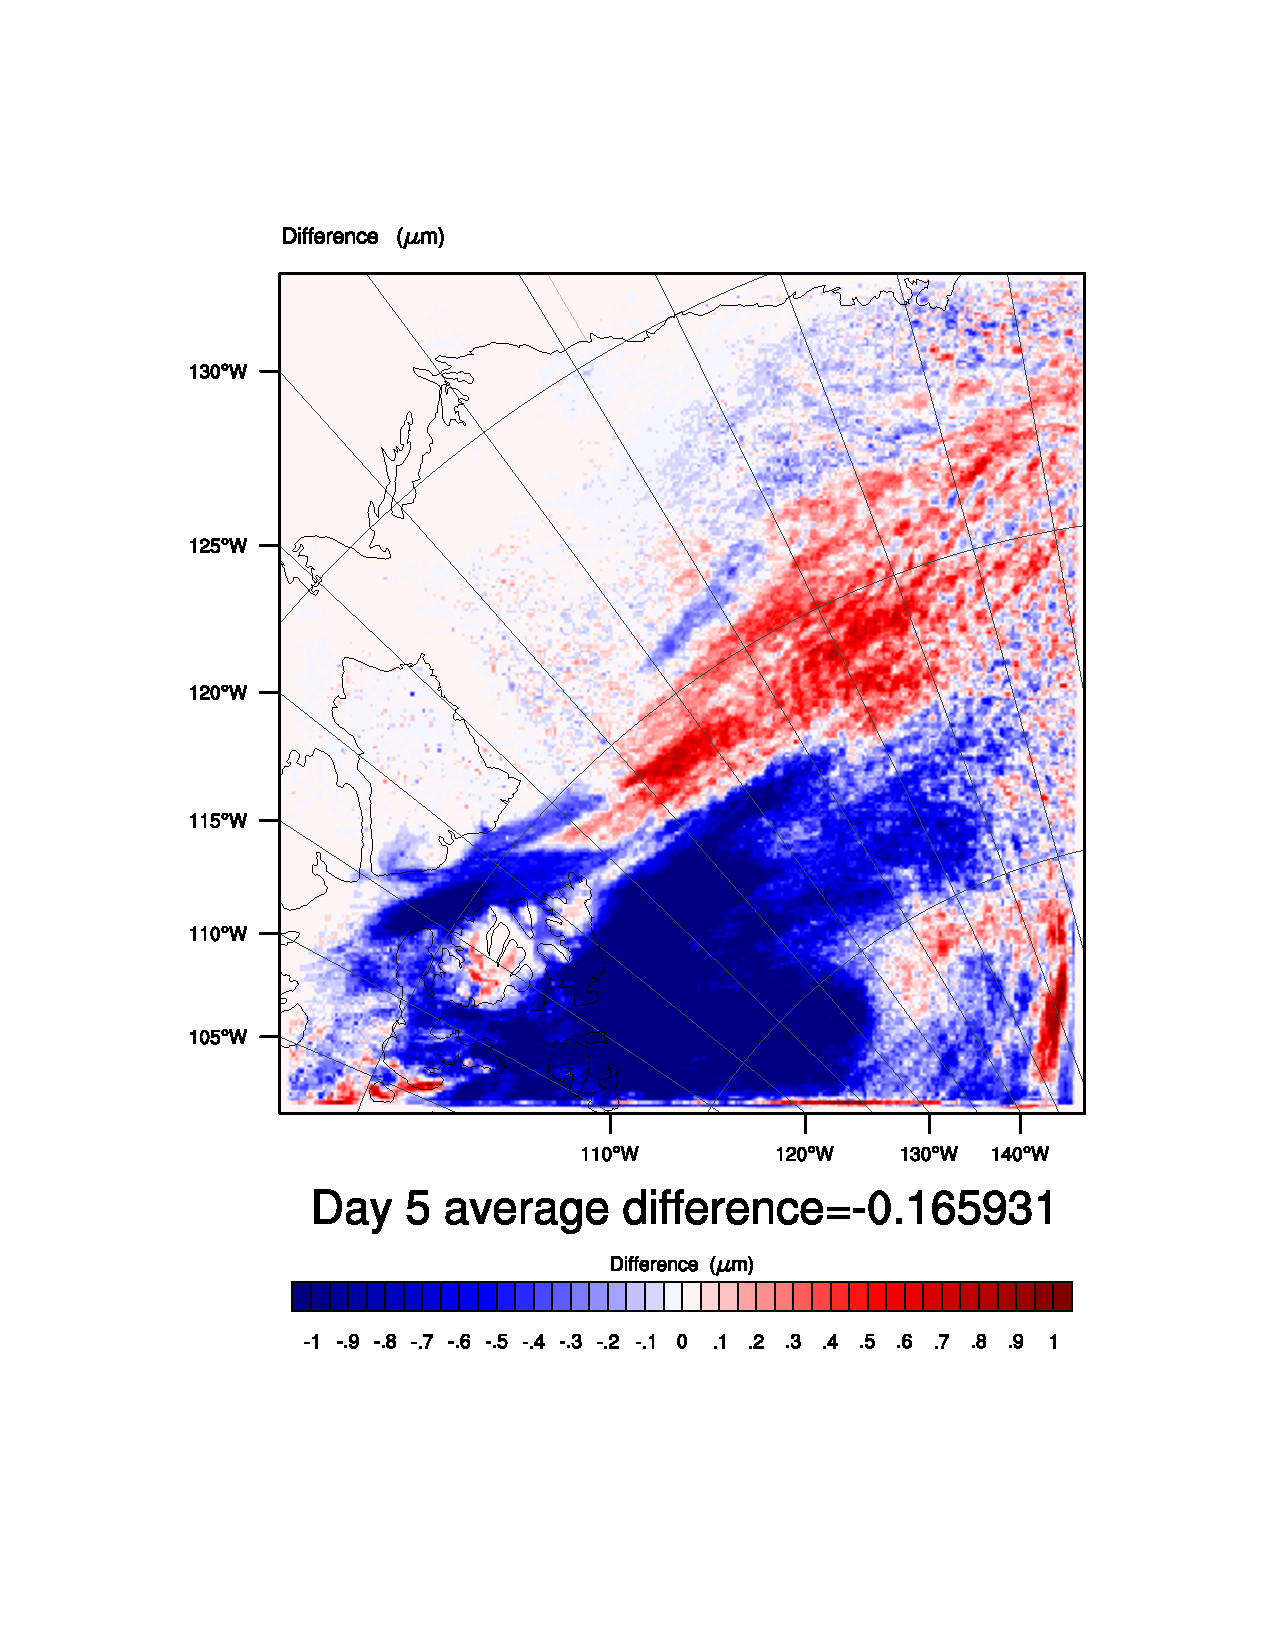
\includegraphics[width=\textwidth]{results/noice/diff_NoIce_RE_CLOUD_Day5.pdf}
		\caption{$r_e$, NoIce, day 5}
		\label{subfig:recloud_r2Day5}
	\end{subfigure}
\caption{Difference in time averaged LWP, and in height and time averaged CDNC and $r_e$, for day 5. NoIce-Control.}
\label{fig:lwpcdncre_r2Day5}
\end{figure}

There is hardly any ice at all in the study area in the lowermost 1800~m (not shown), and the IWP is zero (not shown) over the area where there was sea ice, and the area around. The wind pattern (not shown) is the same as in the control run (figure~\ref{subfig:weather_cont_day5}), and the chance that the clouds have been moved to a different area is ruled out. Therefore precipitation must have depleted the clouds of some of the droplets. The difference in rain (not shown) for the run with no ice compared to the control run is negligible and so snow was found guilty of depleting the clouds. Figure~\ref{fig:snowstory} shows how the clouds that were claimed started to form in day 1 of the run with no ice, in section~\ref{sec:noiceDay1}, did form and as more water vapor and aerosols were made available, more clouds developed and produced snow that performed natural cloud seeding, by making other clouds snow too.

\begin{figure}
\centering
	\begin{subfigure}{0.32\textwidth}
		\centering
		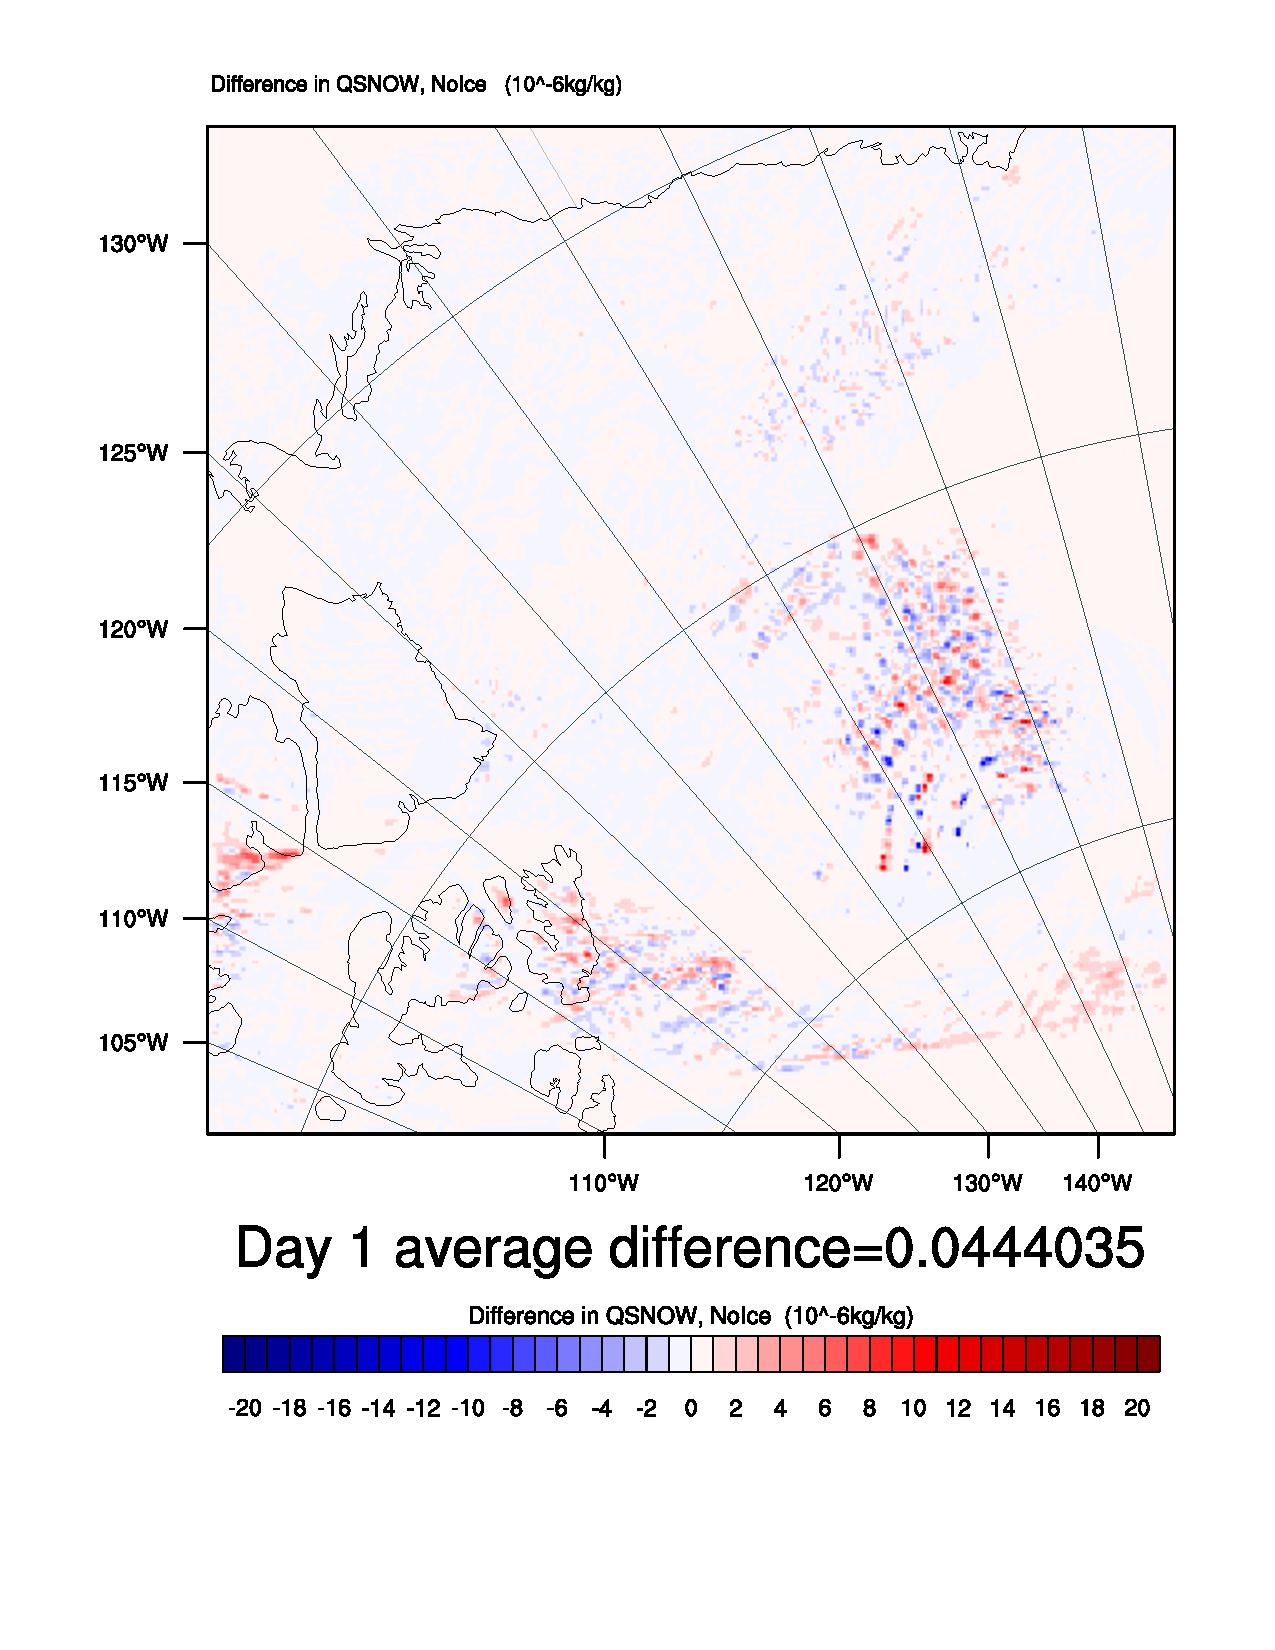
\includegraphics[width=\textwidth]{results/noice/diff_NoIce_qsnow_Day1.pdf}
		\caption{Day 1}
		\label{subfig:snowstory_Day1}
	\end{subfigure}
	\begin{subfigure}{0.32\textwidth}
		\centering
		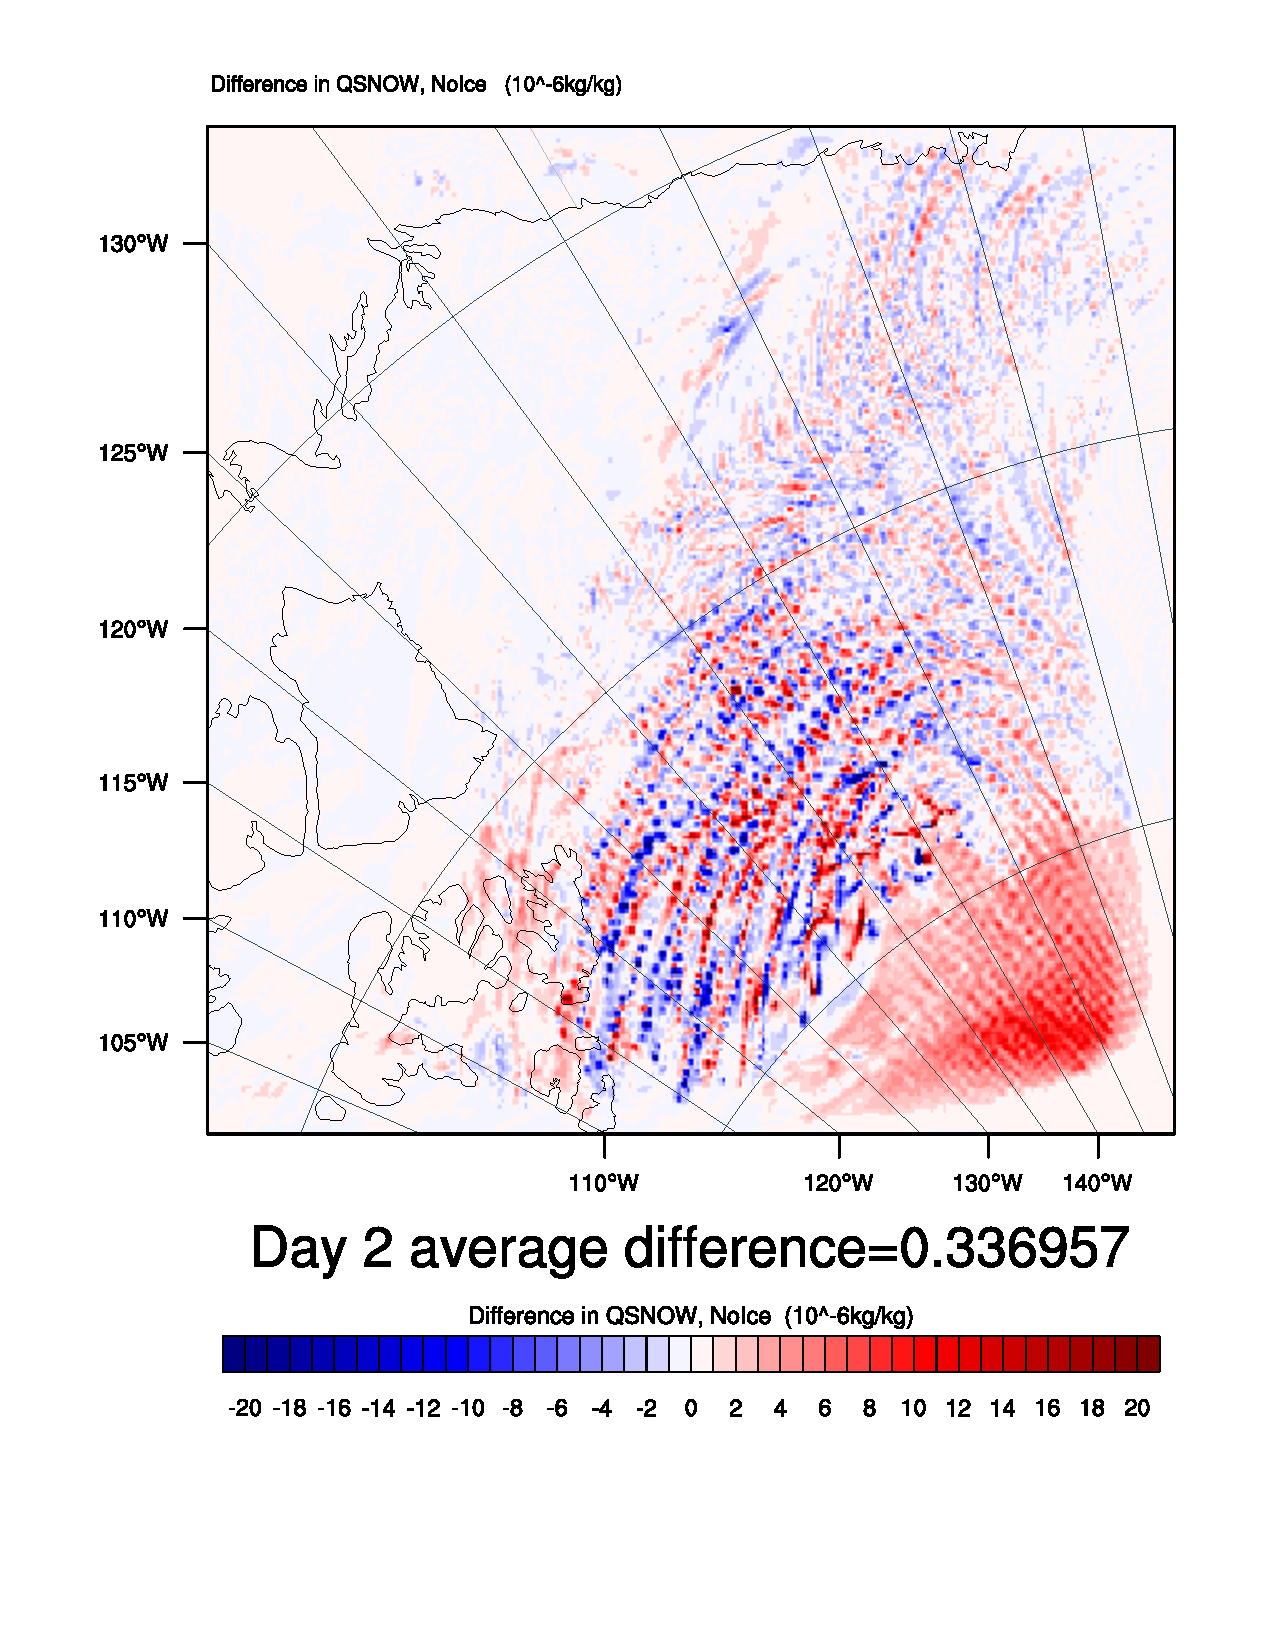
\includegraphics[width=\textwidth]{results/noice/diff_NoIce_qsnow_Day2.pdf}
		\caption{Day 2}
		\label{subfig:snowstory_Day2}
	\end{subfigure}
	\begin{subfigure}{0.32\textwidth}
		\centering
		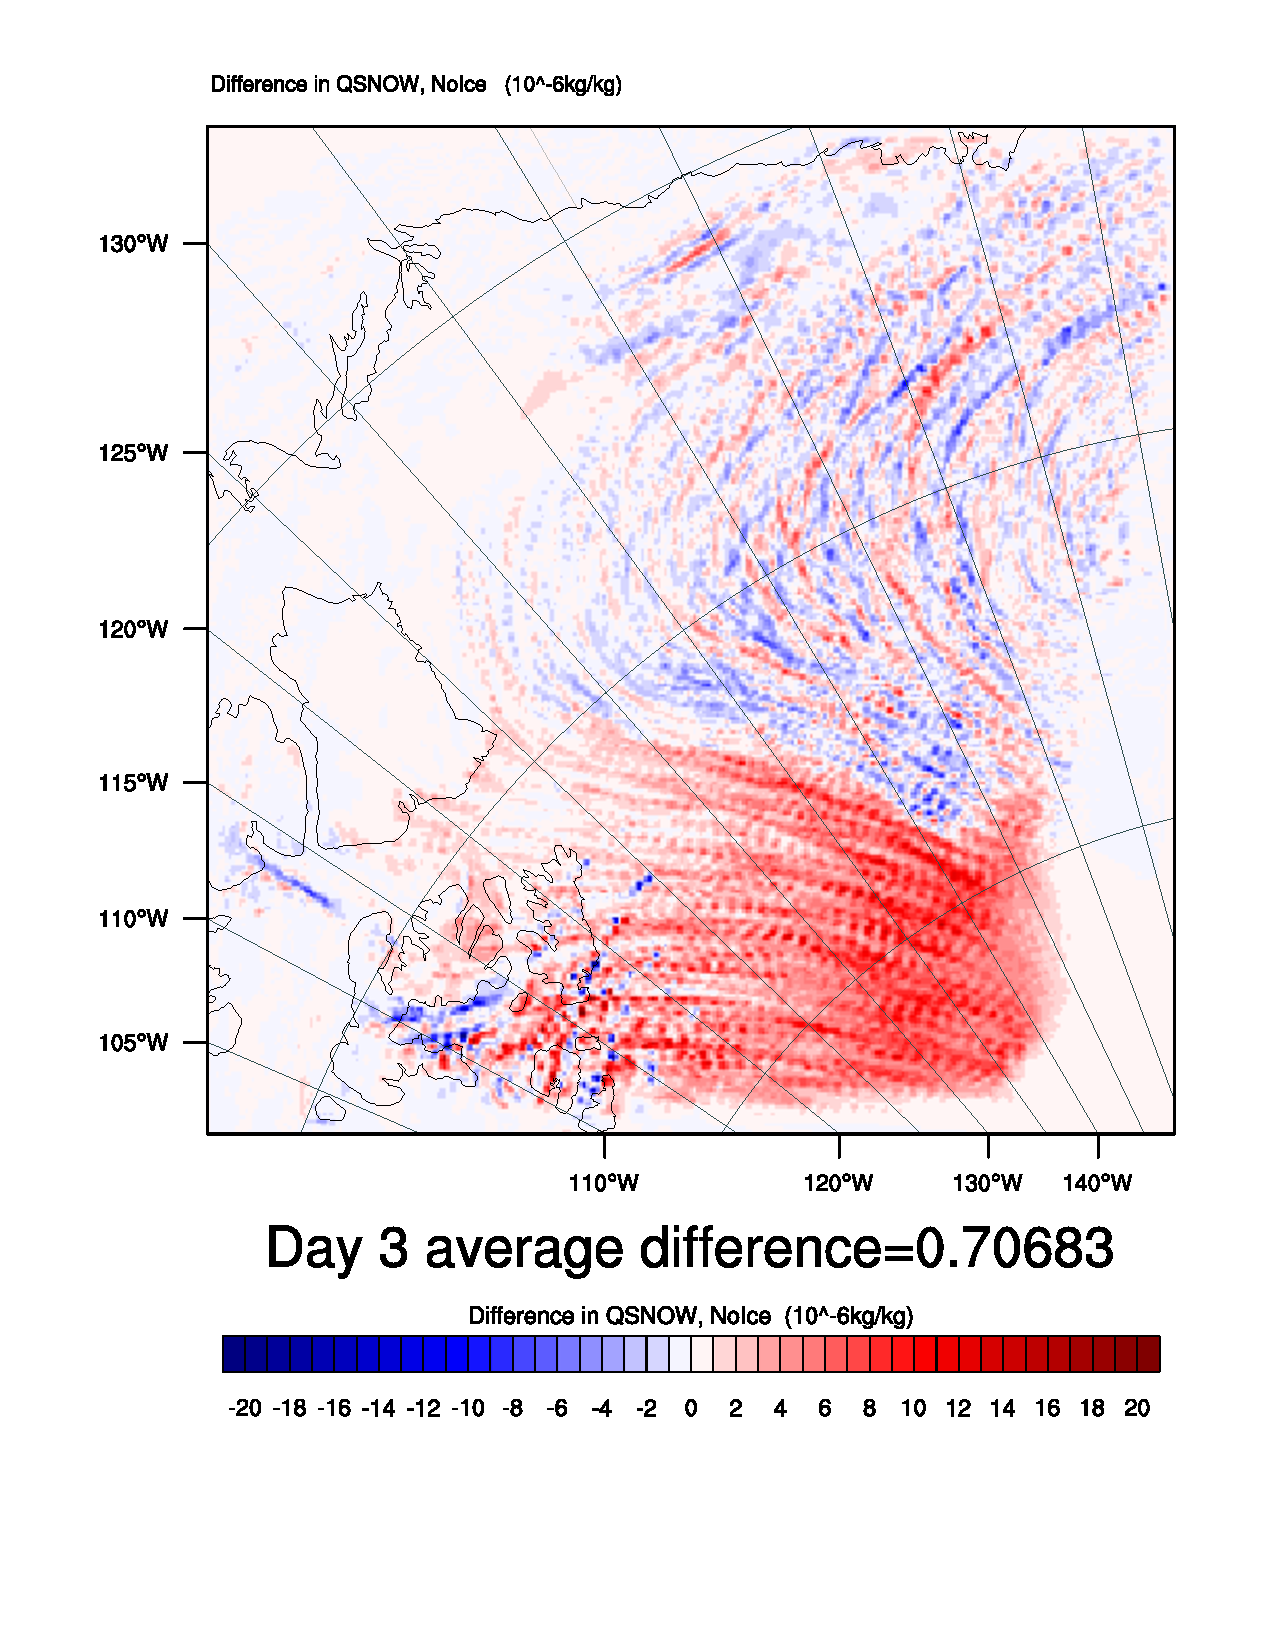
\includegraphics[width=\textwidth]{results/noice/diff_NoIce_qsnow_Day3.pdf}
		\caption{Day 3}
	\end{subfigure}

	\begin{subfigure}{0.32\textwidth}
		\centering
		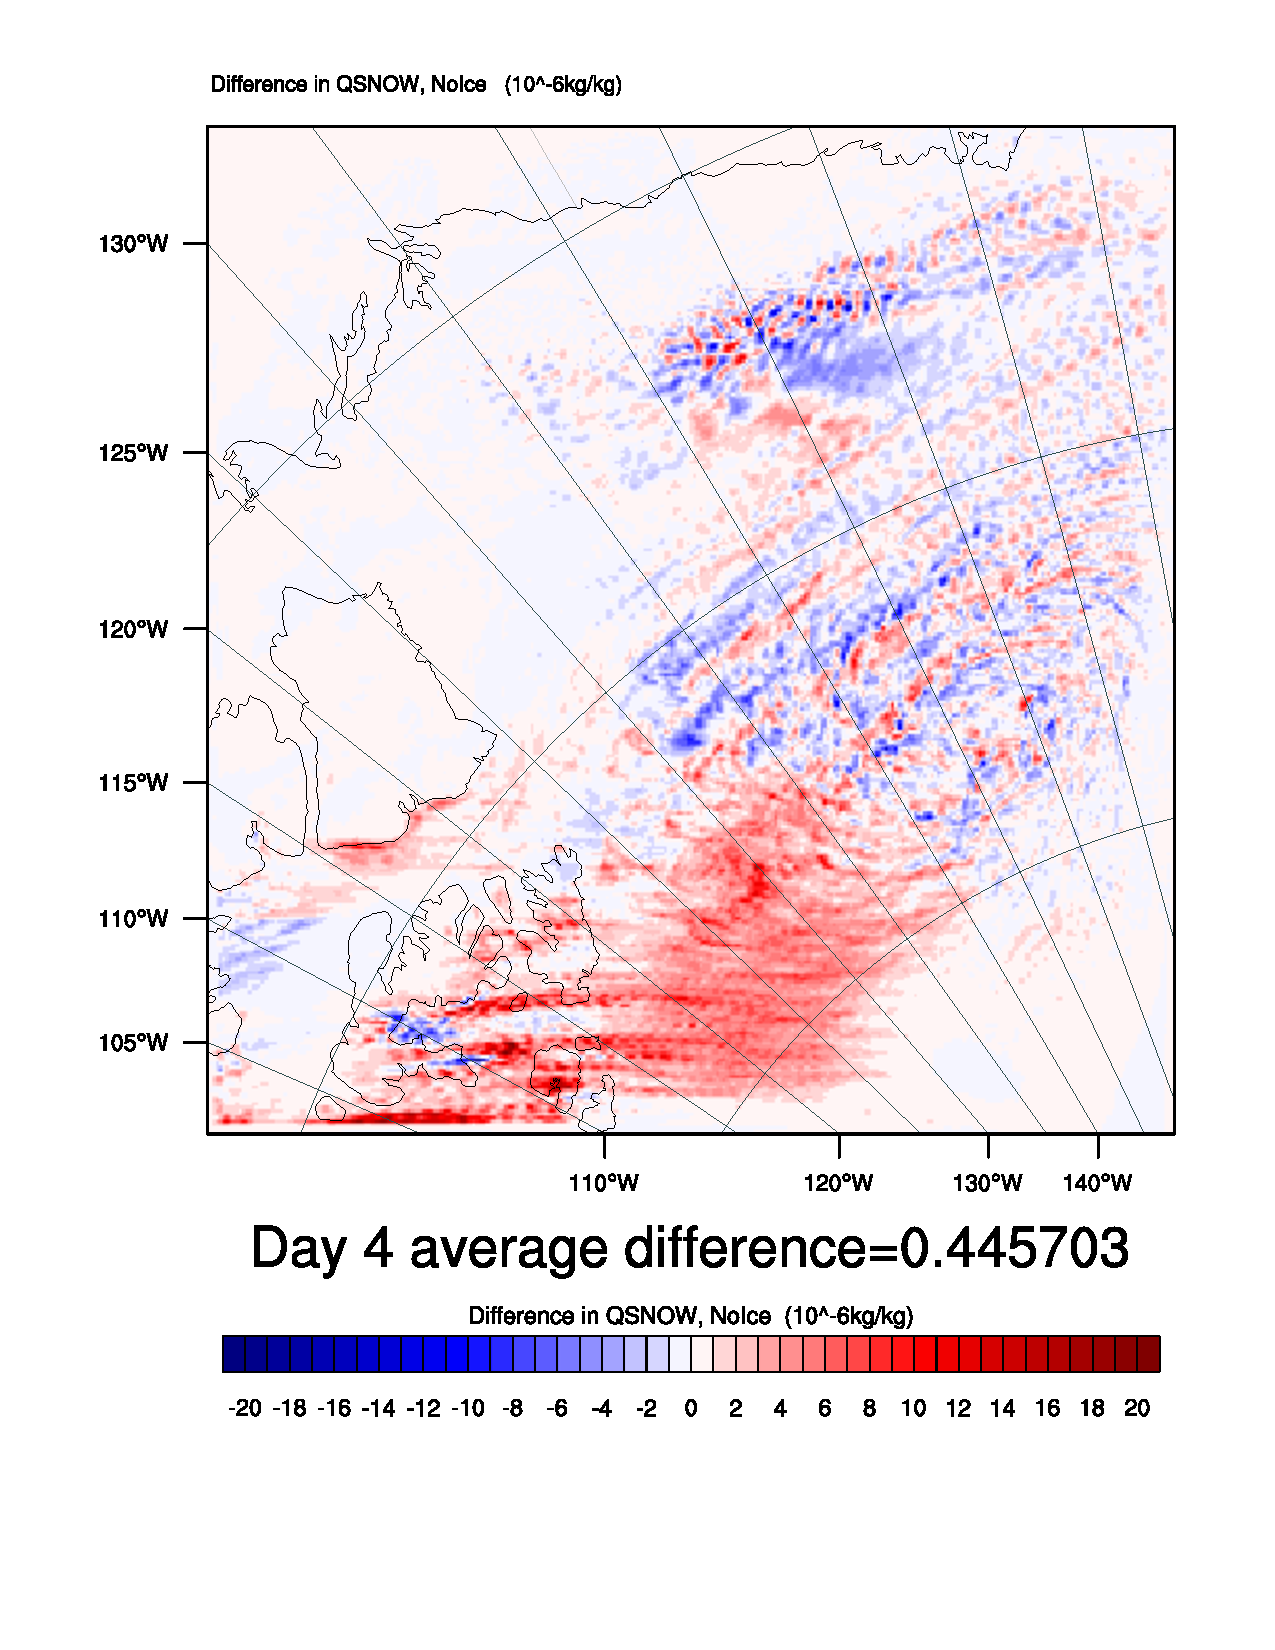
\includegraphics[width=\textwidth]{results/noice/diff_NoIce_qsnow_Day4.pdf}
		\caption{Day 4}
	\end{subfigure}
	\begin{subfigure}{0.32\textwidth}
		\centering
		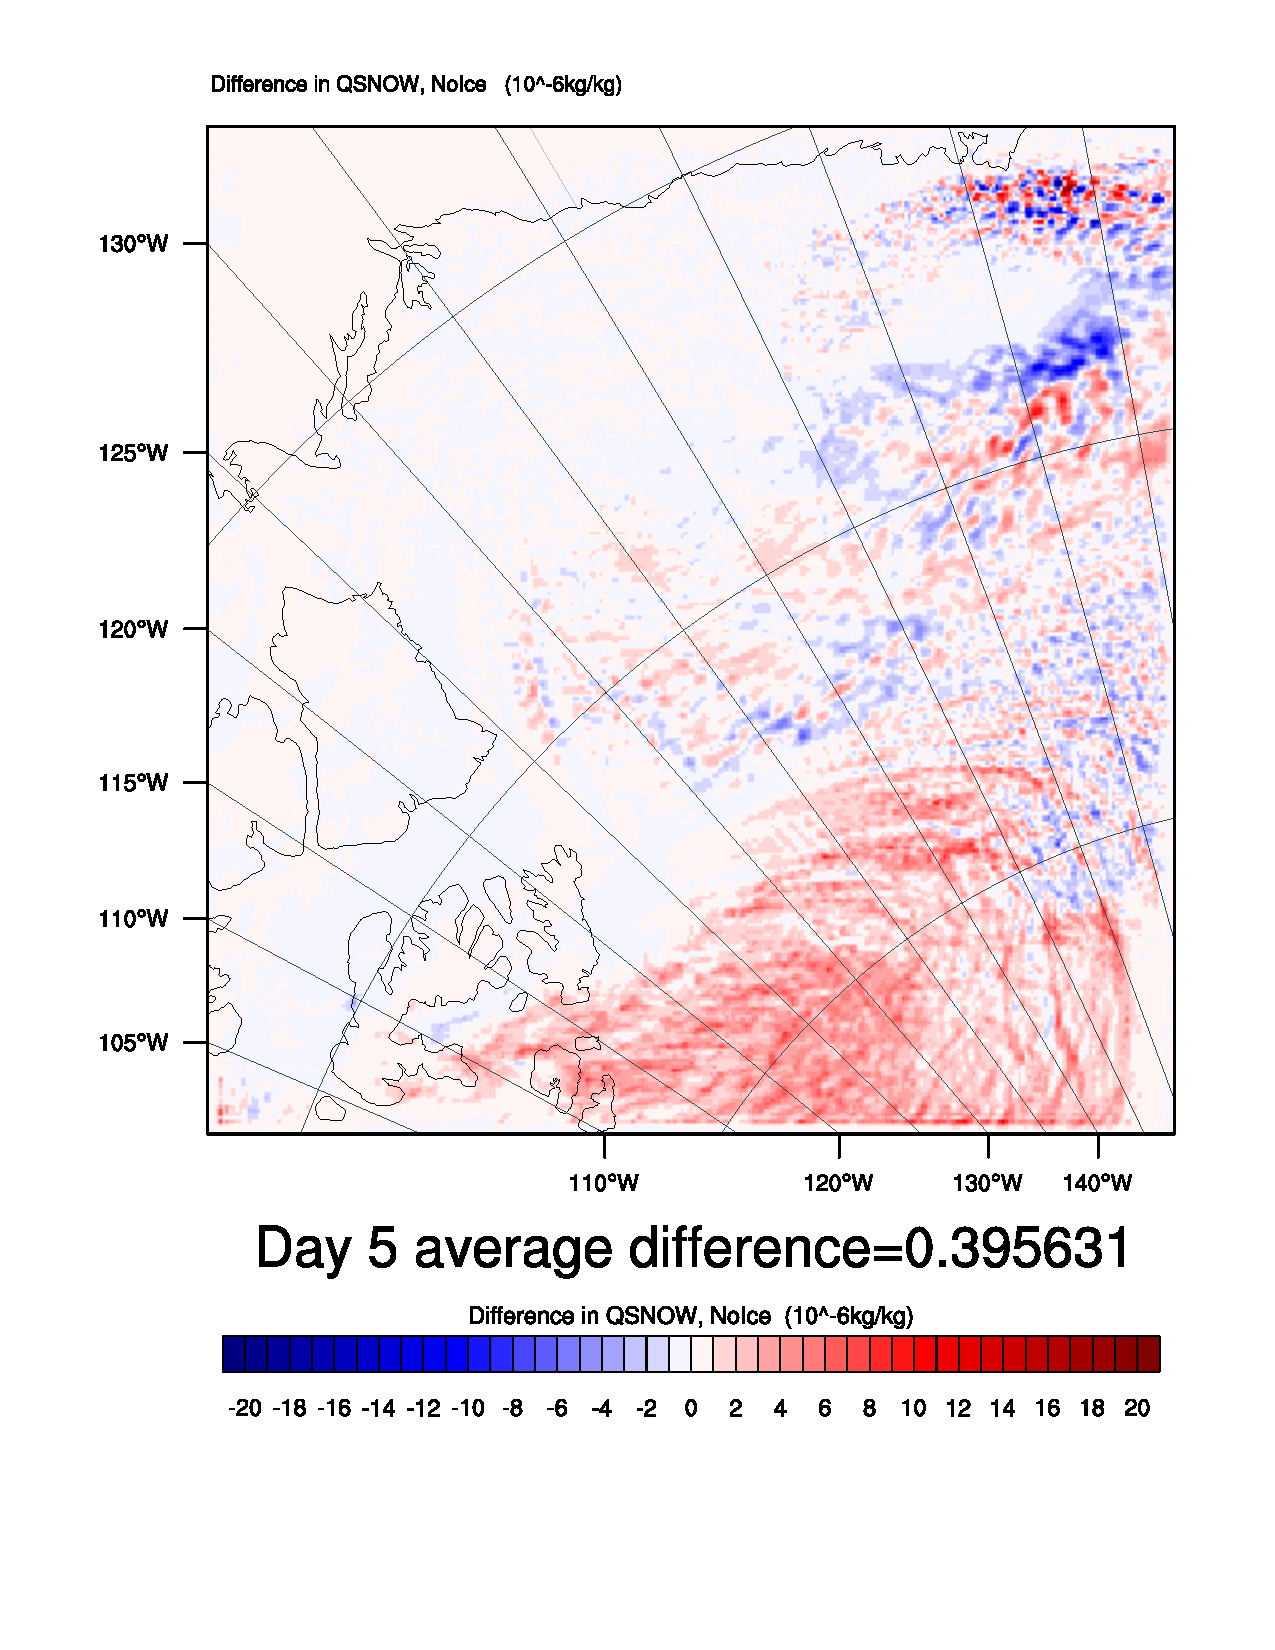
\includegraphics[width=\textwidth]{results/noice/diff_NoIce_qsnow_Day5.pdf}
		\caption{Day 5}
		\label{subfig:snowstory_Day5}
	\end{subfigure}
\caption{Difference in time and height averaged mixing ratio of snow to air, for days 1 to 5. NoIce-Control.}
\label{fig:snowstory}
\end{figure}

Figure~\ref{subfig:snowstory_Day1} shows the difference in mixing ratio of snow to air averaged for day 1 over the 11 lowermost layers. The slight increase in mixing ratio of snow is in the same area as the red patch in figure~\ref{subfig:CDNCr2Day5} that was claimed to be forming clouds. Figure~\ref{subfig:snowstory_Day2} shows that in day 2 the clouds have indeed formed and as time passes more clouds form and produce snow through to day 5, see figure~\ref{subfig:snowstory_Day5} where the positive difference in snow is less pronounced, but still present.

The clouds on the 5th day of the run with no ice are now significantly thinner than the clouds in the 5th day of the control run, due to the aforementioned reduction in CDNC. This allows for more of the upwelling LW at TOA to come directly from the surface (figure~\ref{subfig:lwup_r2Day5}), which holds a higher temperature than the atmosphere above (see cross section in figure~\ref{subfig:cross_LWC_Day5}) and the newly ice free area also has a higher skin temperature, an increase of $\sim$1$\degree$C compared to the control run, when there was sea ice there (see figure~\ref{subfig:skin_r2Day5}). Following Stefan-Boltzmann's law (equation~\ref{eqn:stefanboltzmann}) the surface should then emit more LW than the clouds and sea ice with lower temperatures in the control run did. Figure~\ref{subfig:lwup_r2Day5} shows that the upwelling LW at TOA has indeed increased by $\sim$0.5 to 5 $\text{W/m}^2$ over the area where sea ice has been removed. Overall the average increase in upwelling LW at TOA for the whole area is just shy of 0.5, but the area of particular interest is where the sea ice has been removed, and that shows a more pronounced difference than the rest of the field.

\begin{figure}
\centering
	\begin{subfigure}{0.48\textwidth}
		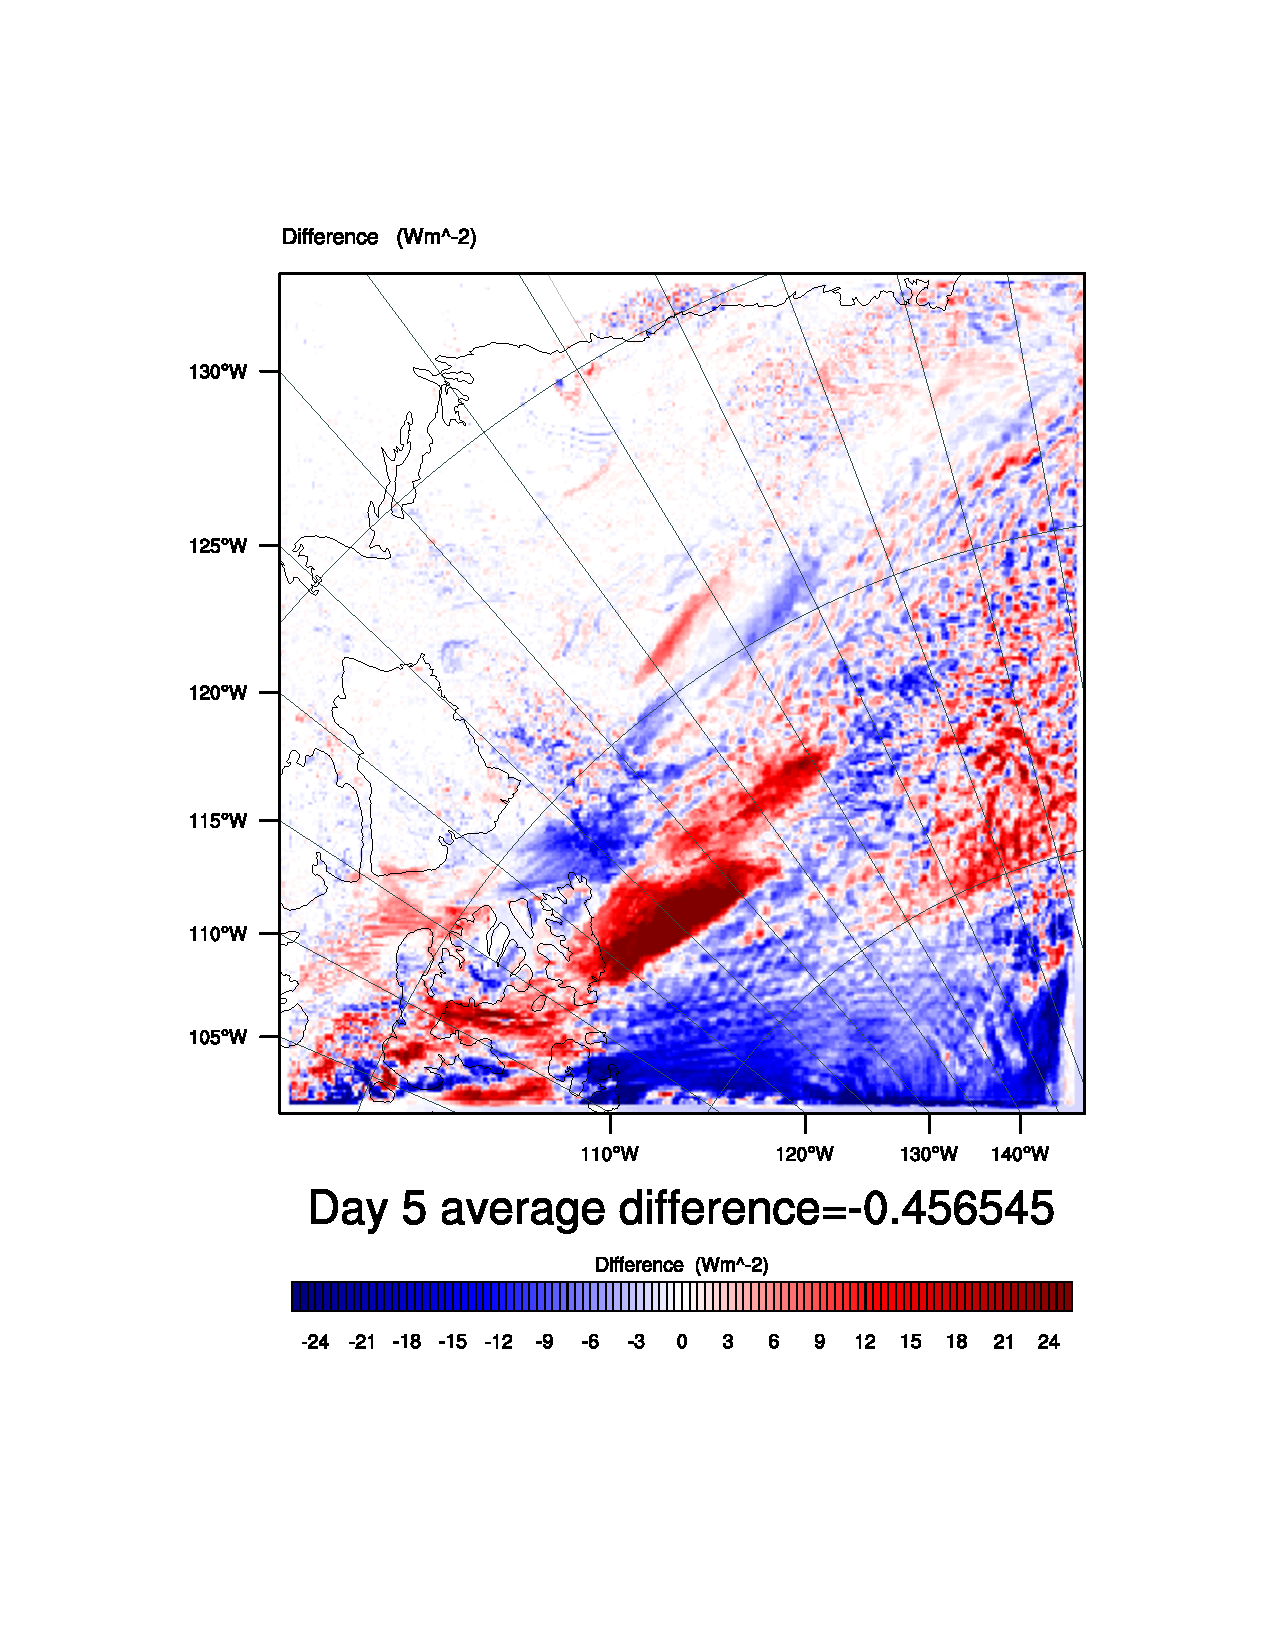
\includegraphics[width=\textwidth]{results/noice/diff_NoIce_SWDOWN_Day5.pdf}
		\caption{SW down at the surface, day 5.}
		\label{subfig:swdown_r2Day5}
	\end{subfigure}
	\quad
	\begin{subfigure}{0.48\textwidth}
		\centering
		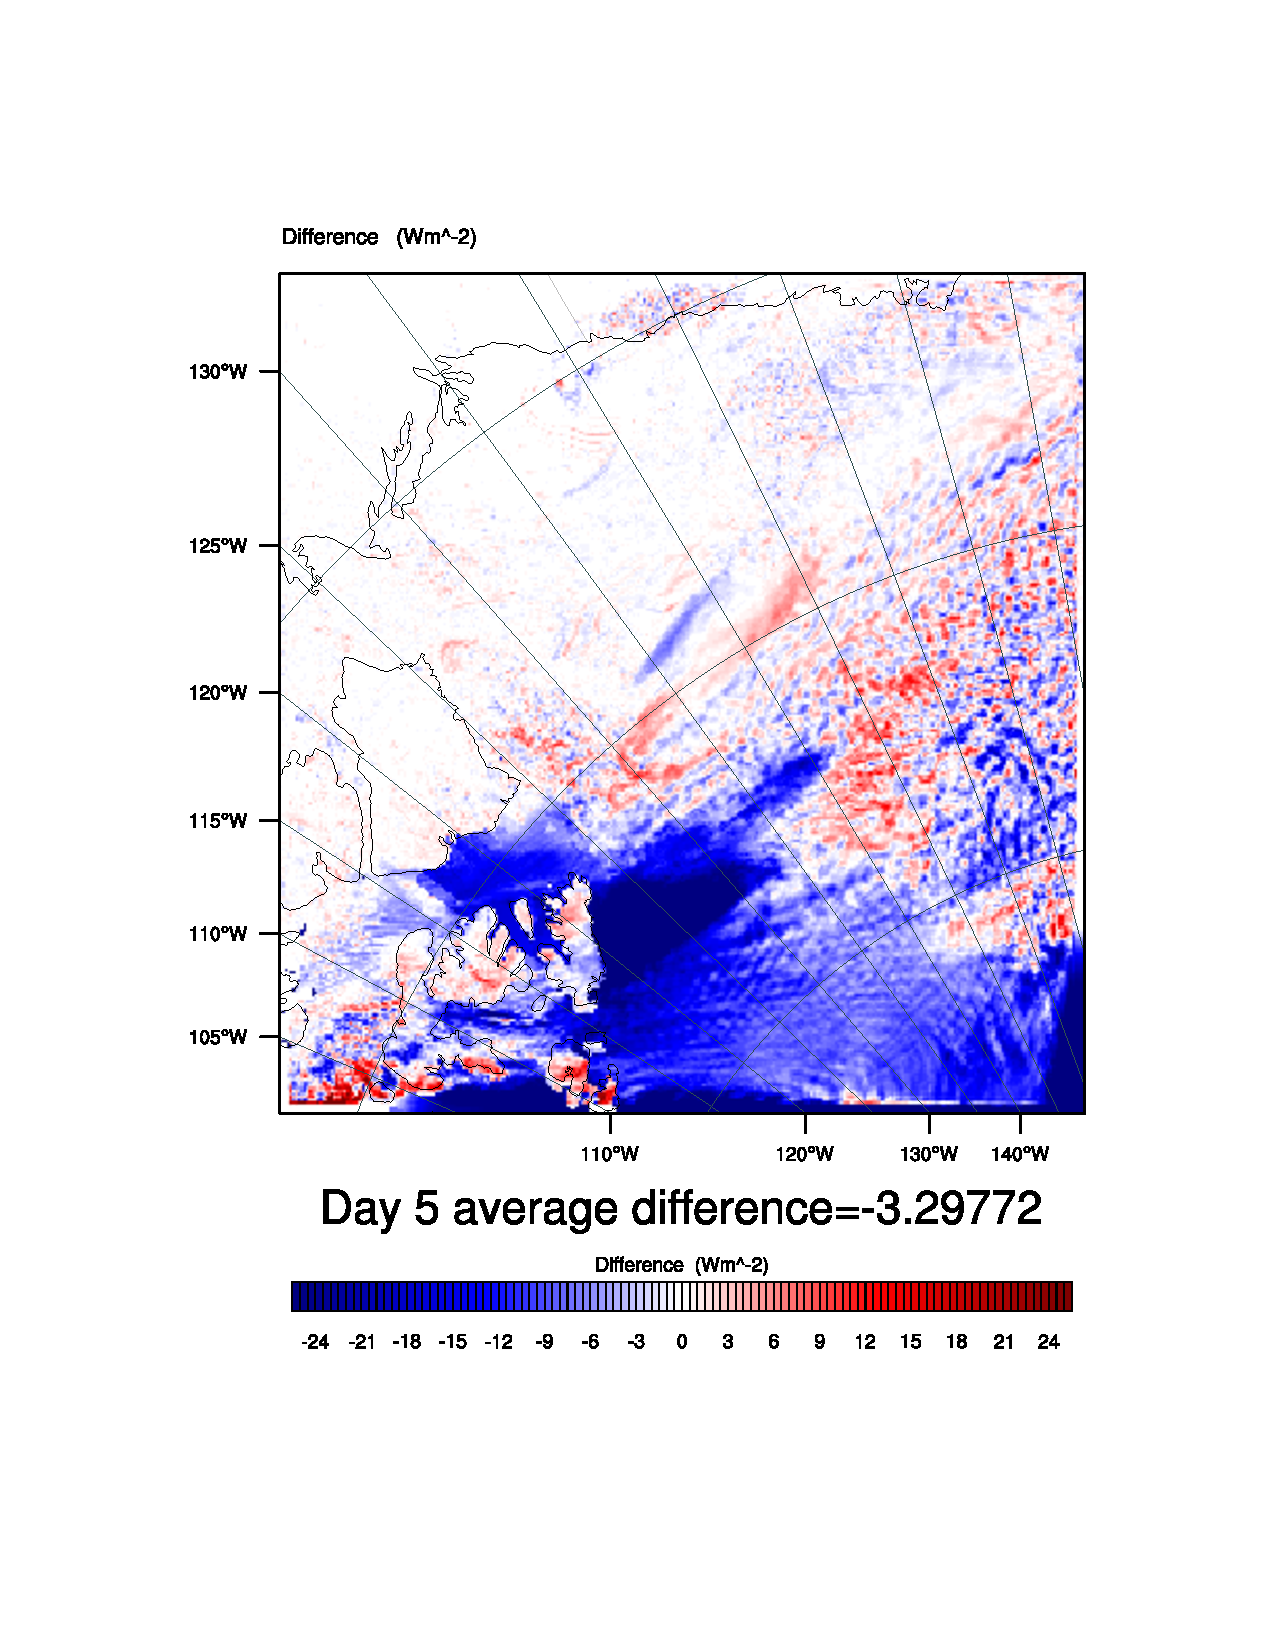
\includegraphics[width=\textwidth]{results/noice/diff_NoIce_SWUPT_Day5.pdf}
		\caption{SW up at TOA, day 5.}
		\label{subfig:swup_r2Day5}
	\end{subfigure}
	
	\begin{subfigure}{0.48\textwidth}
		\centering
		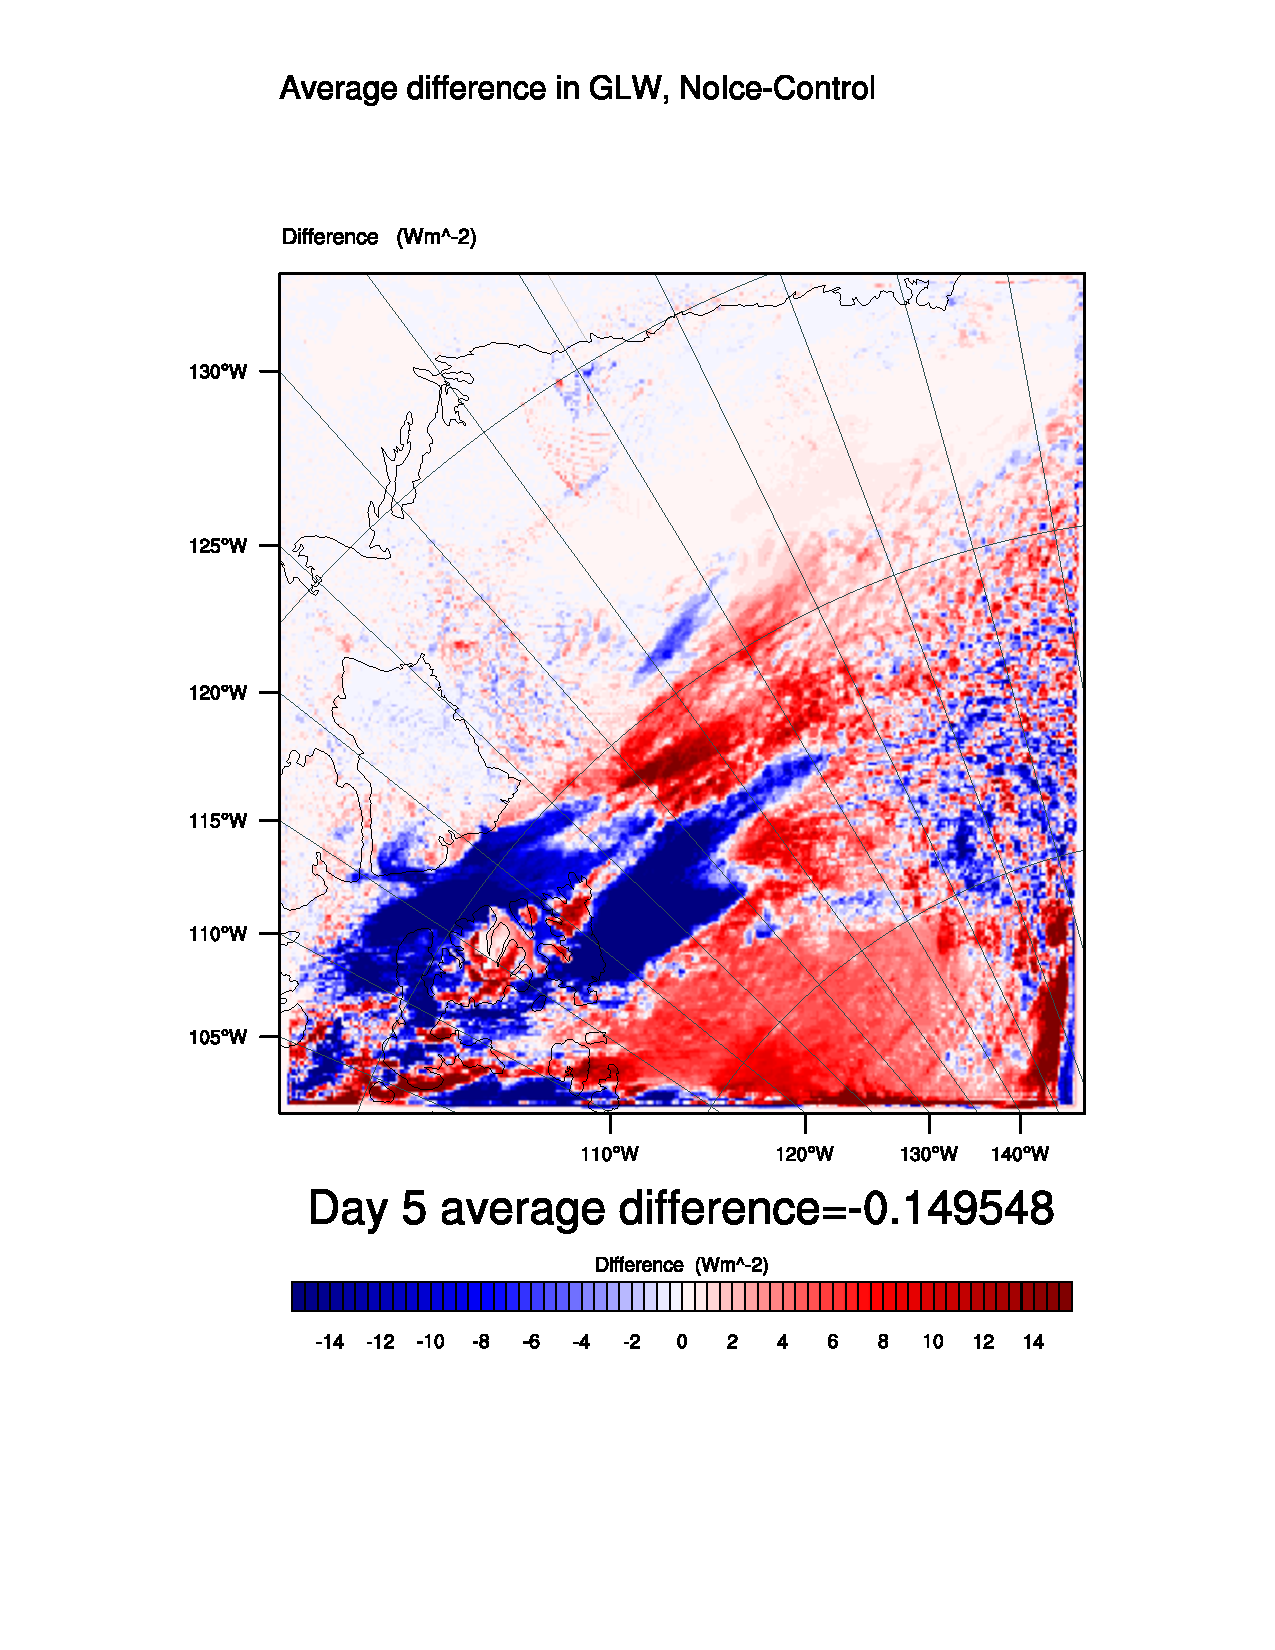
\includegraphics[width=\textwidth]{results/noice/diff_NoIce_GLW_Day5.pdf}
		\caption{LW down at the surface, day 5.}
		\label{subfig:glw_r2Day5}
	\end{subfigure}
	\quad
	\begin{subfigure}{0.48\textwidth}
		\centering
		\includegraphics[width=\textwidth]{results/noice/diff_NoIce_LWUPT_Day5.pdf}
		\caption{LW up at TOA, day 5.}
		\label{subfig:lwup_r2Day5}
	\end{subfigure}
	\caption{Difference in time averaged SW and LW flux down at the surface and up at TOA, for day 5. NoIce-Control.\\Notice the different scales.}
	\label{fig:radiation_r2Day5}
\end{figure}

In figure~\ref{fig:radiation_r2Day5} the difference, for NoIce-Control, in SW down at the surface and up at TOA is illustrated by figures~\ref{subfig:swdown_r2Day5} and~\ref{subfig:swup_r2Day5}. The upwelling SW at TOA (figure~\ref{subfig:swup_r2Day5}) has an average difference of $\sim$-3.3~$\text{W/m}^2$ for the whole field, and from <-25 to around -10~$\text{W/m}^2$ over the now ice free area. Such a decrease in upwelling SW radiation over the whole area that was covered by sea ice in the control run is because of the significant decrease in albedo of the area (not shown), which was discussed under day 1. The most pronounced decrease in upwelling SW at TOA at 77$\degree$N 120-140$\degree$W is of same size and shape as the equally pronounced increase in downwelling SW at the surface of >25~$\text{W/m}^2$ (figure~\ref{subfig:swdown_r2Day5}), in the same place. This can also be recognized as the most significant decrease in CDNC which has lost more than 5 droplets~$\text{cm}^{-3}$ (figure~\ref{subfig:CDNCr2Day5}) compared to the control run. Thus, a cloud that was there in the control run has been significantly thinned or ceased to exist completely, such a decrease in CDNC ($N$ in equation~\ref{eqn:cloudtau1}) decreases the cloud optical depth, $\tau$, and albedo, $A$ (equation~\ref{eqn:cloudalbedo}), and does therefore not protect the surface from downwelling SW by reflecting it back to TOA.

The red patch at 77$\degree$N stretching from 120 to 140$\degree$W, in figure~\ref{subfig:swdown_r2Day5}, indicating the increase in downwelling SW is recognized as a decrease in downwelling LW in the same area in figure~\ref{subfig:glw_r2Day5}. This can also be explained by the decrease in CDNC and the LWP. Looking at the difference in LWP in figure~\ref{subfig:LWPr2Day5}, which shows LWP for NoIce-Control, one sees that the LWP in NoIce is >30~$\text{g/m}^2$ less than in the control run for that exact area. The LW emissivity of the clouds decrease with the LWP (equation~\ref{eqn:epsilon_lw}), provided the LWP is below the limit for saturation in the LW, which is 40-45~$\text{g/m}^2$ according to figure~\ref{fig:epsalb}. The LWP in the control run (figure~\ref{subfig:LWPr1Day5}) for that area was 30 to 60~$\text{g/m}^2$. Thus the LWP in NoIce is below the limit for saturation in LW and the LW emissivity is decreased, explaining the decrease in LW reaching the surface in that particular area.

For quite a large part of the area which is now sea ice free the downwelling LW experiences an increase compared to the control run, see figure~\ref{subfig:glw_r2Day5}. The depletion of clouds by snow, decreasing the LWP, would intuitively also decrease the downwelling LW at the surface if one considers the decrease in emissivity it would lead to, based on equation~\ref{eqn:epsilon_lw}. On the other hand, knowing Stefan-Boltzmann's law (equation~\ref{eqn:stefanboltzmann}) the temperature of the emitting body is of crucial importance. The removal of sea ice has led to an increase in surface heat fluxes and skin temperature, as mentioned in day 1, and shows the same for day 5 in figure~\ref{fig:lhshskin_r2Day5}.

\begin{figure}
\centering
	\begin{subfigure}{0.48\textwidth}
		\includegraphics[width=\textwidth]{results/noice/diff_NoIce_LH_Day5.pdf}
		\caption{Difference in LH.}
		\label{subfig:lh_r2Day5}
	\end{subfigure}
	\quad
		\begin{subfigure}{0.48\textwidth}
		\includegraphics[width=\textwidth]{results/noice/diff_NoIce_HFX_Day5.pdf}
		\caption{Difference in SH.}
		\label{subfig:sh_r2Day5}
	\end{subfigure}
	
	\begin{subfigure}{0.48\textwidth}
		\includegraphics[width=\textwidth]{results/noice/diff_NoIce_skintemp_Day5.pdf}
		\caption{Difference in skin temperature.}
		\label{subfig:skin_r2Day5}
	\end{subfigure}
	\caption{Difference in time averaged LH, SH and skin temperature for day 5. NoIce-Control.}
	\label{fig:lhshskin_r2Day5}
\end{figure}

A higher skin temperature and increased surface heat fluxes causes warmer air to rise, and convection rises the lower cloud base higher up into the atmosphere. The cloud height for a section of the area can be seen in the vertical cross section for LWC on day 5~\ref{fig:cross_LWC_r2Day5} for the run with no ice. Comparing this with the vertical cross section from the control run, figure~\ref{subfig:cross_LWC_Day5}, it is clear that the stratus clouds lie approximately 500~m higher, closer to the mountain in the run without sea ice than they did in the control run.

\begin{figure}
\centering
\includegraphics[width=0.8\textwidth]{results/noice/crossSec_LWC_NoIce_Day5.pdf}
\caption{Time averaged LWC as filled contours, and temperature as dashed contours, in the vertical cross section over the red line in figure~\ref{subfig:cross_line}. Day 5 of NoIce.}
\label{fig:cross_LWC_r2Day5}
\end{figure}

Looking closely at vertical cross sections from NoIce (figure~\ref{fig:cross_LWC_r2Day5}) and Control (figure~\ref{subfig:cross_LWC_Day5}) the clouds in NoIce have a higher temperature at the core (-9$\degree$C), where there is most liquid water, than in Control (-9 to -10$\degree$C). This increase in temperature allow the clouds to emit more LW to the ground surface, following Stefan-Boltzmanns law (equation~\ref{eqn:stefanboltzmann}) than in Control, despite the decrease in LWP that lowers the cloud emissivity (equation~\ref{eqn:epsilon_lw}). On the other hand, in NoIce the clouds do not stretch as close to the mountain as in Control, and at 77$\degree$N and 117$\degree$W (between 100 and 120 on the x-axis) NoIce has no cloud, which fits with the decrease in downwelling LW in that area.

The increase in surface fluxes from the area where sea ice was removed, shown in figure~\ref{fig:lhshskin_r2Day5}, is accompanied by a significant decrease over the ocean outside where the sea ice used to be. Recall that the strong winds in that area made the surface heat fluxes significantly higher over the ocean than over the ice, compared to day 1 (figure~\ref{fig:surface_fluxes_r1}). The wind pattern in NoIce (not shown) is the same as in Control, but since the sea ice is not there, the air being brought over that area is no colder than further out over the ocean and does therefore not experience the same difference in temperature gradient as when the sea ice was there. Thus, removal of sea ice releases more latent and sensible heat, and gives a higher skin temperature ($\sim$0.6 to 2~$\degree$C increase) in that area. With an increase of $\sim$2~$\degree$C the skin temperature (where there used to be sea ice) reaches almost the same skin temperature as the open ocean (figure~\ref{subfig:skin_r1Day5}), thus reducing the temperature gradient between the skin temperature and the overlying air. Therefore there is no marked increase in the surface fluxes off the sea ice edge, and it is shown as a decrease compared to Control, for both LH and SH (figures~\ref{subfig:lh_r2Day5} and~\ref{subfig:sh_r2Day5}).

%-------------------------------------
\clearpage
\section{Increased aerosol number concentration}
%-------------------------------------
The aerosol number concentration was multiplied by 10 to study the effects of pollution in the area. The increased ship traffic in the Arctic leads to higher aerosol loads~\citep{Eckhardt2013}, which could affect the cloud radiative properties and thereby have a warming or cooling effect at the surface. Figure~\ref{fig:aerosols} shows the number concentration for water-friendly aerosols in day 1 of Control and Aero10, where the pattern obviously is almost identical, and overall increased by a factor of 10 (notice the different scales).

\begin{figure}[hb]
\centering
	\begin{subfigure}{0.48\textwidth}
		\centering
		\includegraphics[width=\textwidth]{results/Aero10/Control_QNWFA_Day1.pdf}
		\caption{Control}
		\label{subfig:qnwfa_r1}
	\end{subfigure}
	\begin{subfigure}{0.48\textwidth}
		\centering
		\includegraphics[width=\textwidth]{results/Aero10/Aero10_QNWFA_Day1.pdf}
		\caption{Aero10}
		\label{subfig:qnwfa_r3}
	\end{subfigure}
\caption{Number concentration of water-friendly aerosols in day 1. In Control and Aero10. Notice the different scales.}
\label{fig:aerosols}
\end{figure}


\subsection{Day 1}
With an aerosol number concentration 10 times higher than that in the control run, the average LWP and CDNC for day 1 increase by about 11~$\text{g/m}^2$ and 16~$\text{cm}^{-3}$ respectively, see figure~\ref{fig:lwpcdncre_r3Day1}. The increases in CDNC and LWP are expected with such a high increase in available CCN. The highest increases in LWP and CDNC is where the LWP and CDNC was highest in the control run (figures~\ref{subfig:LWPr1Day1} and~\ref{subfig:cdnc_cont_Day1} respectively), 74-78$\degree$N 145-155$\degree$W and 71$\degree$N 140-150$\degree$W. This increase in time averaged LWP and CDNC indicates that the clouds are denser and longer lived, thereby increasing there reflectance of SW (figure~\ref{subfig:swdown_r3Day1}). This is known as the second indirect effect (recall from Chapter~\ref{chap:theory}).

Remembering the first indirect effect (also described in Chapter~\ref{chap:theory}), one would expect a decrease in droplet size with the increase in numbers. $r_e$ has in fact decreased for the whole field in this run, with and average decrease of 0.5~$\mu\text{m}$, and is shown in figure~\ref{subfig:recloud_r3Day1}

\begin{figure}[hb]
\centering
	\begin{subfigure}{0.48\textwidth}
		\centering
		\includegraphics[width=\textwidth]{results/aero10/Diff_LWP_Day1Aero10.pdf}
		\caption{LWP, Aero10, day 1}
		\label{subfig:LWPr3Day1}
	\end{subfigure}
	\quad
	\begin{subfigure}{0.48\textwidth}
		\centering
		\includegraphics[width=\textwidth]{results/aero10/diff_Aero10_QNCLOUD_Day1.pdf}
		\caption{CDNC, Aero10, day 1}
		\label{subfig:CDNCr3Day1}
	\end{subfigure}
	
	\begin{subfigure}{0.48\textwidth}
		\centering
		\includegraphics[width=\textwidth]{results/aero10/diff_Aero10_RE_CLOUD_Day1.pdf}
		\caption{$r_e$, Aero10, day 1}
		\label{subfig:recloud_r3Day1}
	\end{subfigure}
\caption{Difference in time averaged LWP, and in height and time averaged CDNC and $r_e$, for day 1. Aero10-Control.}
\label{fig:lwpcdncre_r3Day1}
\end{figure}

The first indirect effect describes an increase in the cloud albedo as a consequence of more numerous and smaller droplets, and the upwelling SW at TOA is increased by as much as 7.3~$\text{W/m}^2$ on average for the whole field on day 1 (see figure~\ref{subfig:swup_r3Day1}). As opposed to the run with no ice, the sea ice is unchanged in the run with increased aerosol number concentration (Aero10), so the signal here is clearly an increase in reflected SW. Over the sea ice however the increase in reflected SW is not as large as in the rest of the field, since the sea ice already has a relatively high albedo itself (around 0.6). The increase in the albedo of the clouds has significantly reduced the downwelling SW at the surface (figure~\ref{subfig:swdown_r3Day1}) compared to the control run. The change is $\sim$9.3~$\text{W/m}^2$ decrease on average for the study area, which represents a cooling. On the other hand the average LW radiation at the surface is higher (figure~\ref{subfig:glw_r3Day1}) due to the aforementioned increase in LWP and thereby increased emittance by the clouds, as follows from equation~\ref{eqn:epsilon_lw}. The increase in LW reaching the surface is $\sim$2.3~$\text{W/m}^2$. The most pronounced increase in LW down at the surface is in areas where the LWP in the control run (figure~\ref{subfig:LWPr1Day1}) was lower and therefore not as close to saturation with respect to cloud LW emissivity. Two of these areas are 79$\degree$N, 130-140$\degree$W and 82$\degree$N, 125-145$\degree$W. The decrease in upward LW at TOA (figure~\ref{subfig:lwup_r3Day1}) is due to lower emittance of LW from the clouds than from the surface, since they have lower temperatures than the surface. The vertical temperature distribution over the red line in figure~\ref{subfig:cross_line} can be seen as dashed contours in figure~\ref{fig:cross_LWC_r3Day1}, which also shows the LWC as filled contours. The scales are different, but comparing with figure~\ref{subfig:cross_LWC_day1}, showing LWC in the same section from Control, one can see that the LWC has increased in the clouds seen in the section. The vertical distribution of the clouds is the same for both runs, and the clouds formed by orographic lifting over the mountain have higher LWC than in the control run, since more CCN are activated and allowed to grow into cloud droplets. Thus, the clouds are responsible for more of the LW reaching TOA than in the control run.

\begin{figure}
\centering
	\begin{subfigure}{0.48\textwidth}
		\includegraphics[width=\textwidth]{results/aero10/diff_Aero10_SWDOWN_Day1.pdf}
		\caption{SW down at the surface, day 1.}
		\label{subfig:swdown_r3Day1}
	\end{subfigure}
	\quad
	\begin{subfigure}{0.48\textwidth}
		\centering
		\includegraphics[width=\textwidth]{results/aero10/diff_Aero10_SWUPT_Day1.pdf}
		\caption{SW up at TOA, day 1.}
		\label{subfig:swup_r3Day1}
	\end{subfigure}
	
	\begin{subfigure}{0.48\textwidth}
		\centering
		\includegraphics[width=\textwidth]{results/aero10/diff_Aero10_GLW_Day1.pdf}
		\caption{LW down at the surface, day 1.}
		\label{subfig:glw_r3Day1}
	\end{subfigure}
	\quad
	\begin{subfigure}{0.48\textwidth}
		\centering
		\includegraphics[width=\textwidth]{results/aero10/diff_Aero10_LWUPT_Day1.pdf}
		\caption{LW up at TOA, day 1.}
		\label{subfig:lwup_r3Day1}
	\end{subfigure}
	\caption{Difference in time averaged SW and LW flux down at the surface and up at TOA, for day 1. Aero10-Control.\\Notice the different scales.}
	\label{fig:radiation_r3Day1}
\end{figure}

\begin{figure}
	\centering
	\includegraphics[width=0.8\textwidth]{results/aero10/Sec_LWC_Aero10_Day1.pdf}
	\caption{Time averaged LWC as filled contours, and temperature as dashed contours, in the vertical cross section over the red line in figure~\ref{subfig:cross_line}. Day 1 of Aero10.}
	\label{fig:cross_LWC_r3Day1}
\end{figure}

The LW cloud emissivity is sensitive to an increase in water amount for LWP less than $\sim$40-45~$\text{g/m}^2$. Day 1 in the control run had LWP around 50-150~$\text{g/m}^2$ at 72-79$\degree$N 115-125$\degree$W.
This is also seen in that there is no significant change in LW downward at the surface in that area, see figure~\ref{subfig:glw_r3Day1}. This area with lack of change in LW down is approximately the same area as where there is a negative change in LH and SH upward from the surface over the sea ice, and where the skin temperature has decreased ($\sim$-0.2$\degree$), see figure~\ref{fig:lhshskin_r3Day1}. Since there has been no change in LW at that location there is no warming or cooling effects from the LW, but the change can be explained by the changes in SW radiation. The downward SW at the surface has been significantly decreased (-9.2~$\text{W/m}^2$) as a consequence of the increase in aerosol number concentration, see figure~\ref{subfig:swdown_r3Day1}.

The albedo of the sea ice in Aero10 is around 0.6 (not shown) which means that a fraction of the incident SW radiation is absorbed. Since the amount of incident SW radiation at the surface has been reduced by the cloud cover, the absorbed radiation is less than for a higher incident amount. The ice therefore has a lower temperature (figure~\ref{subfig:skin_r3Day1}) decreasing the temperature gradient between the surface and the overlying air, thus decreasing the upward surface heat fluxes.

The skin temperature, figure~\ref{subfig:skin_r3Day1}, shows that these is an increase over the sea ice, where the surface heat fluxes increase (79$\degree$N 130-140$\degree$W and 82$\degree$N 115-145$\degree$W). These areas coincide with the previously mentioned increase in LW down at the surface (figure~\ref{subfig:glw_r3Day1}), where the clouds in the control run were not saturated with respect to LW (figure~\ref{subfig:LWPr1Day1}). An increase in LW down at the surface ahs a warming effect.

Parts of Canada, islands at 73$\degree$N 115-125$\degree$W and 75-77$\degree$N 105-120$\degree$W, and 68$\degree$N 128-133$\degree$W, and the part of the domain that is in Alaska (70$\degree$N 140-158$\degree$W) experience a decrease in skin temperature, >0.5$\degree$C, compared to the control run (figure~\ref{subfig:skin_r3Day1}), but the ocean does not. These areas are also where the reduction in downward SW at the surface is most significant (figure~\ref{subfig:swdown_r3Day1}), and overpower the the increase in LW down at the surface (figure~\ref{subfig:glw_r3Day1}). It was shown in Chapter~\ref{chap:theory}, that when a cloud is saturated with respect to LW (as a function of LWP) the albedo of the clouds become increasingly important, figure~\ref{fig:epsalb}. Since land has lower heat capacity than the ocean, it responds faster to changes in the downward radiation at the surface. In this study there would be no effect on the sea surface temperatures (SSTs) anyway, because they are constant and the same for all the four runs (Control, NoIce, Aero10, Aero10NoIce). The increase in temperature seen from the removal of sea ice earlier in the chapter (figures~\ref{subfig:skin_r2Day1} and~\ref{subfig:skin_r2Day5}) were simply an adjustment to the SSTs downloaded from ECMWF.

\begin{figure}
\centering
	\begin{subfigure}{0.48\textwidth}
		\includegraphics[width=\textwidth]{results/aero10/diff_Aero10_LH_Day1.pdf}
		\caption{Difference in LH.}
		\label{subfig:lh_r3Day1}
	\end{subfigure}
	\quad
	\begin{subfigure}{0.48\textwidth}
		\includegraphics[width=\textwidth]{results/aero10/diff_Aero10_HFX_Day1.pdf}
		\caption{Difference in SH.}
		\label{subfig:sh_r3Day1}
	\end{subfigure}

	\begin{subfigure}{0.48\textwidth}
		\includegraphics[width=\textwidth]{results/aero10/diff_Aero10_TSK_Day1.pdf}
		\caption{Difference in skin temperature.}
		\label{subfig:skin_r3Day1}
	\end{subfigure}
	\caption{Difference in time averaged LH, SH and skin temperature for day 1. Aero10-Control.}
	\label{fig:lhshskin_r3Day1}
\end{figure}

%-----------------
\clearpage
\subsection{Day 5}
%-----------------
The differences in LWP and CDNC and $r_e$ for day 5 (Aero10-Control) are shown in figure~\ref{fig:lwpcdncre_r3Day5}. As for day 1, the LWP shows an average increase for the whole study area. The increase in LWP on day 5 in Aero10 compared to Control is $\sim$20~$\text{g/m}^2$ and is especially high where the LWP was also high in the control run (see figure~\ref{subfig:LWPr1Day5}). The increase in CDNC has the same pattern as the increase in LWP, which is expected based on equation~\ref{eqn:LWC}. The average increase in CDNC for the study area is $\sim$22~$\text{cm}^{-3}$. Similarly to day 1, evidence of the first indirect effect is suspected since $r_e$ has an average decrease of $\sim$0.6~$\mu\text{m}$, which means that still for day 5 there are more numerous and smaller droplets. Also for $r_e$ the pattern is the same as for LWP, but with opposite sign.
\begin{figure}[hb]
\centering
	\begin{subfigure}{0.48\textwidth}
		\centering
		\includegraphics[width=\textwidth]{results/aero10/Diff_LWP_Day5Aero10.pdf}
		\caption{LWP, Aero10, day 5}
		\label{subfig:LWPr3Day5}
	\end{subfigure}
	\begin{subfigure}{0.48\textwidth}
		\centering
		\includegraphics[width=\textwidth]{results/aero10/diff_Aero10_QNCLOUD_Day5.pdf}
		\caption{CDNC, Aero10, day 5}
		\label{subfig:CDNCr3Day5}
	\end{subfigure}
	\begin{subfigure}{0.48\textwidth}
		\centering
		\includegraphics[width=\textwidth]{results/aero10/diff_Aero10_RE_CLOUD_Day5.pdf}
		\caption{$r_e$, Aero10, day 5}
		\label{subfig:recloud_r3Day5}
	\end{subfigure}
	\caption{Difference in time averaged LWP, and in height and time averaged CDNC and $r_e$, for day 5. Aero10-Control.}
	\label{fig:lwpcdncre_r3Day5}
\end{figure}

Which means that for day 5 the first indirect effect is expected -- a higher cloud albedo as a consequence of more numerous and smaller droplets, and according to figure~\ref{subfig:swdown_r3Day5} the cloud albedo has indeed increased. On average for the whole study area the upward SW at TOA has increased by $\sim$7~$\text{W/m}^2$. Also here the increase in reflected SW is less over the sea ice. As expected, the SW down at the surface is then decreased for the whole field, with an average decrease of 8.6~$\text{W/m}^2$.

Day 5 in the control run had LWP around 60-100~$\text{g/m}^2$ in the middle lower area of figure~\ref{subfig:LWPr1Day5} (72-85$\degree$N 110-140$\degree$W) and up to almost 300~$\text{g/m}^2$ at 75-72$\degree$N 130-160$\degree$W. Recall that this indicated saturation with respect to LW, which is also seen in that there is no significant change in LW downward at the surface in those areas, see figures~\ref{subfig:glw_r3Day5}.

\begin{figure}
\centering
	\begin{subfigure}{0.48\textwidth}
		\includegraphics[width=\textwidth]{results/aero10/diff_Aero10_SWDOWN_Day5.pdf}
		\caption{The average difference in SW flux down at the surface, day 5.}
		\label{subfig:swdown_r3Day5}
	\end{subfigure}
	\quad
	\begin{subfigure}{0.48\textwidth}
		\centering
		\includegraphics[width=\textwidth]{results/aero10/diff_Aero10_SWUPT_Day5.pdf}
		\caption{The average difference in SW flux up at TOA, day 5.}
		\label{subfig:swup_r3Day5}
	\end{subfigure}
	
	\begin{subfigure}{0.48\textwidth}
		\centering
		\includegraphics[width=\textwidth]{results/aero10/diff_Aero10_GLW_Day5.pdf}
		\caption{The average difference in LW flux down at the surface, day 5.}
		\label{subfig:glw_r3Day5}
	\end{subfigure}
	\quad
	\begin{subfigure}{0.48\textwidth}
		\centering
		\includegraphics[width=\textwidth]{results/aero10/diff_Aero10_LWUPT_Day5.pdf}
		\caption{The average difference in LW flux up at TOA, day 5.}
		\label{subfig:lwup_r3Day5}
	\end{subfigure}
	\caption{Difference in time averaged SW and LW flux down at the surface and up at TOA, for day 5. Aero10-Control.\\Notice the different scales.}
	\label{fig:radiation_r3Day5}
\end{figure}

The area with lack of change in LW down (72-85$\degree$N 110-140$\degree$W) is approximately the same area as where there is a negative change in LH and SH upward from the surface over the sea ice, and where the skin temperature has decreased, see figure~\ref{fig:lhshskin_r3Day5}. Also for day 5 this change can be explained by the changes in SW radiation. The downward SW at the surface has been significantly decreased (-8.6~$\text{W/m}^2$) as a consequence of the increase in aerosol number concentration, see figure~\ref{subfig:swdown_r3Day5}.

\begin{figure}
\centering
	\begin{subfigure}{0.48\textwidth}
		\includegraphics[width=\textwidth]{results/aero10/diff_Aero10_LH_Day5.pdf}
		\caption{Difference in LH.}
		\label{subfig:lh_r3Day5}
	\end{subfigure}
	\quad
	\begin{subfigure}{0.48\textwidth}
		\includegraphics[width=\textwidth]{results/aero10/diff_Aero10_HFX_Day5.pdf}
		\caption{Difference in SH.}
		\label{subfig:sh_r3Day5}
	\end{subfigure}

	\begin{subfigure}{0.48\textwidth}
		\includegraphics[width=\textwidth]{results/aero10/diff_Aero10_TSK_Day5.pdf}
		\caption{Difference in skin temperature.}
		\label{subfig:skin_r3Day5}
	\end{subfigure}
	\caption{Difference in time averaged LH, SH and skin temperature for day 5. Aero10-Control.}
	\label{fig:lhshskin_r3Day5}
\end{figure}

Following the same reasoning as for day 1: Because of the first indirect effect, the cloud albedo has increased, and there is less SW down at the surface for the sea ice to absorb. The ice therefore has a lower temperature (figure~\ref{subfig:skin_r3Day5}) decreasing the temperature gradient between the surface and the overlying air, thus decreasing the upward surface heat fluxes.

The skin temperature, figure~\ref{subfig:skin_r3Day5}, for the domain shows a decrease ($\sim$0.5$\degree$C) in the same area as where there is less sensible and latent heat release over the sea ice, but it also shows a decrease over land. The Canadian islands at 73$\degree$N 115-125$\degree$W and 75-77$\degree$N 105-120$\degree$W, and Alaska  at 70$\degree$N 140-158$\degree$W, experience a decrease in skin temperature compared to the control run, but the ocean does not. Again this is because the land has lower heat capacity than the ocean (and that the SSTs are constant).

For the area north of 75$\degree$N where the clouds were not saturated with respect to LW, the pattern of increase in latent and sensible heat (figures~\ref{subfig:lh_r3Day5} and~\ref{subfig:sh_r3Day5}) can be recognized as the areas of increase in LW down at the surface (figure~\ref{subfig:glw_r3Day5}).

In this case, with reduced SW down at the surface and lower skin temperatures, the increase in aerosol number concentration has a cooling effect at the surface.

%------------
\clearpage
\section{Removed sea ice \underline{and}~increased aerosol}
%------------
The effects on radiative cloud properties and the surface by removal of sea ice and increased aerosol number concentration is studied combined. This is to get an idea of the effects of increased pollution from sea traffic as a consequence of more ice free ocean, in combination with more available heat and moisture from the ocean.% @cite someone looking at that and what they found? 
~The results in this section are not discussed as detailed as the results presented in the two previous sections for NoIce and Aero10 separately. This is to avoid too much repetition of the mechanisms behind the differences.

%-----------------
\subsection{Day 1}
%-----------------
The difference in LWP between the run with both removed sea ice and increased aerosol number concentration (Aero10NoIce) and Control for day 1 (figure~\ref{subfig:LWPr4Day1}) is clearly due to the increase is number of aerosols. The increase in LWP for day 1 in NoIce (figure~\ref{subfig:LWPr2Day1}) was on average $\sim$0.2~$\text{g/m}^2$ for the whole field, whereas for Aero10 it was 11~$\text{g/m}^2$, which is also the average increase for Aero10NoIce. The average increase in CDNC (figure~\ref{subfig:CDNCr4Day1}) for Aero10NoIce is also similar to Aero10 (figure~\ref{subfig:CDNCr3Day1}) where both those runs had an average increase of $\sim$15.9~$\text{cm}^{-3}$. The difference in effective radius is also the same with an average decrease in droplet size of about 0.5~$\mu\text{m}$ (see figure~\ref{subfig:recloud_r4Day1} for Aero10NoIce and~\ref{subfig:recloud_r3Day1} for Aero10). For these specific parameters it is clear that the effect of increasing the aerosol number concentration outweighs that of removing the sea ice.

% Figure with LWP, CDNC and r_e
\begin{figure}
\centering
	\begin{subfigure}{0.48\textwidth}
		\centering
		\includegraphics[width=\textwidth]{results/aero10ni/Diff_LWP_Day1Aero10NoIce.pdf}
		\caption{LWP, Aero10NoIce, day 1.}
		\label{subfig:LWPr4Day1}
	\end{subfigure}
	\quad
	\begin{subfigure}{0.48\textwidth}
		\centering
		\includegraphics[width=\textwidth]{results/aero10ni/diff_Aero10NoIce_QNCLOUD_Day1.pdf}
		\caption{CDNC, Aero10NoIce, day 1.}
		\label{subfig:CDNCr4Day1}
	\end{subfigure}
	
	\begin{subfigure}{0.48\textwidth}
		\centering
		\includegraphics[width=\textwidth]{results/aero10ni/diff_Aero10NoIce_RE_CLOUD_Day1.pdf}
		\caption{$r_e$, Aero10NoIce, day 1.}
		\label{subfig:recloud_r4Day1}
	\end{subfigure}
\caption{Difference in time averaged LWP, and in height and time averaged CDNC and $r_e$, for day 1. Aero10NoIce-Control.}
\label{fig:lwpcdncre_r4Day1}
\end{figure}

When looking at the difference in radiation fluxes down at the surface and up at TOA (figure~\ref{fig:radiation_r4Day1}) one can see that both the removal of sea ice and the increase in aerosol number concentration make a difference. For downward SW at the surface (figure~\ref{subfig:swdown_r4Day1}) the average difference can be interpreted as a sum of the difference in NoIce and Aero10. NoIce and Aero10 had average decreases in SW down of $\sim$2.36~$\text{W/m}^2$ (figure~\ref{subfig:swdown_r2Day1}) and $\sim$9.25~$\text{W/m}^2$ (figure~\ref{subfig:swdown_r3Day1}) respectively. When added together they are almost equal to the average difference in Aero10NoIce, which is a decrease of 11.6~$\text{W/m}^2$. Such a decrease in downwelling SW radiation should have a cooling effect at the surface.

% Figure with SW and LW down at surface and up at TOA
\begin{figure}
\centering
	\begin{subfigure}{0.48\textwidth}
		\includegraphics[width=\textwidth]{results/aero10ni/diff_Aero10NoIce_SWDOWN_Day1.pdf}
		\caption{SW down at surface.}
		\label{subfig:swdown_r4Day1}
	\end{subfigure}
	\quad
	\begin{subfigure}{0.48\textwidth}
		\centering
		\includegraphics[width=\textwidth]{results/aero10ni/diff_Aero10NoIce_SWUPT_Day1.pdf}
		\caption{SW up at TOA.}
		\label{subfig:swup_r4Day1}
	\end{subfigure}
	
	\begin{subfigure}{0.48\textwidth}
		\centering
		\includegraphics[width=\textwidth]{results/aero10ni/diff_Aero10NoIce_GLW_Day1.pdf}
		\caption{LW down at surface.}
		\label{subfig:glw_r4Day1}
	\end{subfigure}
	\quad
	\begin{subfigure}{0.48\textwidth}
		\centering
		\includegraphics[width=\textwidth]{results/aero10ni/diff_Aero10NoIce_LWUPT_Day1.pdf}
		\caption{LW up at TOA.}
		\label{subfig:lwup_r4Day1}
	\end{subfigure}
	\caption{Difference in time averaged SW and LW flux down at the surface and up at TOA, for day 1. Aero10NoIce-Control.\\Notice the different scales.}
	\label{fig:radiation_r4Day1}
\end{figure}

It can be seen from figures~\ref{subfig:lh_r4Day1},~\ref{subfig:sh_r4Day1} and~\ref{subfig:skin_r4Day1} showing LH, SH and skin temperature respectively, that there is a decrease in upward surface fluxes and temperature of the surface at 77-79$\degree$N and 115-125$\degree$W, which was explained by the adjustment to SSTs in the area that had sea ice. As the sea ice is removed the temperatures in that area are set to the SSTs and for the higher temperature over the sea ice, that meant a reduction in temperature, but for most of the area that had sea ice the skin temperature is increased. This is expected since the sea surface normally has a higher temperature than ice. Where the temperature is higher, so is the release of sensible and latent heat, and it is lower where the temperature is lower (see figures~\ref{subfig:lh_r4Day1} and~\ref{subfig:sh_r4Day1}). The decrease in temperature over land has been explained (in the previous section about Aero10) by the increase in aerosol number concentration leading to a significant reduction in downward SW at the surface (figure~\ref{subfig:swdown_r4Day1}). Due to the low heat capacity of land compared to water, the land experiences a cooling and the sea surface does not. (Also the SSTs are constant, and would not be affected by any changes in any of the runs in this thesis.)

% Figure with LH, SH and skintemp
\begin{figure}
\centering
	\begin{subfigure}{0.48\textwidth}
		\includegraphics[width=\textwidth]{results/aero10ni/diff_Aero10NoIce_LH_Day1.pdf}
		\caption{Difference in LH.}
		\label{subfig:lh_r4Day1}
	\end{subfigure}
	\quad
	\begin{subfigure}{0.48\textwidth}
		\includegraphics[width=\textwidth]{results/aero10ni/diff_Aero10NoIce_HFX_Day1.pdf}
		\caption{Difference in SH.}
		\label{subfig:sh_r4Day1}
	\end{subfigure}

	\begin{subfigure}{0.48\textwidth}
		\includegraphics[width=\textwidth]{results/aero10ni/diff_Aero10NoIce_TSK_Day1.pdf}
		\caption{Difference in skin temperature.}
		\label{subfig:skin_r4Day1}
	\end{subfigure}
	\caption{Difference in time averaged LH and SH up at the surface, and skin temperature, for day 1. Aero10NoIce-Control.}
	\label{fig:lhshskin_r4Day1}
\end{figure}

%-----------------
\clearpage
\subsection{Day 5}
%-----------------
On the last day of the run, day 5, the atmosphere has had time to adapt to both the sea ice changes and the changes in aerosol number concentration. The increase in LWP of >25~$\text{g/m}^2$ (south of 75$\degree$N and west of 130$\degree$W in figure~\ref{subfig:LWPr4Day5}) is recognized as the area that had highest LWP in the control run (figure~\ref{subfig:LWPr1Day5}) and experienced an increase in NoIce (figure~\ref{subfig:LWPr2Day5}), but a more significant increase as a consequence of more available CCN in Aero10 (figure~\ref{subfig:LWPr3Day5}). Due to snow, the LWP in NoIce was negative on average (figure~\ref{subfig:LWPr2Day5}), and also here it can be seen that precipitation has significantly reduced the LWP over a part of where there was sea ice (77$\degree$N 115-130$\degree$W). The increase in available moisture and surface temperatures, see figures~\ref{subfig:lh_r4Day5} and~\ref{subfig:skin_r4Day5}, from the removal of sea ice gives increased convection, and production of more precipitating clouds. Thus the average increase in LWP of 16.7~$\text{g/m}^2$ is a combined effect of the increase in CCN increasing the LWP, which is known to be proportional to the CDNC (recall equation~\ref{eqn:LWC}), and the the decrease in LWP, that more convection and precipitation has led to through removal of sea ice.

% Figure with LWP, CDNC and r_e
\begin{figure}[hb]
\centering
	\begin{subfigure}{0.48\textwidth}
		\centering
		\includegraphics[width=\textwidth]{results/aero10ni/Diff_LWP_Day5Aero10NoIce.pdf}
		\caption{LWP, Aero10NoIce, day 5.}
		\label{subfig:LWPr4Day5}
	\end{subfigure}
	\quad
	\begin{subfigure}{0.48\textwidth}
		\centering
		\includegraphics[width=\textwidth]{results/aero10ni/diff_Aero10NoIce_QNCLOUD_Day5.pdf}
		\caption{CDNC, Aero10NoIce, day 5.}
		\label{subfig:CDNCr4Day5}
	\end{subfigure}
	
	\begin{subfigure}{0.48\textwidth}
		\centering
		\includegraphics[width=\textwidth]{results/aero10ni/diff_Aero10NoIce_RE_CLOUD_Day5.pdf}
		\caption{$r_e$, Aero10NoIce, day 5.}
		\label{subfig:recloudr4Day5}
	\end{subfigure}
\caption{Difference in time averaged LWP, and in height and time averaged CDNC and $r_e$, for day 5. Aero10NoIce-Control.}
\label{fig:lwpcdncre_r4Day5}
\end{figure}

The most pronounced decrease in LWP (77$\degree$N 115-130$\degree$W), has here as in NoIce, opened up for a significant increase of $\sim$20~$\text{W/m}^2$ in SW down at the surface at tha location, seen as the only red patch in figure~\ref{subfig:swdown_r4Day5}. Since the ocean albedo is 0.06, and not 0.6 as it was for the sea ice, the SW up at TOA has also changed by $\sim$20~$\text{W/m}^2$, but with opposite sign (figure~\ref{subfig:swup_r4Day5}). This thinning of the clouds has led to changes in LW too, where the LW down at the surface is decreased by $\sim$15~$\text{W/m}^2$ (figure~\ref{subfig:glw_r4Day5}), and the LW up at TOA has increased by up to 5~$\text{W/m}^2$ (figure~\ref{subfig:lwup_r4Day5}). The increase in LW up at TOA is because of the increased surface temperature seen in figure~\ref{subfig:skin_r4Day5} (recall Stefan-Boltzmann's law, equation~\ref{eqn:stefanboltzmann}).

% Figure with SW and LW down at surface and up at TOA
\begin{figure}
\centering
	\begin{subfigure}{0.48\textwidth}
		\includegraphics[width=\textwidth]{results/aero10ni/diff_Aero10NoIce_SWDOWN_Day5.pdf}
		\caption{SW down at the surface.}
		\label{subfig:swdown_r4Day5}
	\end{subfigure}
	\quad
	\begin{subfigure}{0.48\textwidth}
		\centering
		\includegraphics[width=\textwidth]{results/aero10ni/diff_Aero10NoIce_SWUPT_Day5.pdf}
		\caption{SW up at TOA.}
		\label{subfig:swup_r4Day5}
	\end{subfigure}
	
	\begin{subfigure}{0.48\textwidth}
		\centering
		\includegraphics[width=\textwidth]{results/aero10ni/diff_Aero10NoIce_GLW_Day5.pdf}
		\caption{LW down at the surface.}
		\label{subfig:glw_r4Day5}
	\end{subfigure}
	\quad
	\begin{subfigure}{0.48\textwidth}
		\centering
		\includegraphics[width=\textwidth]{results/aero10ni/diff_Aero10NoIce_LWUPT_Day5.pdf}
		\caption{LW up at TOA.}
		\label{subfig:lwup_r4Day5}
	\end{subfigure}
	\caption{The average difference in SW and LW flux down at the surface and up at TOA, for day 5. Aero10NoIce-Control.\\Notice the different scales.}
	\label{fig:radiation_r4Day5}
\end{figure}

The difference in surface heat fluxes is dominated by the removal of sea ice, see figures~\ref{subfig:lh_r4Day5} and~\ref{subfig:sh_r4Day5}. The reason for the patterns seen in those figures is that the removal of sea ice increases the surface temperature (figure~\ref{subfig:skin_r4Day5}), which strengthens the temperature gradient between the surface and the overlying air. Thus the surface fluxes are increased where the sea ice has been removed. Just off the sea ice edge on the other hand there is a strong decrease is surface heat fluxes. This decrease is simply showing (compared to Control in figure~\ref{fig:surface_fluxes_r1}) that there is not a pronounced increase in surface heat fluxes off the sea ice edge, now that the surface temperature is almost the same where there used to be sea ice, and just outside that area, giving a much smaller temperature gradient than in the control run, despite the strong winds. One may also recall the decrease in SH and skin temperature over the Canadian islands and Alaska, from increase in aerosol number concentration (figure~\ref{fig:lhshskin_r3Day5}) which is also noticeable in figures~\ref{subfig:sh_r4Day5} and~\ref{subfig:skin_r4Day5}.

% Figure with LH, SH and skintemp
\begin{figure}
\centering
	\begin{subfigure}{0.48\textwidth}
		\includegraphics[width=\textwidth]{results/aero10ni/diff_Aero10NoIce_LH_Day5.pdf}
		\caption{Difference in LH.}
		\label{subfig:lh_r4Day5}
	\end{subfigure}
	\quad
	\begin{subfigure}{0.48\textwidth}
		\includegraphics[width=\textwidth]{results/aero10ni/diff_Aero10NoIce_HFX_Day5.pdf}
		\caption{Difference in SH.}
		\label{subfig:sh_r4Day5}
	\end{subfigure}

	\begin{subfigure}{0.48\textwidth}
		\includegraphics[width=\textwidth]{results/aero10ni/diff_Aero10NoIce_TSK_Day5.pdf}
		\caption{Difference in skin temperature.}
		\label{subfig:skin_r4Day5}
	\end{subfigure}
	\caption{Average difference in LH and SH up at the surface, and difference in skin temperature, for day 5. Aero10NoIce-Control.}
	\label{fig:lhshskin_r4Day5}
\end{figure}

The increase in surface heat fluxes and skin temperature (figure~\ref{fig:lhshskin_r4Day5}) where the sea ice has been removed causes increased convection. Figure~\ref{fig:cross_LWC_r4Day5} shows LWC and temperature in the vertical cross section over the red line in figure~\ref{subfig:cross_line}. There it is clear that the cloud base has been elevated due to the increased convection, compared to the control run (see figure~\ref{subfig:cross_LWC_Day5}). The loss of liquid water near the mountain, is covered by the area of most pronounced decrease in LWP, indicated by the dark blue patch at 77$\degree$N 115-130$\degree$W.

Looking at the cross sections of LWC and temperature from Aero10NoIce and Control (figures~\ref{fig:cross_LWC_r4Day5} and~\ref{subfig:cross_LWC_Day5}) one can also see that the temperature is higher in Aero10NoIce. Where there is most liquid water in Aero10NoIce the temperature is $\sim$-8 to -9$\degree$C, whereas in Control it is $\sim$-9 to -10$\degree$C. This contributes tho an increase in downwelling LW at the surface (figure~\ref{subfig:glw_r4Day5}).

\begin{figure}
	\centering
	\includegraphics[width=0.8\textwidth]{results/aero10ni/Sec_LWC_Aero10NoIce_Day5.pdf}
	\caption{Time averaged LWC as filled contours, and temperature as dashed contours, in the vertical cross section over the red line in figure~\ref{subfig:cross_line}. Day 5 of Aero10NoIce.}
	\label{fig:cross_LWC_r4Day5}
\end{figure}